% ******************************* PhD Thesis Template **************************
% Please have a look at the README.md file for info on how to use the template
% https://github.com/kks32/phd-thesis-template/blob/master/README.md

\documentclass[a4paper,12pt,times,numbered,print,oneside]{Classes/PhDThesisPSnPDF}

% ******************************************************************************
% ******************************* Class Options ********************************
% *********************** See README for more details **************************
% ******************************************************************************

% `a4paper'(The University of Cambridge PhD thesis guidelines recommends a page
% size a4 - default option) or `a5paper': A5 Paper size is also allowed as per
% the Cambridge University Engineering Deparment guidelines for PhD thesis
%
% `11pt' or `12pt'(default): Font Size 10pt is NOT recommended by the University
% guidelines
%
% `oneside' or `twoside'(default): Printing double side (twoside) or single
% side.
%
% `print': Use `print' for print version with appropriate margins and page
% layout. Leaving the options field blank will activate Online version.
%
% `index': For index at the end of the thesis
%
% `draftclassic': For draft mode without loading any images (same as draft in book)
%
% `draft': Special draft mode with line numbers, images, and water mark with
% timestamp and custom text. Position of the text can also be modified.
%
% `abstract': To generate only the title page and abstract page with
% dissertation title and name, to submit to the Student Registry
%
% `chapter`: This option enables only the specified chapter and it's references
%  Useful for review and corrections.
%
% ************************* Custom Page Margins ********************************
%
% `custommargin`: Use `custommargin' in options to activate custom page margins,
% which can be defined in the preamble.tex. Custom margin will override
% print/online margin setup.
%
% *********************** Choosing the Fonts in Class Options ******************
%
% `times' : Times font with math support. (The Cambridge University guidelines
% recommend using times)
%
% `fourier': Utopia Font with Fourier Math font (Font has to be installed)
%            It's a free font.
%
% `customfont': Use `customfont' option in the document class and load the
% package in the preamble.tex
%
% default or leave empty: `Latin Modern' font will be loaded.
%
% ********************** Choosing the Bibliography style ***********************
%
% `authoryear': For author-year citation eg., Krishna (2013)
%
% `numbered': (Default Option) For numbered and sorted citation e.g., [1,5,2]
%
% `custombib': Define your own bibliography style in the `preamble.tex' file.
%              `\RequirePackage[square, sort, numbers, authoryear]{natbib}'.
%              This can be also used to load biblatex instead of natbib
%              (See Preamble)
%
% **************************** Choosing the Page Style *************************
%
% `default (leave empty)': For Page Numbers in Header (Left Even, Right Odd) and
% Chapter Name in Header (Right Even) and Section Name (Left Odd). Blank Footer.
%
% `PageStyleI': Chapter Name next & Page Number on Even Side (Left Even).
% Section Name & Page Number in Header on Odd Side (Right Odd). Footer is empty.
%
% `PageStyleII': Chapter Name on Even Side (Left Even) in Header. Section Number
% and Section Name in Header on Odd Side (Right Odd). Page numbering in footer

% Uncomment to change page style
\pagestyle{PageStyleII}

% ********************************** Preamble **********************************
% Preamble: Contains packages and user-defined commands and settings
% ******************************************************************************
% ****************************** Custom Margin *********************************

% Add `custommargin' in the document class options to use this section
% Set {innerside margin / outerside margin / topmargin / bottom margin}  and
% other page dimensions
\ifsetCustomMargin
  \RequirePackage[left=37mm,right=30mm,top=35mm,bottom=30mm]{geometry}
  \setFancyHdr % To apply fancy header after geometry package is loaded
\fi

% Add spaces between paragraphs
%\setlength{\parskip}{0.5em}
% Ragged bottom avoids extra whitespaces between paragraphs
\raggedbottom
% To remove the excess top spacing for enumeration, list and description
%\usepackage{enumitem}
%\setlist[enumerate,itemize,description]{topsep=0em}

% *****************************************************************************
% ******************* Fonts (like different typewriter fonts etc.)*************

% Add `customfont' in the document class option to use this section

\ifsetCustomFont
  % Set your custom font here and use `customfont' in options. Leave empty to
  % load computer modern font (default LaTeX font).
  %\RequirePackage{helvet}

  % For use with XeLaTeX
  %  \setmainfont[
  %    Path              = ./libertine/opentype/,
  %    Extension         = .otf,
  %    UprightFont = LinLibertine_R,
  %    BoldFont = LinLibertine_RZ, % Linux Libertine O Regular Semibold
  %    ItalicFont = LinLibertine_RI,
  %    BoldItalicFont = LinLibertine_RZI, % Linux Libertine O Regular Semibold Italic
  %  ]
  %  {libertine}
  %  % load font from system font
  %  \newfontfamily\libertinesystemfont{Linux Libertine O}
\fi

% *****************************************************************************
% **************************** Custom Packages ********************************

% ************************* Algorithms and Pseudocode *************************

%\usepackage{algpseudocode}


% ********************Captions and Hyperreferencing / URL **********************

% Captions: This makes captions of figures use a boldfaced small font.
%\RequirePackage[small,bf]{caption}

\RequirePackage[labelsep=space,tableposition=top]{caption}


% *************************** Graphics and figures *****************************

%\usepackage{rotating}
%\usepackage{wrapfig}

% Uncomment the following two lines to force Latex to place the figure.
% Use [H] when including graphics. Note 'H' instead of 'h'
\usepackage{float}
\restylefloat{figure}

% Subcaption package is also available in the sty folder you can use that by
% uncommenting the following line
% This is for people stuck with older versions of texlive
%\usepackage{sty/caption/subcaption}
\usepackage{subcaption}

% ********************************** Tables ************************************
\usepackage{booktabs} % For professional looking tables
\usepackage{multirow}

%\usepackage{multicol}
%\usepackage{longtable}
%\usepackage{tabularx}


% *********************************** SI Units *********************************
% \usepackage{siunitx} % use this package module for SI units


% ******************************* Line Spacing *********************************

% Choose linespacing as appropriate. Default is one-half line spacing as per the
% University guidelines

% \doublespacing
% \onehalfspacing
% \singlespacing


% ************************ Formatting / Footnote *******************************

% Don't break enumeration (etc.) across pages in an ugly manner (default 10000)
%\clubpenalty=500
%\widowpenalty=500

%\usepackage[perpage]{footmisc} %Range of footnote options


% *****************************************************************************
% *************************** Bibliography  and References ********************

%\usepackage{cleveref} %Referencing without need to explicitly state fig /table

% Add `custombib' in the document class option to use this section
\ifuseCustomBib
   \RequirePackage[square, compress, numbers, authoryear]{natbib} % CustomBib

% If you would like to use biblatex for your reference management, as opposed to the default `natbibpackage` pass the option `custombib` in the document class. Comment out the previous line to make sure you don't load the natbib package. Uncomment the following lines and specify the location of references.bib file

%\RequirePackage[backend=biber, style=numeric-comp, citestyle=numeric, sorting=nty, natbib=true]{biblatex}
%\addbibresource{References/references} %Location of references.bib only for biblatex, Do not omit the .bib extension from the filename.

\fi

% changes the default name `Bibliography` -> `References'
\renewcommand{\bibname}{References}


% ******************************************************************************
% ************************* User Defined Commands ******************************
% ******************************************************************************

% *********** To change the name of Table of Contents / LOF and LOT ************

\renewcommand{\contentsname}{Table of Contents}
\renewcommand{\listfigurename}{List of Figures}
\renewcommand{\listtablename}{List of Tables}


% ********************** TOC depth and numbering depth *************************

\setcounter{secnumdepth}{4}
\setcounter{tocdepth}{1}


% ******************************* Nomenclature *********************************

% To change the name of the Nomenclature section, uncomment the following line

\renewcommand{\nomname}{List of Abbreviations}


% ********************************* Appendix ***********************************

% The default value of both \appendixtocname and \appendixpagename is `Appendices'. These names can all be changed via:

%\renewcommand{\appendixtocname}{List of appendices}
%\renewcommand{\appendixname}{Appndx}

% *********************** Configure Draft Mode **********************************

% Uncomment to disable figures in `draft'
%\setkeys{Gin}{draft=true}  % set draft to false to enable figures in `draft'

% These options are active only during the draft mode
% Default text is "Draft"
%\SetDraftText{DRAFT}

% Default Watermark location is top. Location (top/bottom)
%\SetDraftWMPosition{bottom}

% Draft Version - default is v1.0
%\SetDraftVersion{v1.1}

% Draft Text grayscale value (should be between 0-black and 1-white)
% Default value is 0.75
%\SetDraftGrayScale{0.8}


% ******************************** Todo Notes **********************************
%% Uncomment the following lines to have todonotes.

%\ifsetDraft
%	\usepackage[colorinlistoftodos]{todonotes}
%	\newcommand{\mynote}[1]{\todo[author=kks32,size=\small,inline,color=green!40]{#1}}
%\else
%	\newcommand{\mynote}[1]{}
%	\newcommand{\listoftodos}{}
%\fi

% Example todo: \mynote{Hey! I have a note}

% *****************************************************************************
% ******************* Better enumeration my MB ********************************
\usepackage{enumitem}

\usepackage{bm}
\usepackage{bbm}
\usepackage{pdfpages}

\newcommand{\SectionsDir}{}
\newcommand{\FigsDir}{}
\newcommand{\TablesDir}{}

\def\Figure[#1][#2]#3#4{%
  \begin{figure}[#1]%
    \centering%
    \includegraphics[#2]{#3}%
    \vspace{5pt}%
    \caption{#4}%
  \end{figure}
}

\def\Table[#1]#2#3{%
  \begin{table}[#1]%
    \caption{#3}%
    \vspace{5pt}%
    \centering%
    \input{#2}%
  \end{table}%
}

\definecolor{accessblue}{cmyk}{0.95,0.50,0.00,0.12}
\renewcommand{\figurename}{FIGURE}
\renewcommand\tablename{TABLE}
\captionsetup{labelfont={color=accessblue, bf}, font={small, sf}}

% ************************ Thesis Information & Meta-data **********************
% Thesis title and author information, refernce file for biblatex
% ************************ Thesis Information & Meta-data **********************
\title{Improving QoE Prediction Performance for Video Streaming Services}
%\texorpdfstring is used for PDF metadata. Usage:
%\texorpdfstring{LaTeX_Version}{PDF Version (non-latex)} eg.,
%\texorpdfstring{$sigma$}{sigma}

%% Subtitle (Optional)
%\subtitle{Using the CUED template}

%% The full name of the author
\author{Nguyen Duc Tho}

%% Department (eg. Department of Engineering, Maths, Physics)
\dept{Global Course and Engineering and Science}

%% University and Crest
\university{Shibaura Institute of Technology}
% Crest minimum should be 30mm.
%\crest{\includegraphics[width=0.2\textwidth]{University_Crest}}
%% Use this crest, if you are using the college crest
%% Crest long miminum should be 65mm
%\crest{\includegraphics[width=0.45\textwidth]{University_Crest_Long}}

%% College shield [optional] 
% Crest minimum should be 30mm.
%\collegeshield{\includegraphics[width=0.2\textwidth]{CollegeShields/Kings}}


%% Supervisor (optional)
%% for multiple supervisors, append each supervisor with the \newline command
\supervisor{Prof. Kamioka Eiji}
%Prof. C.D. Supervisor}

%% Supervisor Role (optional) - Supervisor (default) or advisor
% \supervisorrole{\textbf{Supervisors: }}
%% if no title is desired:
% \supervisorrole{}

%% Supervisor line width: required to align supervisors
%\supervisorlinewidth{0.35\textwidth}

%% Advisor (optional)
%% for multiple advisors, append each advisor with the \newline command
%\advisor{Dr. A. Advisor\newline
%Dr. B. Advisor}
     
%% Advisor Role (optional) - Advisor (default) or leave empty
% \advisorrole{Advisors: }
%% if no title is required
% \advisorrole{}

%% Advisor line width: required to align supervisors
%\advisorlinewidth{0.25\textwidth}


%% You can redefine the submission text:
% Default as per the University guidelines:
% ``This dissertation is submitted for the degree of''
%\renewcommand{\submissiontext}{change the default text here if needed}

%% Full title of the Degree
\degreetitle{Doctor of Philosophy}

%% College affiliation (optional)
%\college{King's College}

%% Submission date
% Default is set as {\monthname[\the\month]\space\the\year}
%\degreedate{September 2014} 

%% Meta information
%\subject{LaTeX} \keywords{{LaTeX} {PhD Thesis} {Engineering} {University of Cambridge}}


% ***************************** Abstract Separate ******************************
% To printout only the titlepage and the abstract with the PhD title and the
% author name for submission to the Student Registry, use the `abstract' option in
% the document class.

\ifdefineAbstract
 \pagestyle{empty}
 \includeonly{Declaration/declaration, Abstract/abstract}
\fi

% ***************************** Chapter Mode ***********************************
% The chapter mode allows user to only print particular chapters with references
% Title, Contents, Frontmatter are disabled by default
% Useful option to review a particular chapter or to send it to supervisior.
% To use choose `chapter' option in the document class

\ifdefineChapter
 \includeonly{Chapter3/chapter3}
\fi

% ******************************** Front Matter ********************************
\begin{document}

\frontmatter

% \maketitle


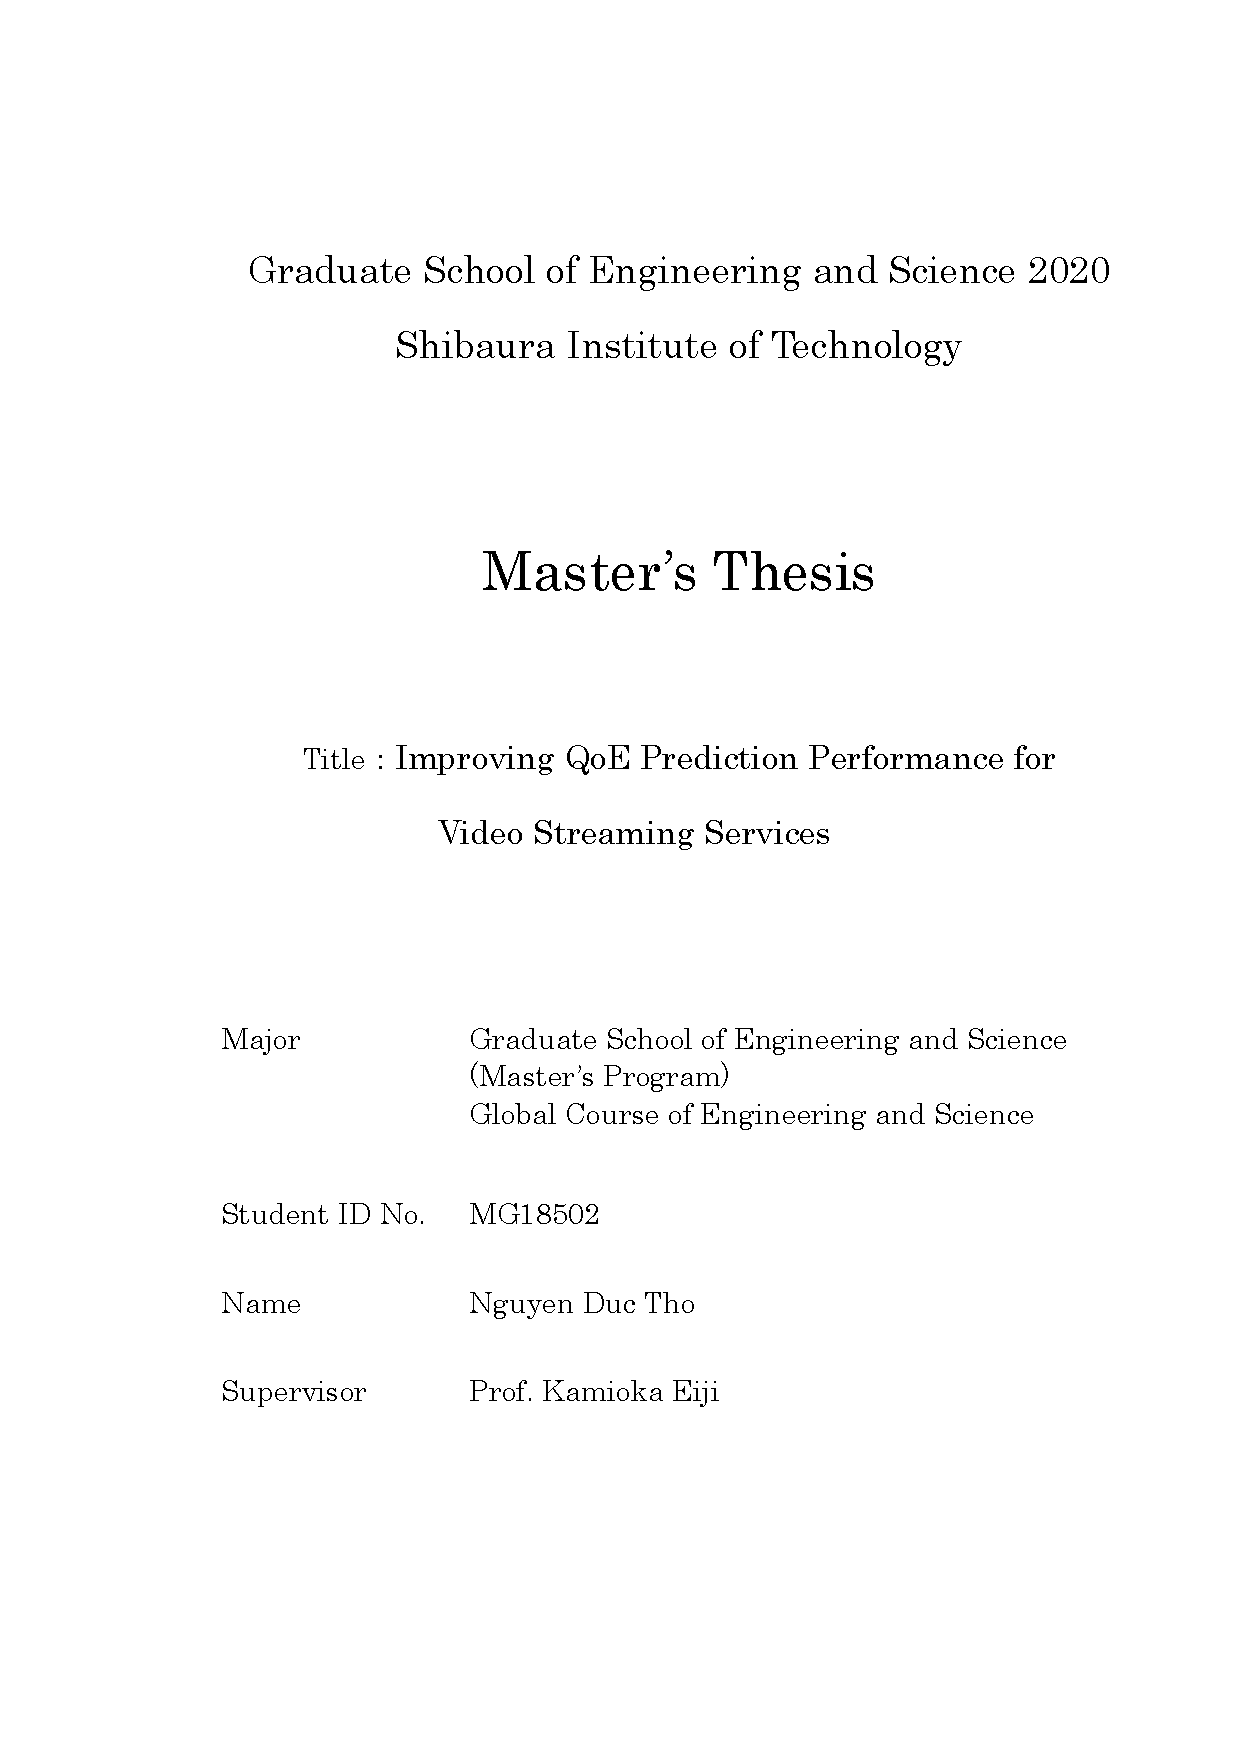
\includepdf[pages=-]{thesis-cover.pdf}

% % ******************************* Thesis Dedidcation ********************************

\begin{dedication} 

I would like to dedicate this thesis to my loving parents and my little brother \dots

\end{dedication}


\begin{declaration}


I hereby declare that except where specific reference is made to the work of others, the contents of this thesis are original and have not been submitted in whole or in part for consideration for any other degree or qualification in this, or any other university.


\end{declaration}
\begin{acknowledgements}      

I would like to express deep and sincere gratitude to my supervisor, Prof. Kamioka Eiji, for the continuous help and indispensable guidance which led me to the completion of this thesis, for his patience and motivation.
\\

I would also like to thank Dr. Phan Xuan Tan, for inspiring and guiding me throughout my studies.
It would have been more difficult without his invaluable advice and suggestions.
\\

I would like to thank my family for their love and hard work to make it possible for me to complete this thesis.
I would like to especially thank my parent for being there for me always.
To my little brother, you have been my main inspiration during all these years.
\\

Last but not least, I have been very thankful to my friend, Tran Minh Chanh, for his support in brainstorming new ideas and encouragement to complete this thesis.


\end{acknowledgements}

\begin{abstract}

The growing demand on video streaming services increasingly motivates the development of reliable and accurate models for the assessment of the user's Quality of Experience (QoE) in real-time to deliver high-quality streaming content to the user.
However, the complexity caused by the temporal dependencies in sequential QoE data and the non-linear relationships among QoE influence factors has introduced challenges to continuous QoE prediction.
This thesis proposes three novels QoE prediction models in order to improve the QoE prediction performance in terms of prediction accuracy and computational complexity.


\begin{itemize}
  \item First, to enhance the QoE prediction accuracy, the BiLSTM-QoE model is proposed.
  The model utilizes a Bidirectional Long Short Term-Memory network for predicting the user's QoE.  
  
  \item Second, the CNN-QoE model is introduced.
  The model leverages advantages of the Convolutional Neural Network to overcome the computational complexity drawbacks of Long Short Term-Memory networks while improving QoE prediction accuracy.
  Based on a comprehensive evaluation, the CNN-QoE model provides a high QoE prediction performance and outperforms the existing approaches.
  
  \item Third, human-related factors have a significant influence on QoE and play a crucial role in QoE modeling.
  However, these factors were not considered in the BiLSTM-QoE and CNN-QoE model due to the lack of data on QoE influence factors.
  Therefore, in order to precisely model the user's QoE, the impact of the human-related factors, namely perceptual factors, memory effect, and the degree of interest is investigated.
  Based on the investigation, a novel QoE model is proposed that effectively incorporates those factors to reflect the user’s cumulative perception.
  Evaluation results indicate that the model performs excellently in predicting cumulative QoE at any moment within a streaming session.


\end{itemize}


\end{abstract}

% *********************** Adding TOC and List of Figures ***********************

\tableofcontents

\listoffigures

\listoftables

% \printnomenclature[space] space can be set as 2em between symbol and description
%\printnomenclature[3em]

\printnomenclature[5em]

% ******************************** Main Matter *********************************
\mainmatter

\chapter{Introduction}
\label{ch:Introduction}


\renewcommand{\SectionsDir}{Chapter1/Sections}
\renewcommand{\FigsDir}{Chapter1/Figs}
\renewcommand{\TablesDir}{Chapter1/Tables}


\section{Motivation}
In recent years, video streaming has become the most dominant contributor to global Internet traffic.
The Cisco Visual Networking Index forecasts an increase in video traffic, which is expected to reach 82\% by 2021, up from 73\% in 2016 \citep{CiscoIndex}.
The rapid increase of video streaming services creates an extremely huge profit for streaming service providers.
In the context of a highly competitive streaming service market, service providers such as YouTube, Netflix, or Amazon must improve and ensure a sufficient video quality to satisfy the user's expectation, resulting in high quality of experience (QoE).
However, video streaming services are frequently influenced by dynamic network conditions (e.g., throughput, available bandwidth) which can lead to distorted events (e.g., bitrate switching, rebuffering events).
These distorted events can negatively affect the user's satisfaction, resulting in the deterioration of the user's QoE.
The capability of continuously predicting and monitoring the user's QoE in real-time can help video streaming controllers perform a QoE-based network control and management to alleviate the QoE deterioration, resulting in higher overall levels of the user's QoE \citep{QABR_Chanh, QABR_DeepQ}.
Therefore, there is a need for developing reliable QoE prediction models in order to quickly and accurately determine the user's QoE.


However, the continuous prediction of QoE is challenging since the user's QoE is affected by many influence factors such as video quality, video content, bitrate switching, rebuffering, etc.
Moreover, in order to accurately predict the user's QoE, it needs to capture the complex temporal dependencies in sequential QoE data and the non-linear relationships among these QoE influence factors  \citep{EffectSizesOfInfluenceFactors, QoEModel_TimeVaryingSubjectiveQuality, QoEModel_TVQoE_ContinuousTimeQoE, NetflixQoE}.
Additionally, QoE prediction models have to adapt to the dynamic changes in network conditions in real-time.
Therefore, it is necessary to improve the prediction accuracy of QoE models that can perform consistently well across diverse scenarios of video streaming.
Furthermore, it is necessary to optimize the model computational complexity for real-time QoE monitoring.
These factors form the motivation for this thesis.


The main goal of the thesis is to improve the QoE prediction performance in terms of both prediction accuracy and computational complexity of QoE prediction models for QoE-based network control and management.

\section{Research Contributions}
Based on the main goal, the work present in the thesis resulted in three novel QoE prediction models.
These models are summarized as follows:


\begin{enumerate}
  \item A QoE prediction model, namely BiLSTM-QoE, is proposed for continuously predicting the user's QoE.
  The BiLSTM-QoE model utilizes Bidirectional Long Short-Term Memory networks to deal with the complex temporal dependencies in sequential QoE data.
  The evaluation results show that the BiLSTM-QoE model achieves promising performance in terms of accuracy compared with other referenced models.
  
  
  \item Despite the high accuracy of the BiLSTM-QoE model, the sequential processing characteristic in BiLSTM architecture increases the computational complexity of the model.
  Thus, the CNN-QoE model is presented to overcome the computational complexity drawbacks, while at the same time improve QoE prediction accuracy.
  Based on a comprehensive evaluation, the CNN-QoE model can provide a high QoE prediction performance that outperforms the existing approaches.
  
  
  \item The BiLSTM-QoE and CNN-QoE models focused on continuously predicting the instantaneous QoE which can provide the user's instant perceived video quality at a certain moment.
  However, in order to correctly determine the user's QoE for performing a QoE-based network control and management, it is necessary to produce a highly accurate QoE prediction either at any moment or at the end of a streaming session.
  Thus, the user's cumulative QoE can be potentially utilized as a better alternative than instantaneous QoE.
  The cumulative QoE is cumulatively estimated from the time when the viewer starts watching a streaming video content to any moment of the streaming session.
  A novel cumulative QoE prediction model is proposed that precisely assesses the user's cumulative perception.
  Moreover, in order to accurately model the user's cumulative QoE, the model also takes into account the human-related factors (i.e., memory effects, user's interest in the video content) which is not considered in the BiLSTM-QoE and CNN-QoE models.
  Evaluation results indicated that the model performs excellently in predicting cumulative QoE at any moment within a streaming session.
\end{enumerate}

\section{Thesis Organization}
The rest of this thesis is organized as follows:


\begin{itemize}
  \item Chapter \ref{ch:Background} provides a more detailed background on QoE in video streaming, QoE assessment methodologies, and the QoE influence factors that need to be considered in QoE modeling.
  It also covers the literature review of the methods used for measuring and modeling the user's QoE.
  
  
  \item Chapters \ref{ch:BiLSTM}, \ref{ch:CNN}, and \ref{ch:Cumulative} presents three novel QoE prediction models.
  The work presented in these chapters has been published in \citep{Mine_BiLSTM}, \citep{Mine_CNN}, and \citep{ Mine_Cumulative}.
  

  \item After the three models have been presented, Chapter \ref{ch:Discussion} discusses the feasibility to utilize these models for QoE-based network control and management in video streaming.
  

  \item Chapter \ref{ch:Conclusion} concludes the thesis and shows potential future research work.
\end{itemize}


\nomenclature[z-QoE]{QoE}{Quality of Experience}
\nomenclature[z-BiLSTM]{BiLSTM}{Bidirectional Long Short-Term Memory}
\nomenclature[z-LSTM]{LSTM}{Long Short-Term Memory}
\nomenclature[z-CNN]{CNN}{Convolutional Neural Network}
\nomenclature[z-TCN]{TCN}{Temporal Convolutional Network}
\nomenclature[z-MOS]{MOS}{Mean Opinion Score}
\nomenclature[z-RMSE]{RMSE}{Root Mean Squared Error}
\nomenclature[z-PCC]{PCC}{Pearson Pearson Correlation Coefficient}
\nomenclature[z-SROCC]{SROCC}{Spearman Rank Correlation Coefficient}
% \nomenclature[e-HAS]{HAS}{HTTP Adaptive Streaming}
\chapter{Background and Literature Review}
\label{ch:Background}


\renewcommand{\SectionsDir}{Chapter2/Sections}
\renewcommand{\FigsDir}{Chapter2/Figs}
\renewcommand{\TablesDir}{Chapter2/Tables}


This chapter provides the necessary background on QoE, its assessment methods, and the QoE influence factors in video streaming.
It also presents the literature review of the approaches used for modeling the user's QoE.


\section{QoE Definition}
The definition of QoE proposed by European Network on QoE in Multimedia Systems and Service (the EU Qualinet community) is:
"QoE is the degree of delight or annoyance of the user of an application or service.
It results from the fulfillment of his or her expectations with respect to the utility and/or enjoyment of the application or service in the light of the user's personality and current state" \cite{QoEDef_Qualinet, QoEDef_ITU}.
This definition has pointed out that QoE is a user-centric metric used to measure the user's satisfaction with a particular service and their perception of the service's quality.

\section{QoE Assessment}
In order to improve and monitor the user's QoE, video streaming service providers have to develop various techniques to measure the QoE.
These techniques assess the user's QoE and quantify it in measurable metrics.
The user's QoE can be assessed both subjectively and objectively.


Subjective QoE assessment involves users and requires user surveys to gather subjective evaluations of a given service.
The most common method to capture subjective QoE evaluations is Mean Opinion Score (MOS) which is an ITU standardized \citep{QoEAss_ITU}.
MOS is a 5-point scale ranging from 1 to 5, which correlates to bad, poor, fair, good, and excellent.
Despite the high accuracy of the subjective assessment, it does have certain disadvantages. Firstly, a large number of participants need to be gathered in order to conduct the surveys. Secondly, this method is generally expensive in terms of cost and time consumption. Finally, it cannot be used for real-time QoE measurement or monitoring for video streaming.


Alternatively, objective QoE assessment is the most frequently used technique since it can be used to estimate the user's QoE without requiring human interaction.
Objective QoE models are more suited for real-time QoE measurements. However, it can be less accurate than subjective QoE evaluations.

\section{QoE Influence Factors}
The user's QoE in video streaming is affected by multiple factors.
These factors can be classified into the following four categories \citep{Survey_QoEModeling, EffectSizesOfInfluenceFactors}:


\begin{enumerate}
  \item \textbf{System-related Influence Factors}
  consider the technical aspects of video streaming quality.
  They include the influences of the user device (e.g., computing power, screen size), network-related (e.g., bandwidth, delay), and also the application layer (e.g., video adaptation strategy, rebuffering events, bitrate switching events).


  \item \textbf{Human-related Influence Factors}
  are related to the user's information and characteristic.
  They include psychological factors of the user such as user expectations, memory and recency effects, or user's background and usage history.
  
  
  \item \textbf{Context-related Influence Factors}
  capture the environment and the context where the user views the video content.
  They address the user's location and space, subscription type, time of the day, the purpose of viewing the video, etc.
  
  
  \item \textbf{Content-related Influence Factors}
  consider the characteristics of the video content.
  They include the influence of encoding rate, encoding format, resolution, playback duration, type of video, etc.
\end{enumerate}

\section{Literature Review on QoE Modeling}
QoE modeling for video streaming services has received enormous attention due to its critical importance in QoE-aware applications.
A number of different continuous QoE prediction models have been proposed \cite{QoEModel_TimeVaryingSubjectiveQuality, QoeModel_ShortLongTermQualityModel, QoEModel_BitrateDistribution, QoEModel_NARX_DynamicNetworks, QoEModel_AugmentedAutoregressive, QoEModel_TVQoE_ContinuousTimeQoE, QoEModel_NLSS, QoEModel_3D, QoEModel_Wireless}.
The authors in \cite{QoEModel_TimeVaryingSubjectiveQuality} modeled the time-varying subjective quality (TVSQ) using a Hammerstein-Wiener model.
The work in \cite{QoEModel_AugmentedAutoregressive} proposed a model based on the augmented Nonlinear Autoregressive Network with Exogenous Inputs (NARX) for continuous QoE prediction.
It should be noted that these models did not consider rebuffering events which usually happen in video streaming \cite{Survey_QoE, Survey_QoEModeling}.
On the other hand, the study in \cite{QoEModel_NARX_DynamicNetworks} took into account rebuffering events, perceptual video quality, and memory-related features for QoE prediction.
However, the QoE prediction accuracy varied across different video streaming scenarios.
The reason is that the model suffered from the difficulty in capturing the complex dependencies among QoE influence factors, leading to unreliable and unstable QoE prediction performances.


In order to address the above challenges, the authors in \cite{QoEModel_LSTM} proposed a QoE prediction model, namely, LSTM-QoE, which was based on Long Short-Term Memory networks (LSTM).
The authors argued that the continuous QoE is dynamic and time-varying in response to QoE influencing events such as rebuffering \cite{MeasuringQoEOfHTTP} and bitrate adaptation \cite{QoEModel_TimeVaryingSubjectiveQuality}.
To capture such dynamics, LSTM was employed and the effectiveness in modeling the complex temporal dependencies in sequential QoE data was shown.
The model was evaluated on different QoE databases and outperformed the existing models in terms of QoE prediction accuracy.
However, the computational complexity of the model was not fully inspected.
Since the recurrent structure in LSTM can only process the task sequentially, the model failed to effectively utilize the parallel computing power of modern computers, leading to a high computational cost.
Therefore, the feasibility to utilize the LSTM-QoE model for real-time video streaming applications remains an open question.


Therefore, in this thesis, we aim to improve the QoE prediction performance of QoE prediction models by enhancing the QoE prediction accuracy and optimizing the computational complexity.

\chapter{BiLSTM-QoE Model}
\label{ch:BiLSTM}


\renewcommand{\SectionsDir}{Chapter3/Sections}
\renewcommand{\FigsDir}{Chapter3/Figs}
\renewcommand{\TablesDir}{Chapter3/Tables}


\section{Introduction}
\label{BiLSTM:sec:Introduction}
Most of existing works only focused on modeling the overall or the instantaneous QoE, which have shown insufficient characteristics.
The overall QoE \cite{QoEModel_OP_EstimatingQoE, QoEModel_OP_DerivingValidatingUserExperience, QoEModel_OP_VideoQualityMetric}, which demonstrates the final subjective judgment for a streaming session, can only be assessed when the viewer finishes watching.
Therefore, the overall QoE cannot be applied for real-time QoE monitor and also does not give sufficient information about events occurring during the session.
Although the instantaneous QoE \cite{QoEModel_TimeVaryingSubjectiveQuality, QoeModel_ShortLongTermQualityModel}, on the other hand, can provide the instant perceived video quality at a certain moment, it only reflects locally the quality assessment within a specific time range, without considering the cumulative effects of prior events.
Hence, it is highly sensitive to video impairments due to hysteresis effect \cite{TemporalHysteresisModel, StallingEvents} and does not precisely express the user's perceived video quality.
In contrast, modeling and predicting the user's cumulative perception to a streaming video content are able to provide lots of advantages for QoE monitor and control systems since it not only reflects the user's overall satisfaction but also reveals the impact of distorted events happening during the streaming session.



In addition, according to \citep{QoEDef_Qualinet}, QoE is defined as the results from the fulfillment of the user's expectation to the enjoyment of the application or service based on his or her \textit{personality} and \textit{current state}.
Here, "personality" defines "the characteristics of a person that account for consistent patterns of feeling, thinking and behaving", whereas, "current state" stands for "situational or temporal changes in the feeling, thinking or behavior of a person".
Therefore, human-related influence factors (e.g., perceptual factors, memory effect, user's interest in video content) play a crucial role in accurately modeling the user's QoE.


Some studies investigate and quantify the impact of perceptual factors \cite{QoEModel_OP_EstimatingQoE, QoEModel_OP_DerivingValidatingUserExperience, QoEModel_OP_VideoQualityMetric, QoEModel_TimeVaryingSubjectiveQuality, QoeModel_ShortLongTermQualityModel}.
However, the authors usually abandon the temporal dynamics and historical experience of the user's satisfaction, which are referred to as the memory effects \cite{MemoryEffects_WebQoE}.
Some other studies attempt to clarify the role of primacy and recency effects \cite{QoEModel_BitrateDistribution, QoEModel_OM_DistortionsRebuffMemory, QoEModel_NARX_DynamicNetworks, LFOVIA, QoEModel_TVQoE_ContinuousTimeQoE, QoEModel_NLSS, QoEModel_LSTM}, resulting in the high accurate QoE prediction.
Typically, the primacy and recency effects \cite{PrimacyVsRecency} determine the memory influence of impairments occurring at the beginning and the end of streaming session \cite{NetflixQoE}, respectively.
Besides, the effect of unpleasant events which take place in the middle of the session also leaves a considerable impact on the perceived video quality \cite{NetflixQoE,StallingEvents}.
Theoretically, such impacts can be represented by an exponential deterioration of memory retention in time (defined by \textit{forgetting curve}) \cite{UserForgetful, EvaluatingForgettingCurves, Ebbinghaus_ForgettingCurve} for infrequent events or by \textit{repetition} \cite{StallingEvents, Ebbinghaus_ForgettingCurve} for the repeated impairments.
However, the influence of forgetting behavior and repetition has not been carefully investigated in existing QoE models.
Therefore, to fully express human memory effects on QoE assessment, in addition to the primacy and recency effects, the forgetting curve and repetition should be involved in the discussion.


Apart from that, the factors that relate to video content also have a noticeable effect on perceived QoE. Those factors might be type of video, video complexity \cite{EffectSizesOfInfluenceFactors}, etc.
Additionally, some studies (e.g., \cite{QoSImpactUserVideoClips, SubjectiveQualityPairedComparison, QoEEvaluation_IPTV_Services}) have found that the user's interest in video content possibly generates the bias in his/her QoE evaluation.
More concretely, the user tends to provide higher QoE scores for more attractive video contents.
Such a behavior is influenced by the so-called degree of interest (DoI) which clarifies the interestingness of different video content, or the ability of the video content to attract the user and keep the user's interest \cite{VisualContent}.
However, existing studies often neglect this factor due to the fact that these numerical values might vary upon different users based on their personal interests.


For those reasons, in this chapter, we present a cumulative QoE model that extremely well quantifies multiple effects of human-related factors, that is to say, perceptual influence factors, memory effect and degree of interest (DoI).
In order to assess the accuracy in predicting cumulative QoE, the cumulative QoE model is evaluated over LFOVIA database \cite{LFOVIA} and through the subjective evaluation.
Evaluation results demonstrate that the cumulative QoE at different moments within a streaming session is precisely predicted by the model.
It shows the potential of cumulative QoE that can be utilized as a better alternative than either overall QoE or instantaneous QoE in QoE monitoring and management.

The rest of this chapter is organized as follows.
Section \ref{Cumulative:sec:Proposals} investigates the influence of human-related factors and presents the cumulative QoE prediction model.
 Section \ref{Cumulative:sec:Evaluation} evaluates the performance of the proposal and discusses the advantages and disadvantages.
 Section \ref{Cumulative:sec:Summary} summarizes this chapter.

\section{Model Architecture}
\label{BiLSTM:sec:Proposals}
In this section, we first investigate the impact of those factors on human perception in QoE evaluation and then formulate the proposed cumulative QoE model.

\subsection{Perceptual factors} \label{section:PerceptualFactors}
In video QoE assessment, perceptual factors \citep{Survey_QoE} including video quality, rebuffering frequency, rebuffering duration are directly perceived by the user.
Sub-section \ref{BiLSTM:subsec:InputFeatures} has introduced four input features (i.e. STSQ, PI, NR, and TR) that are related to perceptual factors.
These input features are fed into an LSTM-QoE model \citep{QoEModel_LSTM} to predict the instantaneous QoE as follows \citep{QoEModel_LSTM}:

\begin{equation}
    q(t) = LSTM^{0}(\bm{x}(t), \bm{c}(t-1))
\end{equation}
where, $q(t)$ represents the predicted instantaneous QoE at the time instant $t$, $\bm{x}(t)$ is the input features, $\bm{c}(t)$ is the memory cells which encode the knowledge of the inputs that have been observed up to the time $t$. $LSTM$ provides two functionalities: $LSTM^{0}$ for output QoE prediction and $LSTM^{c}$ for memory cells update which is given by  \citep{QoEModel_LSTM}:

\begin{equation}
    \bm{c}(t) = LSTM^{c}(\bm{c}(0:t-1), q(0:t-1)), \forall t \ge 1
\end{equation}

where, $\bm{c}(0:t-1)$ and $q(0:t-1)$ respectively refer to the past memory cells and the past predicted QoE.


The architecture of LSTM-QoE model are illustrated in Figure \ref{fig:LSTM}.

\begin{figure}[tb]
  \begin{center}
    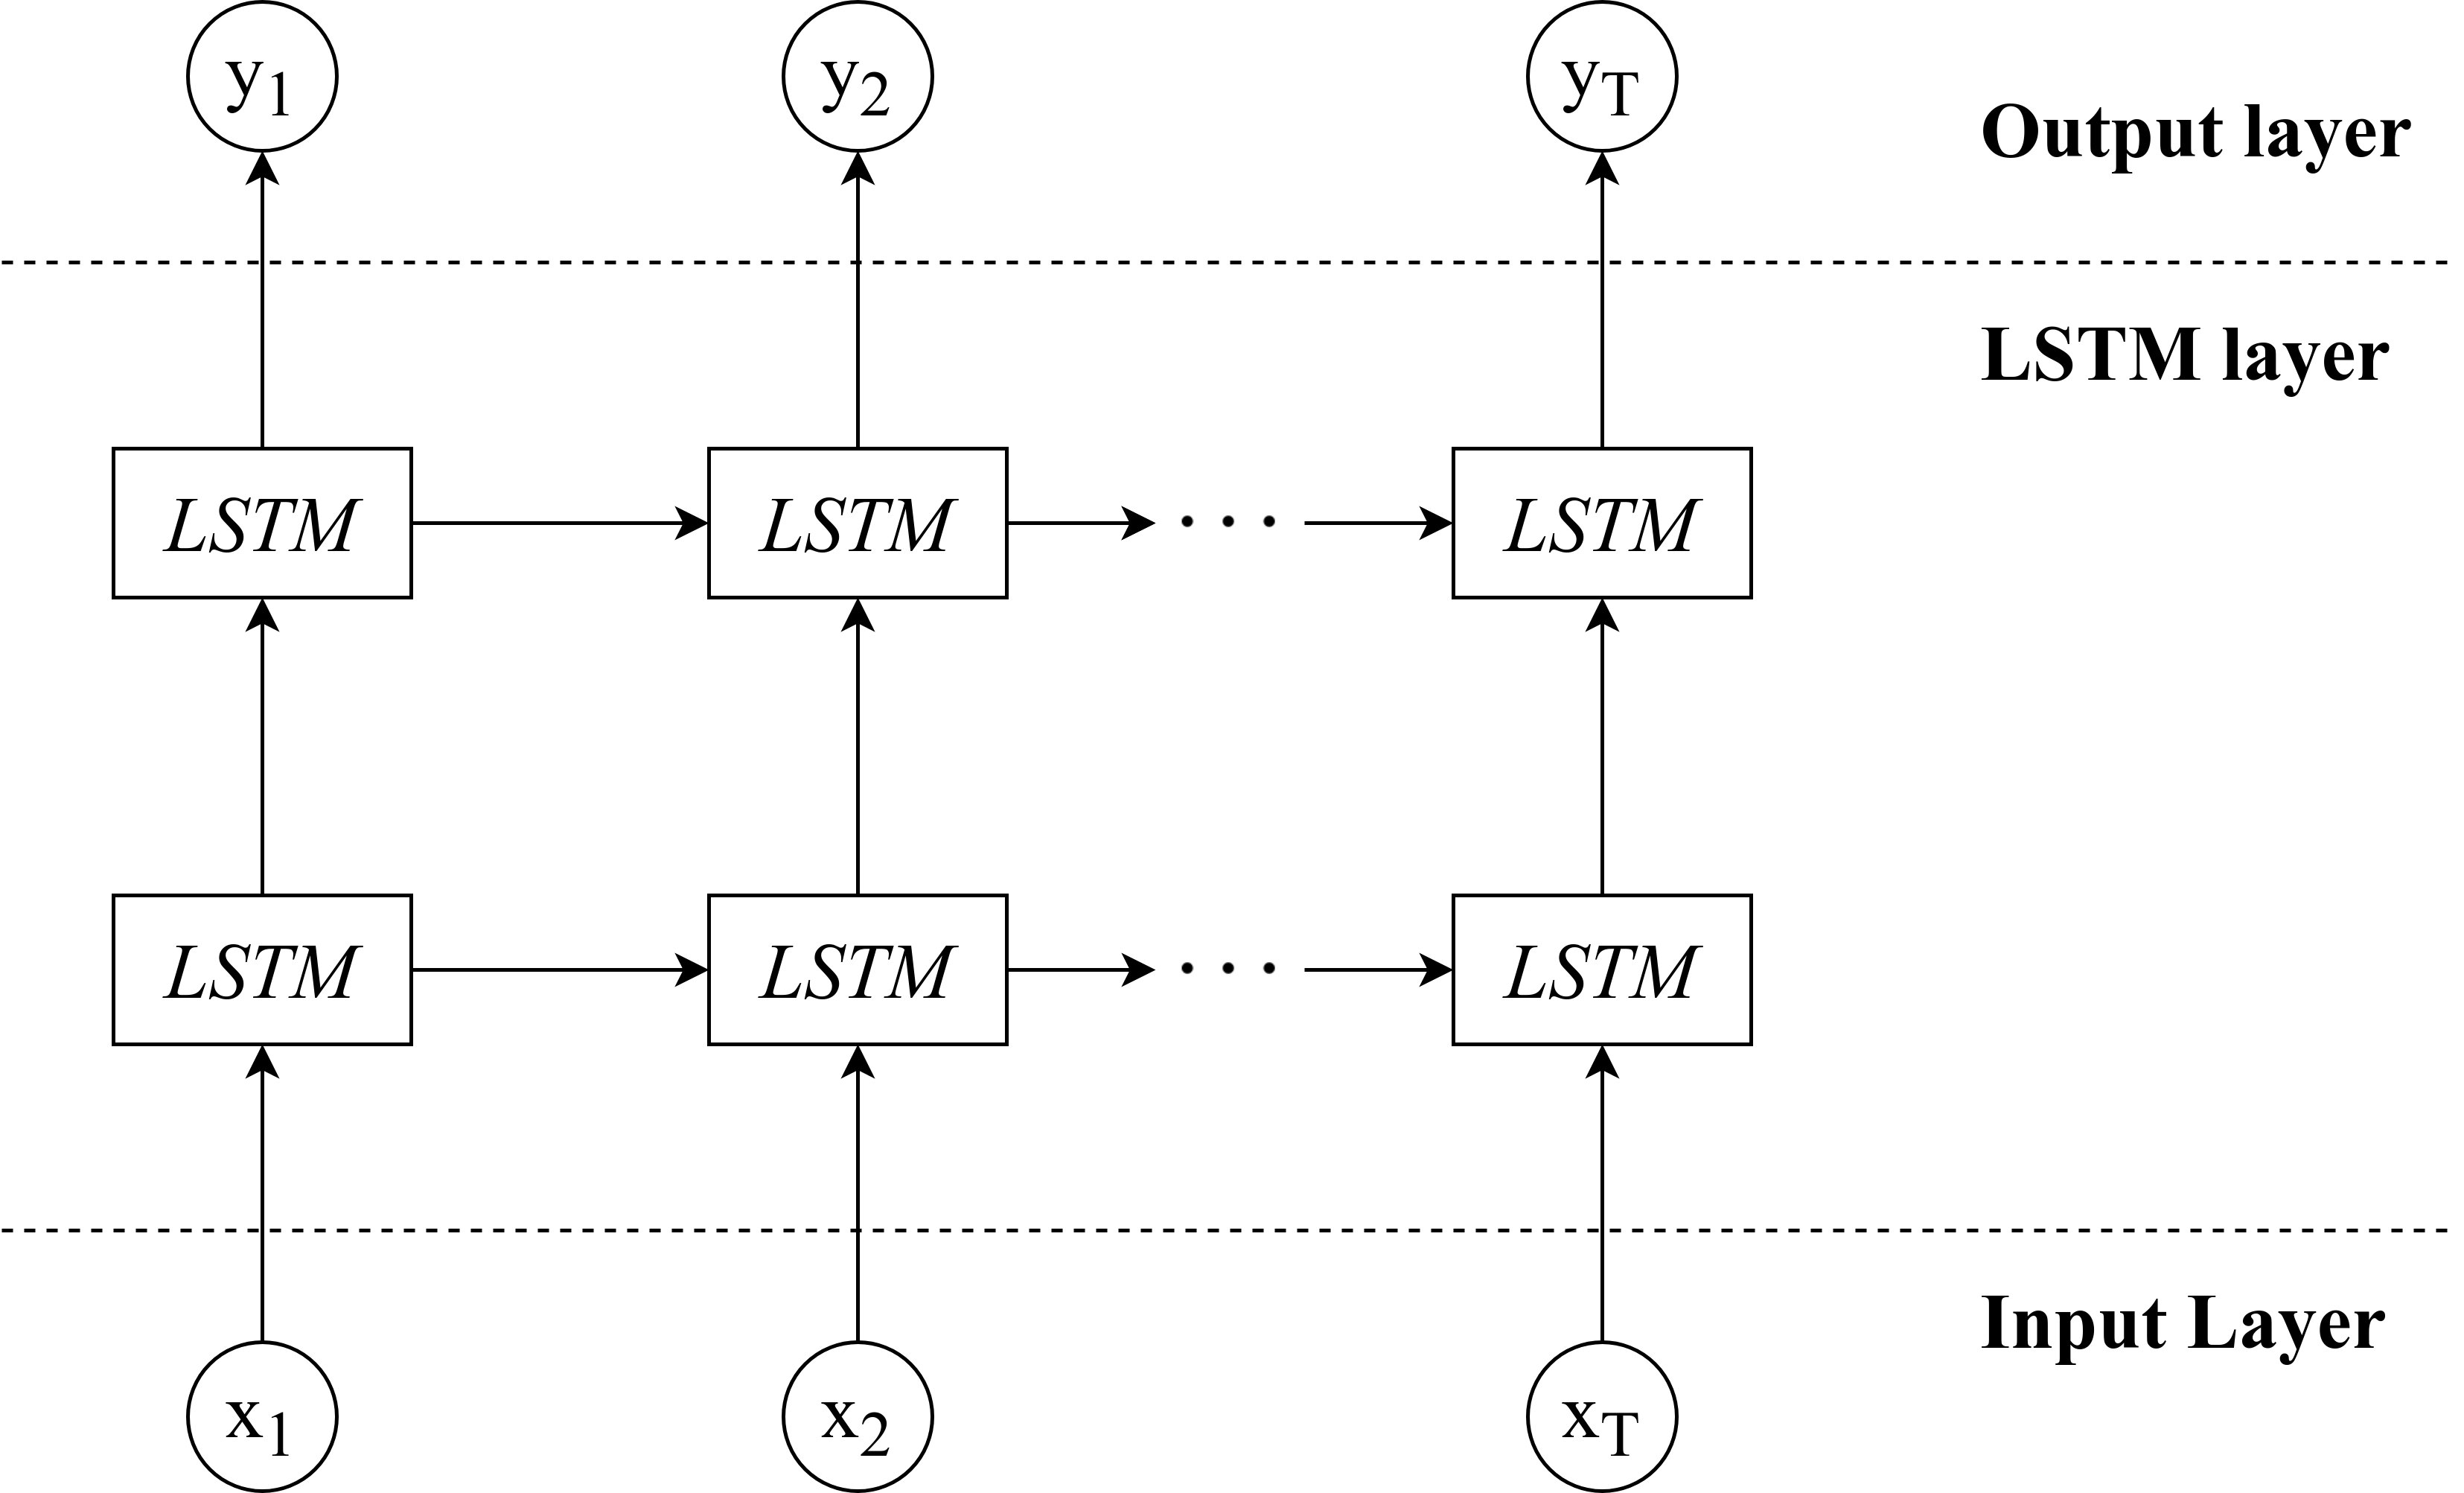
\includegraphics[width=0.6\linewidth]{\FigsDir/LSTM.png}
  \end{center}
  \caption{LSTM network \citep{QoEModel_LSTM} for the user's instantaneous QoE prediction. The network is composed of two LSTM (Long Short-term Memory) layers. The inputs to the layers are four features including STSQ, PI, NR, and TR. The outputs combine the LSTM layers' hidden states, representing the predicted instantaneous QoE values.}
  \label{fig:LSTM}
\end{figure}

\subsection{Memory Effects} \label{section:MemoryEffects}
Memory effects refer to the influence of historical/past experiences on the perceived video quality. Primacy and recency are two common effects which were investigated in numerous studies \cite{QoEModel_LSTM, QoEModel_TVQoE_ContinuousTimeQoE, QoEModel_NARX_DynamicNetworks}. In addition to these factors, the effect of forgetting curve characteristic and repetition are also considered in our proposed model.
%for the improvement of accuracy
The next parts of this subsection will discuss the role and mathematical function of these factors. Based on that, a memory weight is proposed for the cumulative QoE model.

%/====================================================================================
\subsubsection{Primacy Effect}
%/====================================================================================

The primacy effect \cite{SerialPositionEffect_FreeRecall, PrimacyVsRecency} describes the human behavior to recall (bitrate or rebuffering) initial events occurred at the beginning of the streaming session when providing the overall evaluation \cite{RehearsalProcessesInFreeRecall}. In fact, the primacy effect always exponentially decreases by time \cite{SerialPositionEffect_FreeRecall}. Therefore, its characteristics can be expressed by an exponential curve as follows:
    
\begin{equation} \label{eqn:Primacy}
  f_{P}(t) = exp(-\alpha_{P}*t), \quad 0 \leq t \leq L
\end{equation}
where $\alpha_{P}$ determines the \textit{intensity} of primacy effect (how fast the primacy effect diminishes over time) and $t$ denotes a time instant within a session of $L$ seconds.


%/====================================================================================
\subsubsection{Recency Effect}
%/====================================================================================

The recency effect \cite{SerialPositionEffect_FreeRecall,PrimacyVsRecency} refers to the ability of the human memory to recall the most recent events \cite{RehearsalProcessesInFreeRecall}, hence, the evaluated QoE heavily depends on the recent experiences. The recency effect also can be described by an exponential curve represented by the following equation:
    
\begin{equation} \label{eqn:Recency}
  f_{R}(t) = exp(-\alpha_{R}*(L - t)), \quad 0 \leq t \leq L
\end{equation}
where $\alpha_{R}$ determines the \textit{intensity} of recency effect.
    
The primacy effect and the recency effect can be combined as the U-shaped form \cite{PrimacyVsRecency}, quantifying the influenced weight of the events occurring from the beginning to the end of a video session. As shown in Figure\,\ref{fig:PrimacyRecencyShape}, it can be observed that both Eq. \ref{eqn:Primacy} and Eq. \ref{eqn:Recency} reflect the primacy and recency effect extremely well.
    
\begin{figure}[tb]
  \begin{center}
    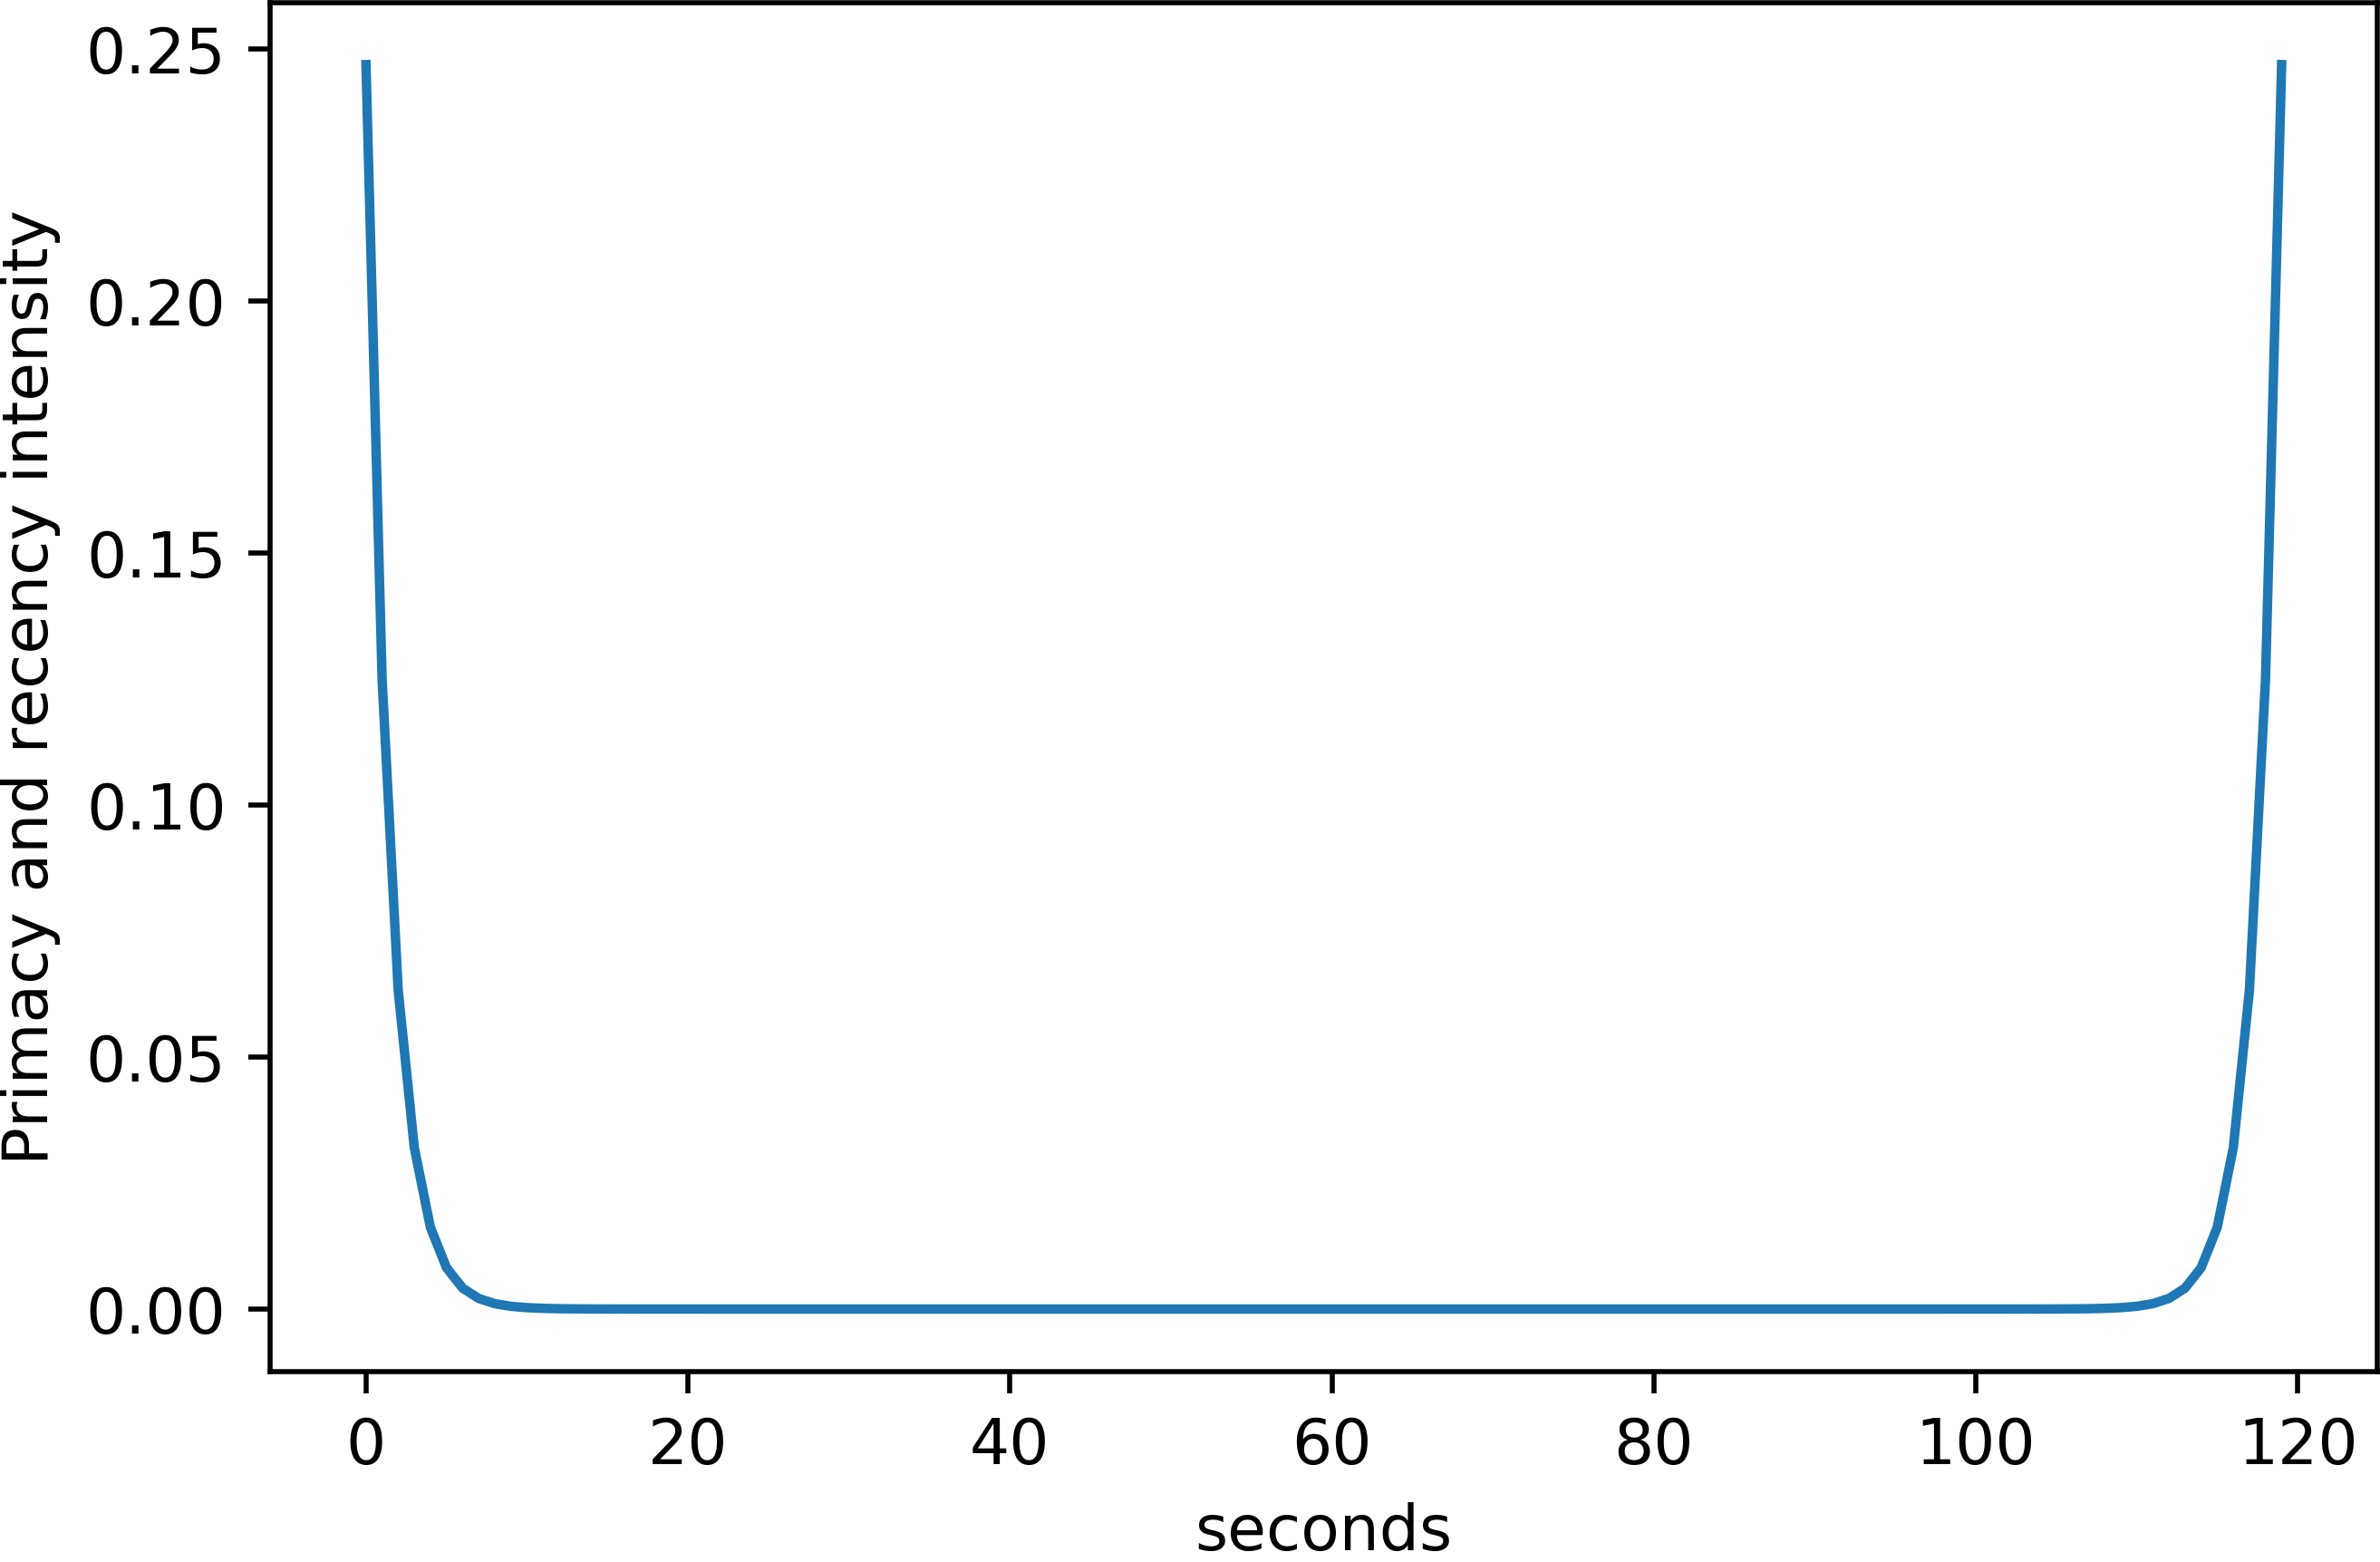
\includegraphics[width=0.6\linewidth]{\FigsDir/weight_ideal.png}
  \end{center} 
  \caption{A typical U-shaped curve combined primacy and recency effects.}
  \label{fig:PrimacyRecencyShape}
\end{figure}


%/====================================================================================
\subsubsection{Forgetting Curve and Repetition}\label{pro_for-rep}
%/====================================================================================

\begin{figure}[tb]
  \centering
  \begin{subfigure}[b]{0.49\linewidth}
    \centering
    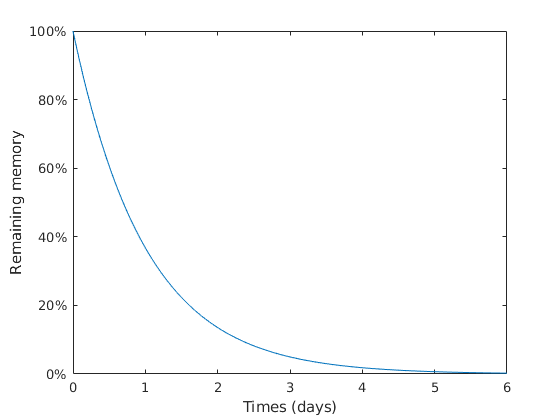
\includegraphics[width=\linewidth]{\FigsDir/forgetting_curve.png}
    \caption{An example of forgetting curve}
    \label{fig:ForgettingCurve}
  \end{subfigure}
  \hfill
  \begin{subfigure}[b]{0.49\linewidth}
    \centering
    \includegraphics[width=\linewidth]{\FigsDir/repetition_redraw.png}
    \caption{Forgetting curve and repetition}
    \label{fig:ForgettingCurveRepetition}
  \end{subfigure}
  
  \caption{Examples of forgetting curve and repetition.}
  \label{fig:ForgettingCurveRepetitionExamples}
\end{figure}

%Human memory is complex; thus, 
Due to the significant impact of the negative experience caused by distorted events, the primacy and recency effect can be neglected under repeated bitrate switches or rebuffering \cite{EffectSizesOfInfluenceFactors}. In such situations, forgetting behavior and repetition should be taken into account. The forgetting behavior, in other words, forgetting curve characteristic \cite{Ebbinghaus_ForgettingCurve} is a natural process, describing the exponential loss of memory over time. As shown in Figure \ref{fig:ForgettingCurve}, when information is learned, its memory retention declines at an exponential rate. Accordingly, any occurred events can be exponentially forgotten by time if there is no attempt to retain it. The level of remaining memory about such events at a specific time point depends on:

\begin{itemize}
  \item The strength of memory (memory intensity): The durability that memory traces in the brain. The more annoyance the event is, the stronger the user memorizes it and the longer it lasts.
  \item The time has elapsed since the occurrences of events: As shown in Figure\,\ref{fig:ForgettingCurve}, the user will forget an average of 60\% of what they experience within the first period of time \cite{EvaluatingForgettingCurves,Ebbinghaus_ForgettingCurve}.
  \item Repetition: The more frequently an event occurs, the more likely it sticks to the user memory (shown in Figure\,\ref{fig:ForgettingCurveRepetition})
\end{itemize}

In a typical streaming session, an interruption (bitrate switching or rebuffering) can happen regularly. When an event, especially rebuffering repeatedly occurs, the strength of memory of those events will trendily increases \cite{Ebbinghaus_ForgettingCurve}, negatively influencing the perceived video quality. Consequently, as the number of negative events increases, QoE will recover at a slower pace after the occurrence of each event. Such memory characteristics can be formulated as the following equation \cite{TwoComponentsOfMemory}:
    
\begin{equation} \label{eqn:Repetition}
  f_{RP}(t) = exp(-\frac{\alpha_{RP}}{NR(t)} * TR(t)), \quad 0 \leq t \leq L
\end{equation}
where $NR(t)$ is the number of rebuffering events occurring until the time $t$, $TR(t)$ is the time elapsed since the last video impairment, and $\alpha_{RP}$ is the intensity of memory related to a rebuffering event. The ratio $\frac{\alpha_{RP}}{NR(t)}$ determines the retention of the user's memory after the $NR(t)$-th rebuffering. Accordingly, the lower $\frac{\alpha_{RP}}{NR(t)}$ is, the higher retention rate, making $f_{RP}$ declines at a lower rate. 


%/====================================================================================
\subsubsection{Proposed Memory Weight}
%/====================================================================================

As discussed in the previous sub-subsections, the effects of primacy, recency, forgetting behavior and repetition are significantly crucial for the evaluation of the cumulative QoE. Therefore, in the proposed cumulative QoE model, we introduce a novel \textit{memory weight} incorporating the effects of those factors to accurately assess the cumulative human perception during a streaming session. The proposed memory weight is represented by Eq. \ref{eqn:Weight}. An example of time-varying memory weight is illustrated in Figure \ref{fig:ForgettingCurveRebuff}. In fact, Eq. \ref{eqn:Weight} is a linear combination effect of the above-mentioned memory factors obtained from Eq. \ref{eqn:Primacy}, Eq. \ref{eqn:Recency} and Eq. \ref{eqn:Repetition}.
    
\begin{equation} \label{eqn:Weight}
  w_{t} = \beta_{1}f_{P}(t) + \beta_{2}f_{R}(t) + \beta_{3}f_{RP}(t)
\end{equation}

\begin{figure}[tb]
  \begin{center}
    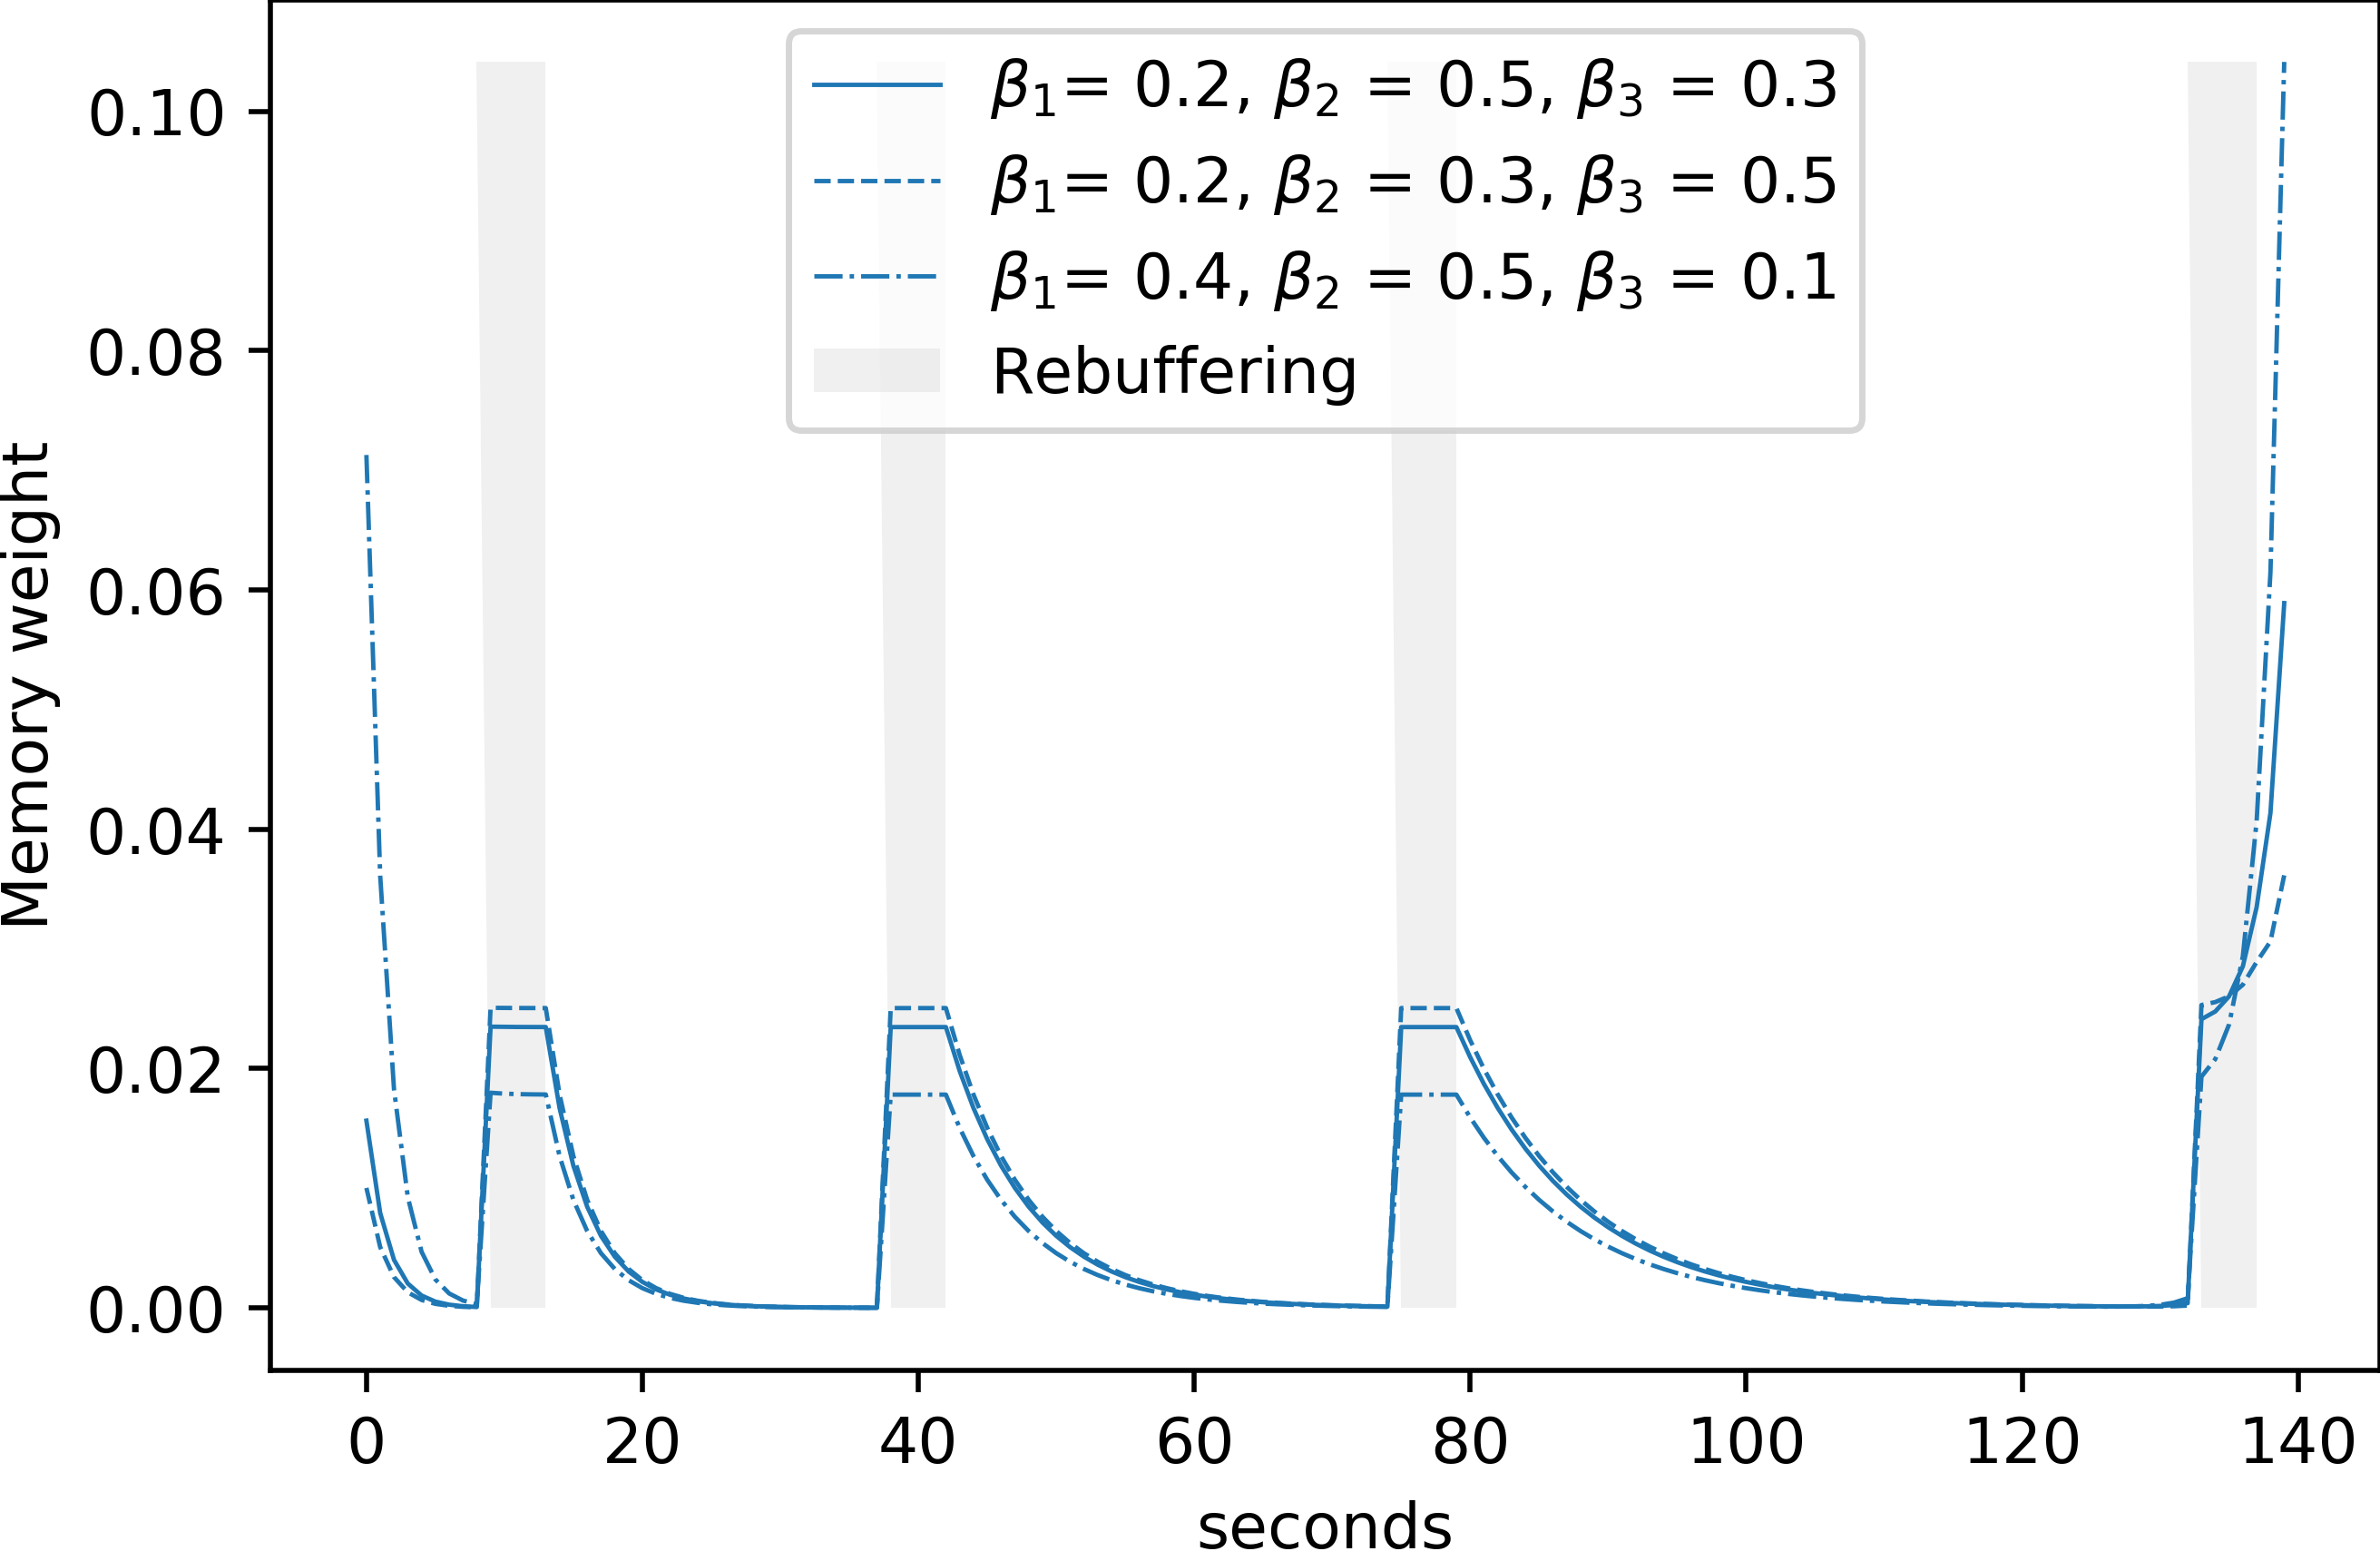
\includegraphics[width=0.7\linewidth]{\FigsDir/weight_different_params.png}
  \end{center} 
  \caption{An example of the memory weight in a session under different values of parameters $\beta_{1}$, $\beta_{2}$, and $\beta_{3}$}
  \label{fig:ForgettingCurveRebuff}
\end{figure}


where $\beta_{1},\beta_{2},\beta_{3}$ respectively determine the contribution of primacy effect, recency effect and repetition to the memory weight.

Figure. \ref{fig:ForgettingCurveRebuff} shows that when an rebuffering event occurs near the end of the session, the recency effect has a stronger effect on human perception. Therefore, in this period of times, the end user's QoE will drops dramatically. In addition, the forgetting rate of a specific interruption is also smaller than those of previous ones, determining the characteristics of forgetting behavior and repetition. Therefore, the proposed memory weight potentially reflects the intensity of human memory over time during a streaming session.


\subsection{Degree-of-Interest} \label{section:DoI}
For modeling QoE, there have been numerous studies that take into account video content-related factors (e.g., type of video, the complexity of video, etc.). However, most of them neglected the user's interest, in other words, DoI. In fact, influenced by video content and viewer preferences, the user possibly has different DoI on different videos or different parts of a video. Intuitively, the user seems to provide higher QoE scores for the video with interesting content and vice versa. Typically, Degree-of-Interest (DoI) \cite{DegreeOfLiking_SOS} is defined as the interestingness of the video content, or the ability of the video content to attract the user and keep the user's interest \cite{VisualContent}.

To make this clear, we investigate the correlation between DoI and the overall QoE by conducting a subjective test. In this test, 18 undistorted videos from the LFOVIA Database \cite{LFOVIA} were utilized. The video content varied upon nature, wildlife, outdoor, marine, sports, animation, and gaming \cite{LFOVIA} among every video, each of which the duration is 120 seconds. This guaranteed that the subjects would retain their interests as they watched.
%The snapshots of these videos are shown in Figure \ref{fig:snapshots}.
The referenced videos were randomly divided into 6 collections and encoded using FFmpeg \cite{FFmpeg} under the default settings with the resolution of 1920 x 1080 and were displayed on a 15-inch monitor with a resolution of 1920 x 1080 and a black background. The Absolute Category Rating (ACR) \cite{ITUT_P913} method was used and there were 60 subjects agreed to participate in this experiment. Each video was assessed by at least 10 subjects. At the end of each video, the subject was asked to give an overall score representing his/her interest in the entire video content, ranging from 1 (worst or not at all interested) to 5 (best or extremely interested), following the general principle of the ITU-T recommendation P.913 \cite{ITUT_P913}. A 3-minute break was provided to each subject between each video to minimize the effects of viewer fatigue. The average of subjects' scores or Mean Opinion Score (MOS) for each video was utilized as the DoI of video. These values were then linearly scaled up to the range of 0 to 100 and compared with the corresponding overall QoE in the LFOVIA Database.

\begin{figure}[tb]
  \begin{center}
    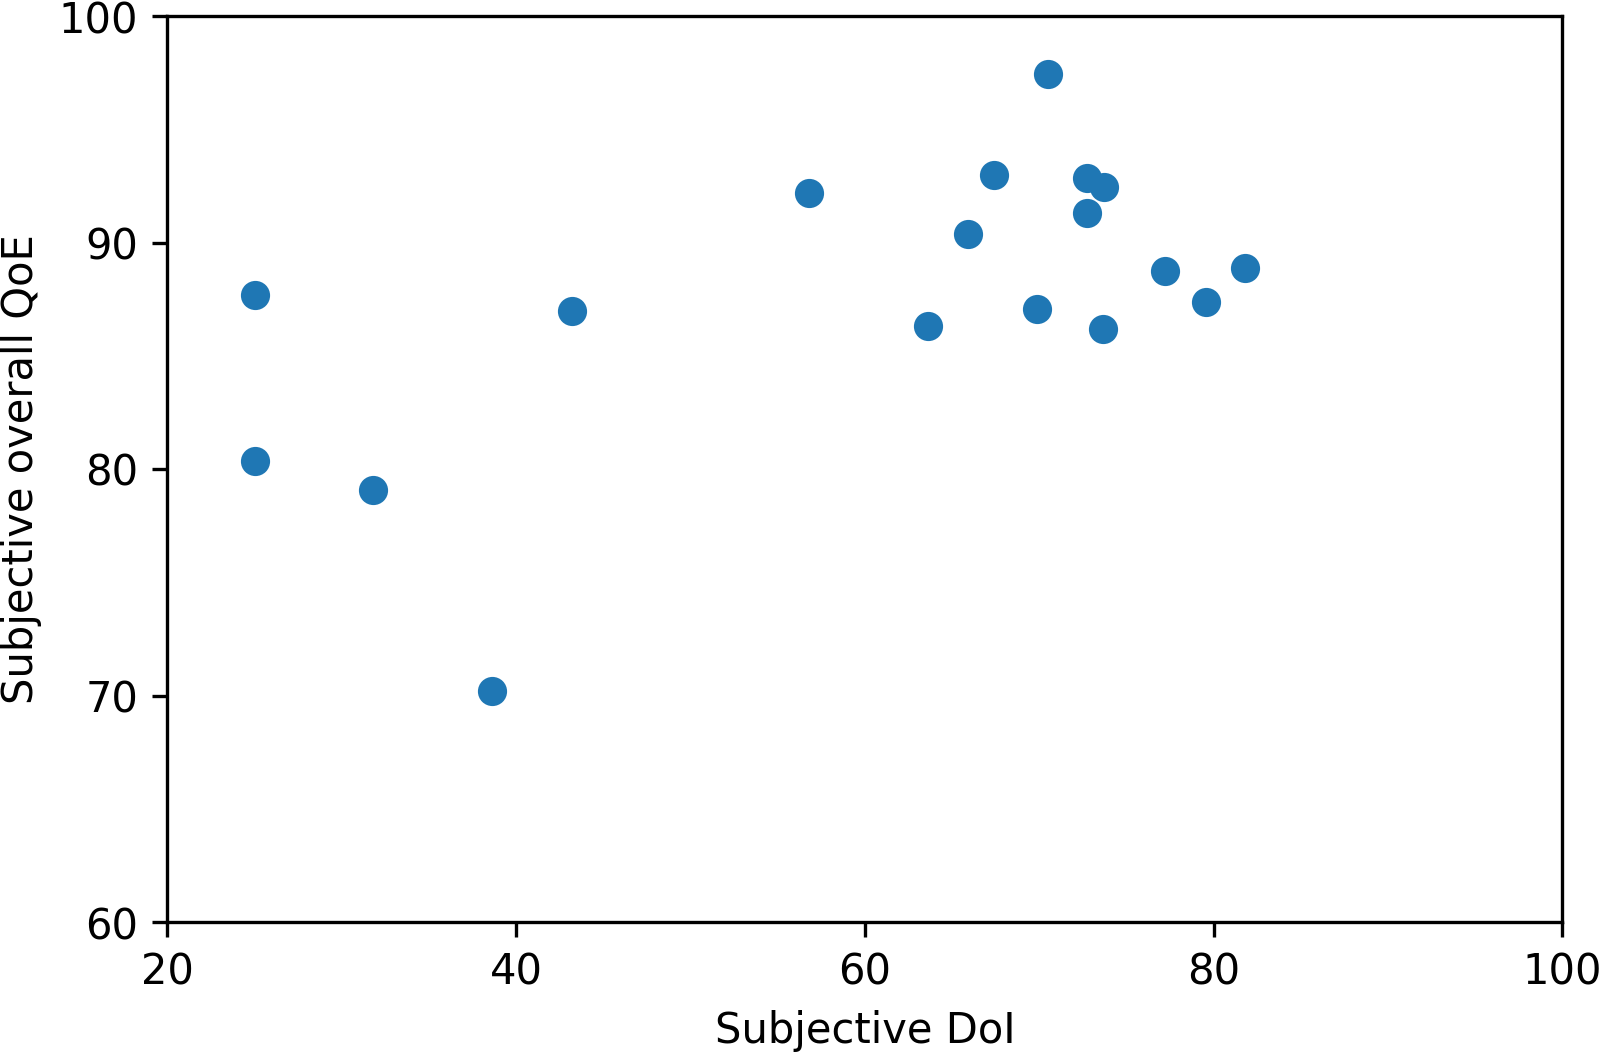
\includegraphics[width=0.6\linewidth]{\FigsDir/pcc_doi_overallqoe.png}
  \end{center}
  \caption{Scatter plot between the mean of subjective DoI scores and the subjective overall QoE obtained in the database.}
  \label{fig:PCC_DoI_OverallQoE}
\end{figure}

Figure \ref{fig:PCC_DoI_OverallQoE} illustrates the obtained correlation between DoI and the overall QoE, which achieved the Pearson Correlation Coefficient (PCC) of \textbf{0.601}. The correlation was modest. We speculate this as the small number of subjects participating in the experiment. Yet, it is shown that the DoI has an influence on the final decisions of the users when they provide the overall QoE. In the future, a larger number of subjects will be considered for further investigation. Based on the conclusion of this experiment, we introduce DoI as one of the potential influence factors in the proposed cumulative QoE model.


\subsection{Cumulative QoE model} \label{section:CumulativeQoE}
Through the investigation of the above human-related influence factors, the proposed cumulative QoE model is generally presented in Eq.\,\ref{eqn:Cumulative_QoE}. In this model,
to quantify how each of the user's past experiences influences the cumulative perception,
the instantaneous QoE needs to be weighted by the memory effect from the beginning of playback to the investigated time point $t$ within a streaming session.
According to our proposed model, the procedure of estimating cumulative QoE is described as follows: Firstly, the instantaneous QoE is predicted by LSTM-QoE model \cite{QoEModel_LSTM}, and stored into vector ${Q}_{t} = (q_{0},  q_{1}, \dots, q_{t})$. Secondly, the memory weight is calculated by the Eq.\,\ref{eqn:Weight} to form vector ${W}_{t} = (w_{0},  w_{1}, \dots, w_{t})$.

\begin{equation} \label{eqn:Cumulative_QoE}
  CQ_{t} = \lambda_{1} \left ( {Q}_{t}\times{W}^{T}_{t} \right ) + \lambda_{2}DoI
\end{equation}

where $\lambda_{1}$, $\lambda_{2}$ are correlation coefficients which respectively determine the contribution of the user's past experience and user's interest in video content to the predicted cumulative QoE $CQ_{t}$ at time instant $t$.


\section{Performance Evaluation}
\label{BiLSTM:sec:Evaluation}
\subsection{Input Features for QoE Prediction}
\label{BiLSTM:subsec:InputFeatures}


\begin{figure}[tb]
  \centering
  \begin{subfigure}{0.48\linewidth}
    \centering
    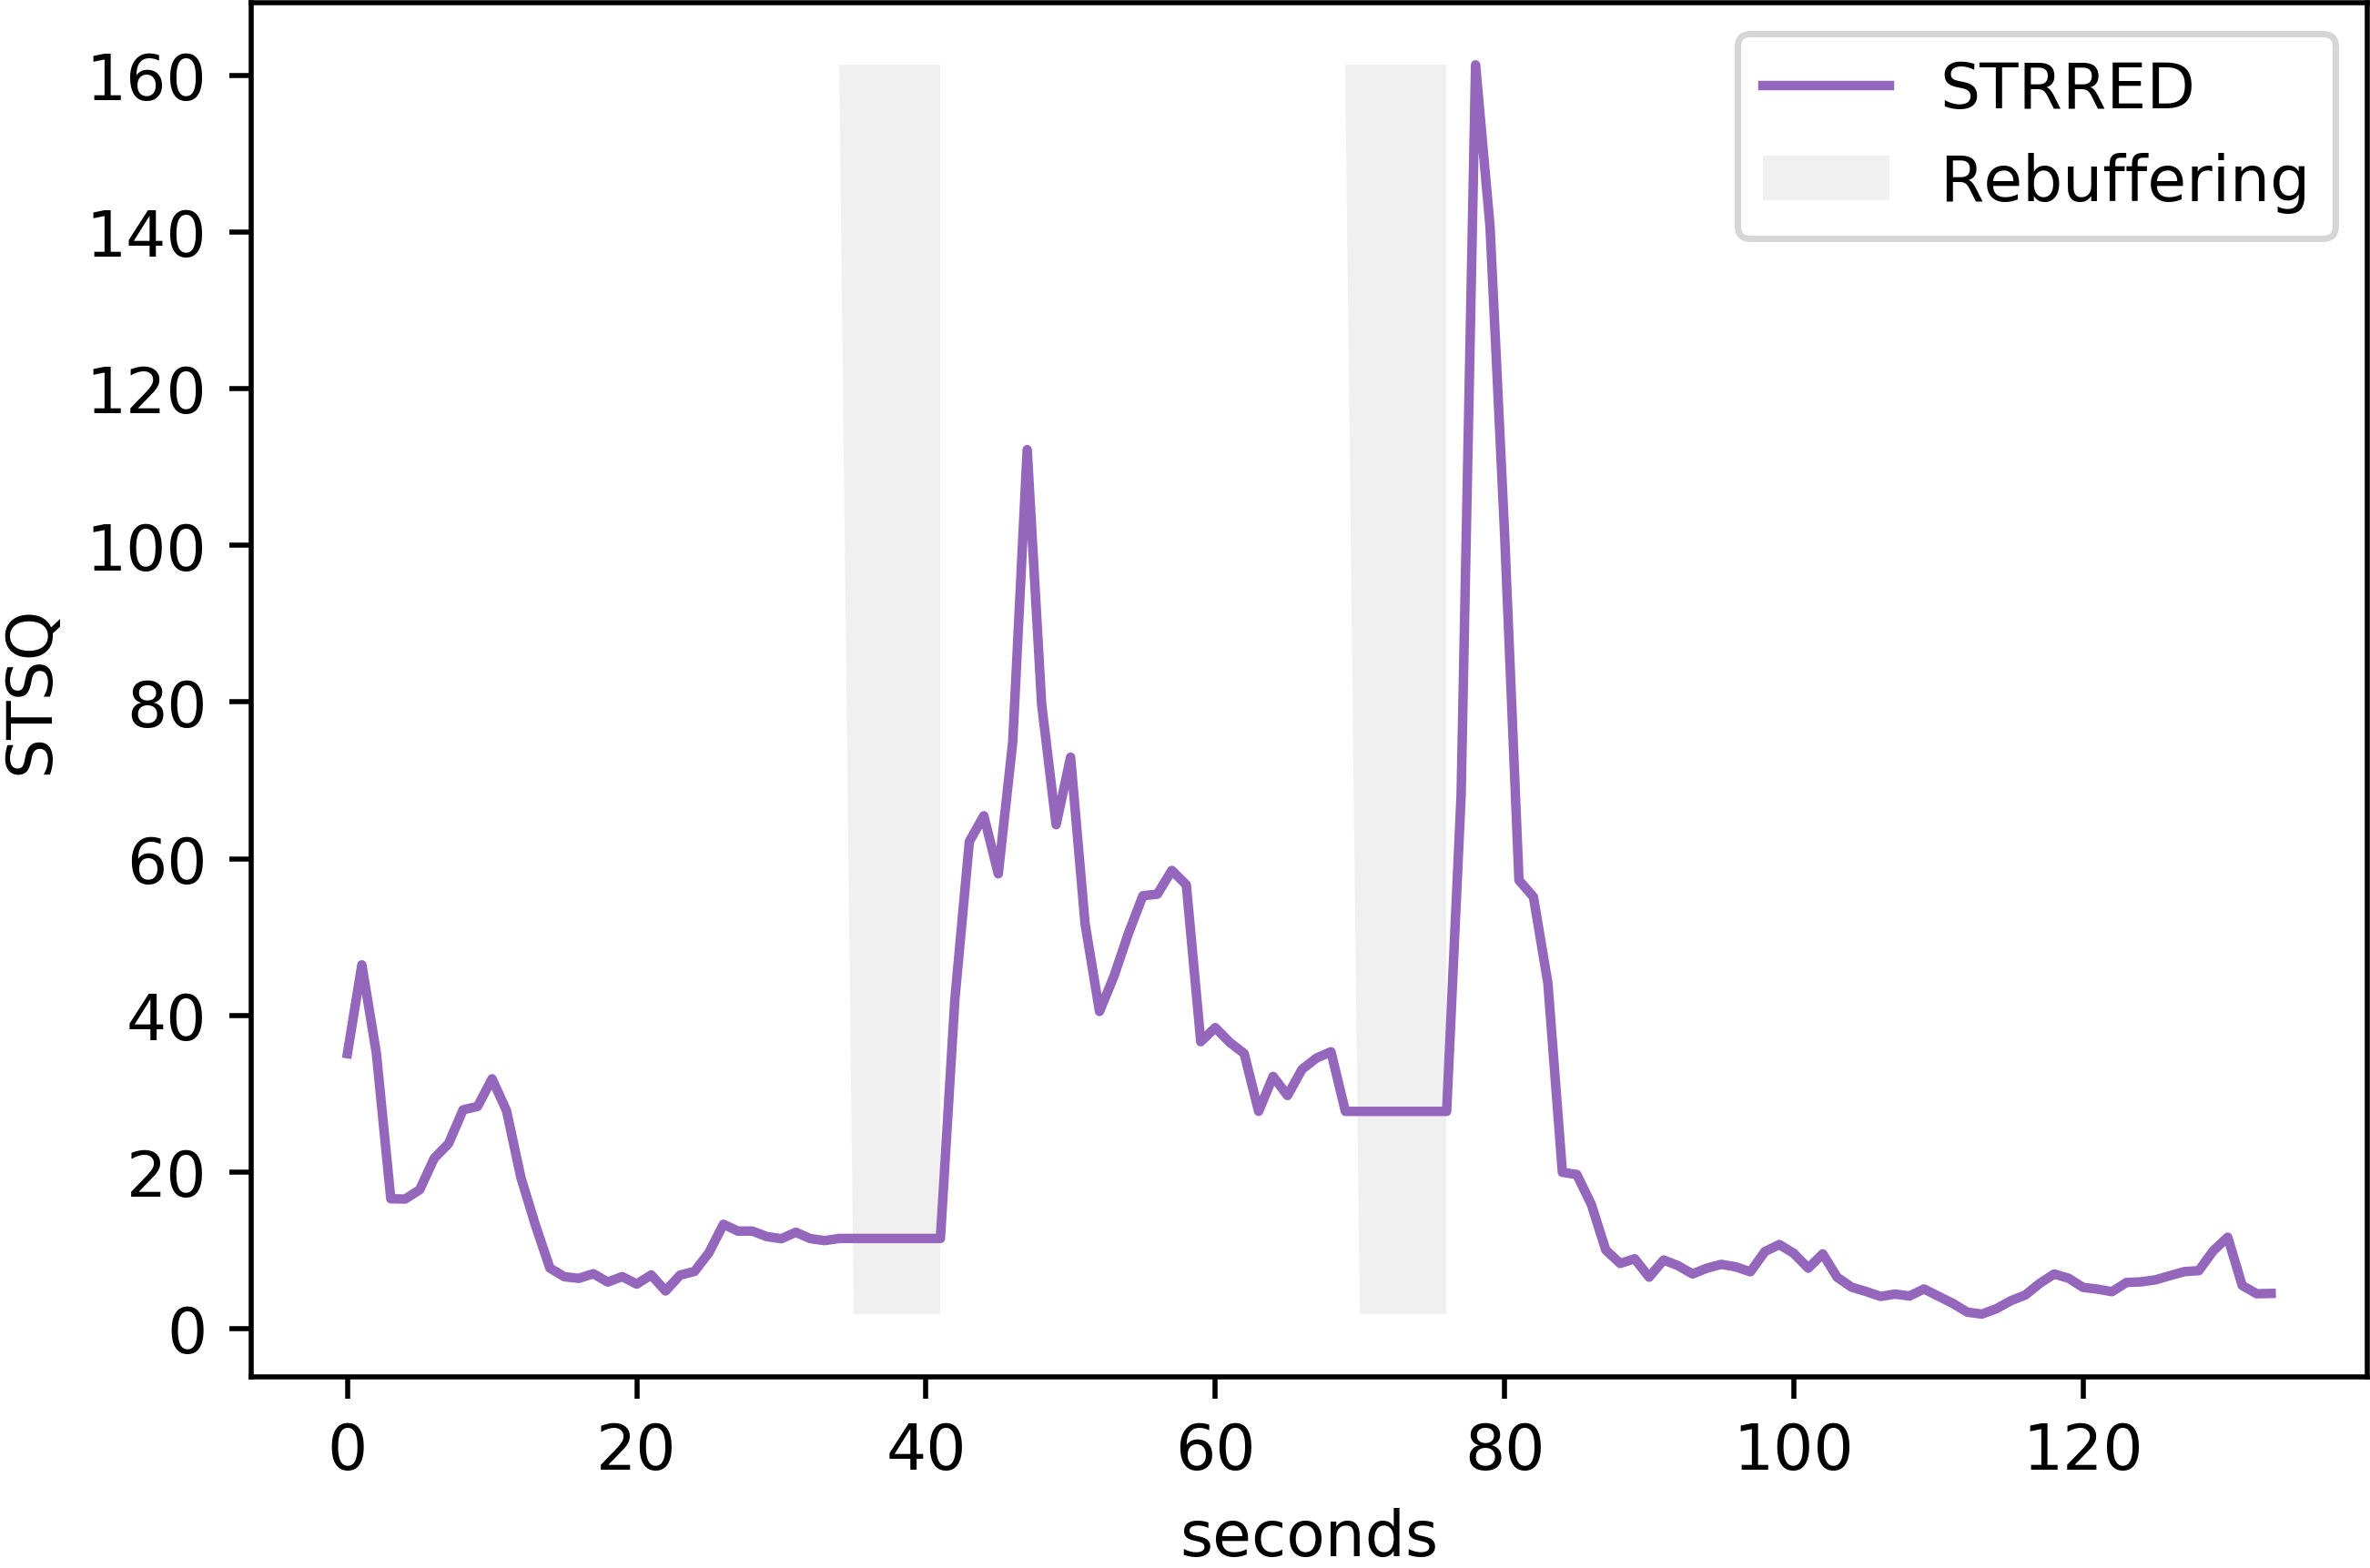
\includegraphics[width=\textwidth]{\FigsDir/features_STSQ.png}
    \caption{STSQ}
    \label{fig:InputFeatures_STSQ}
  \end{subfigure}
  \hfill
  \begin{subfigure}{0.48\linewidth}
    \centering
    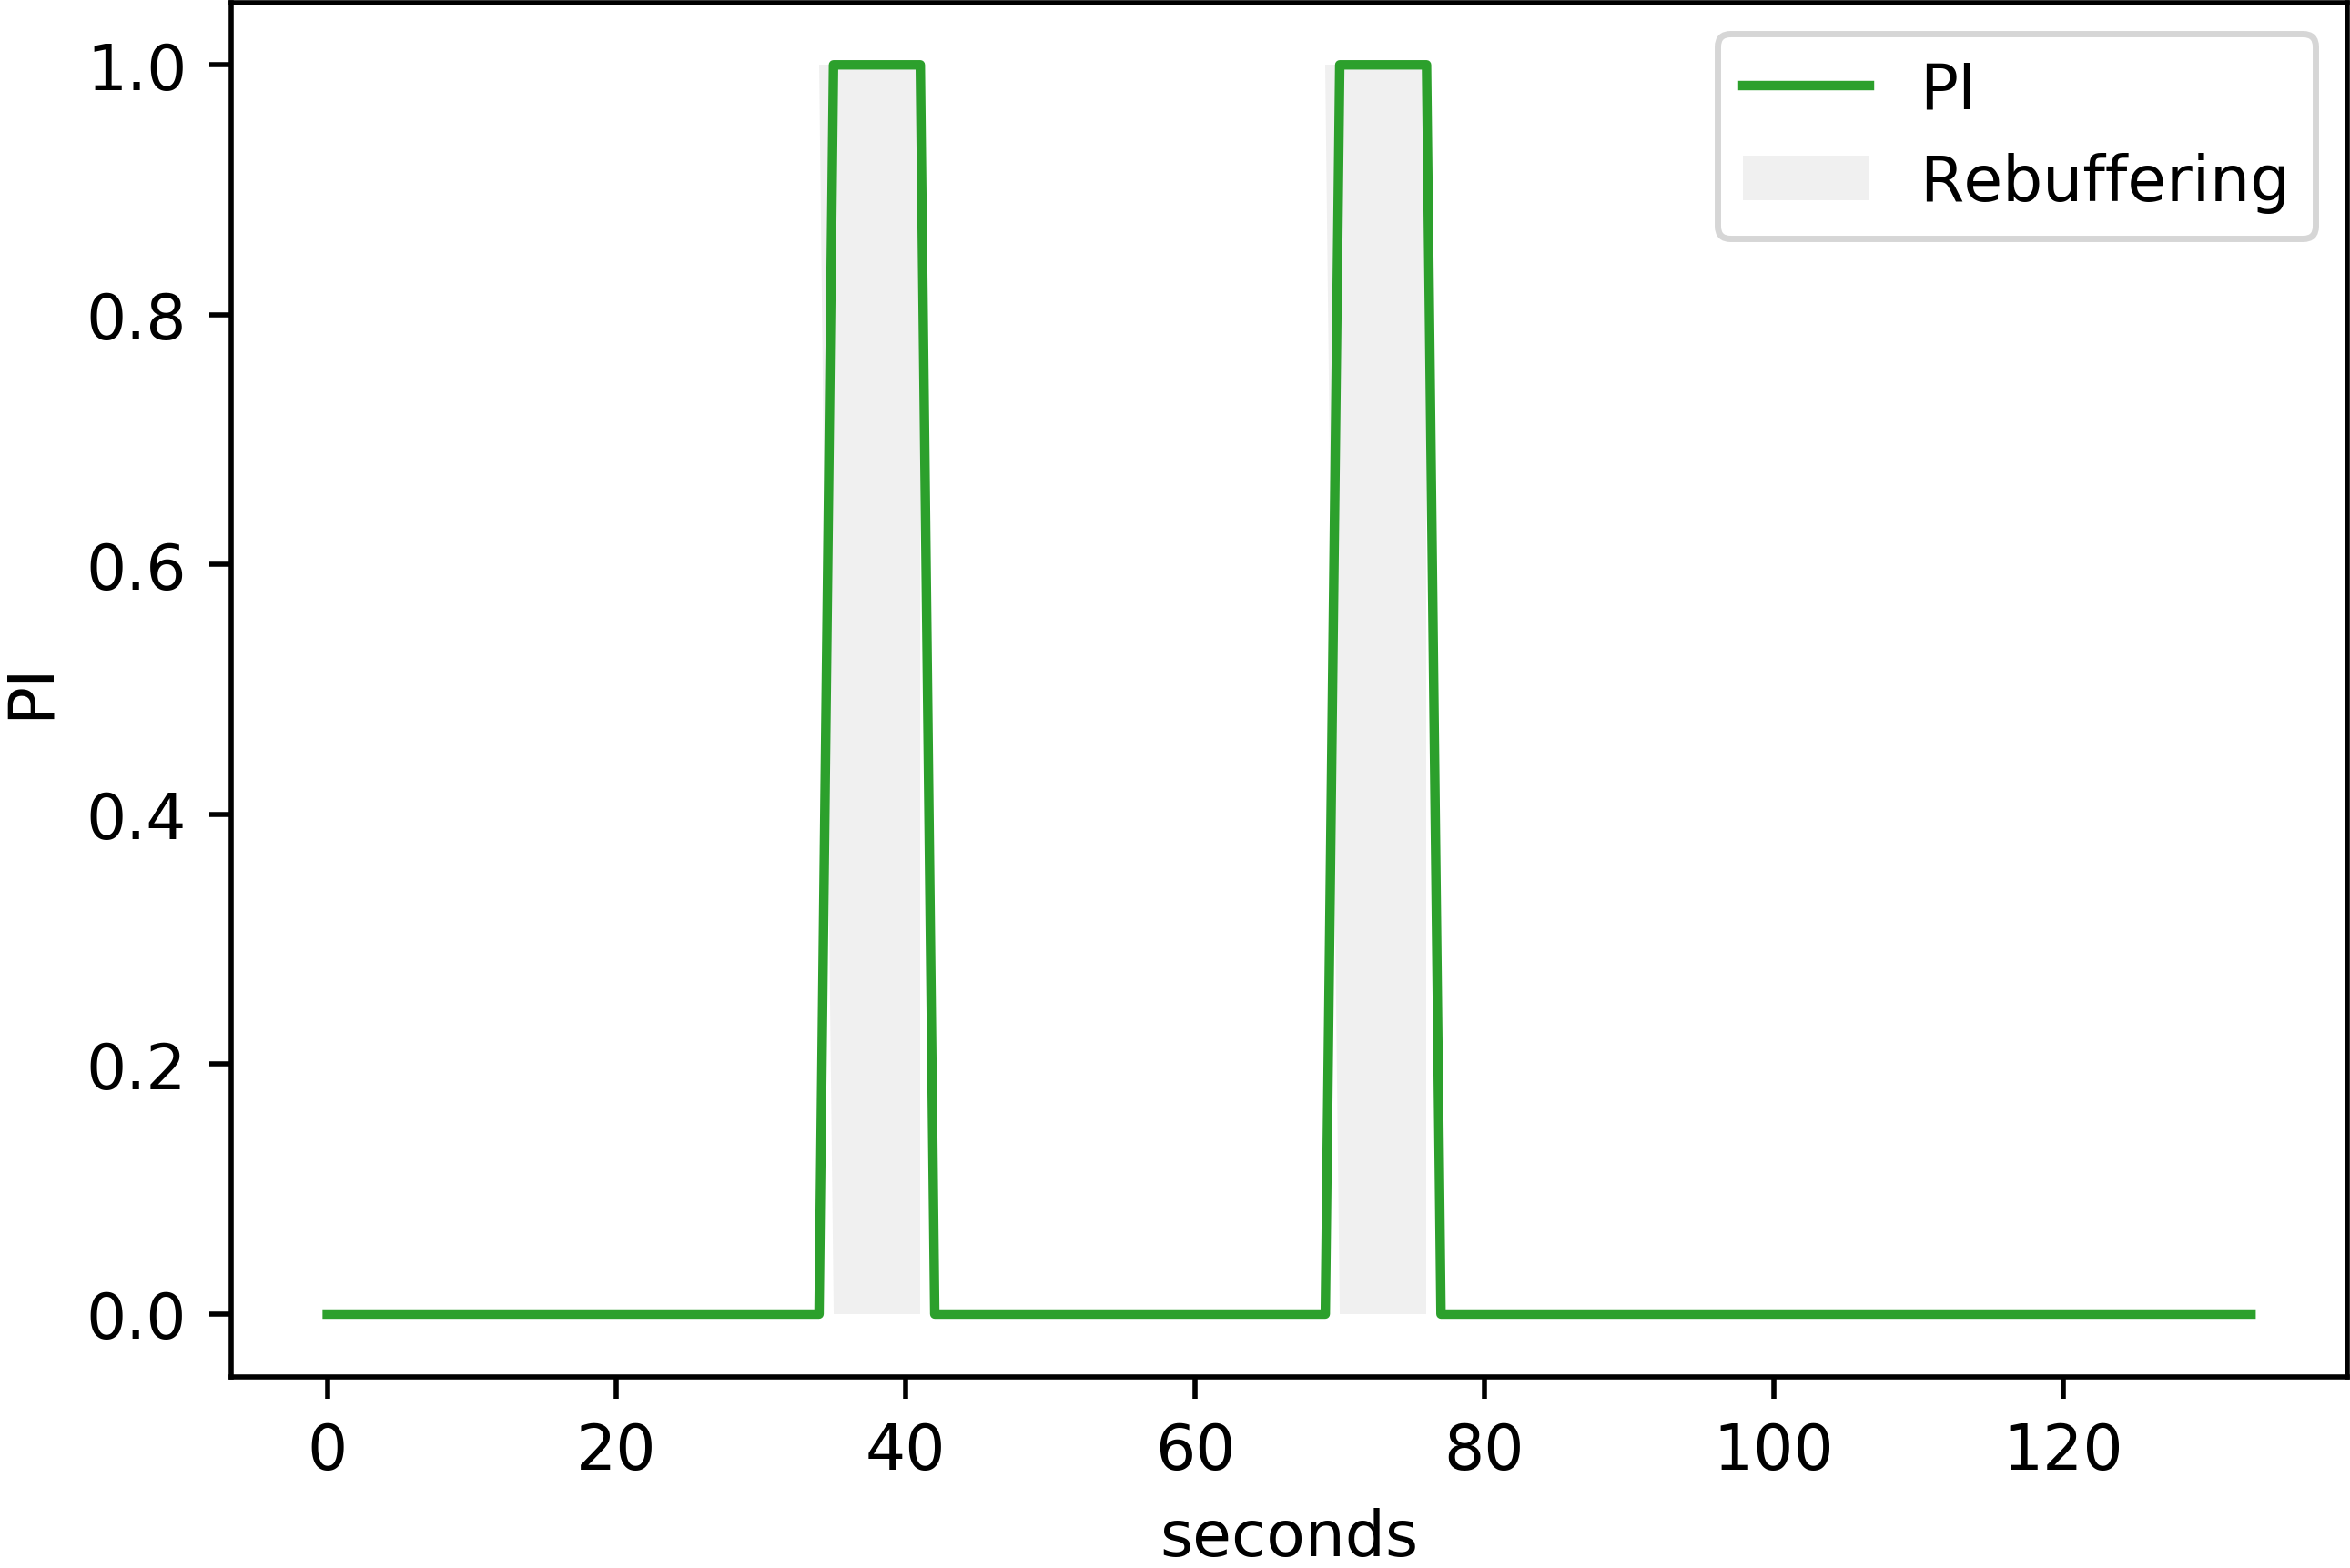
\includegraphics[width=\textwidth]{\FigsDir/features_PI.png}
    \caption{PI}
    \label{fig:InputFeatures_PI}
  \end{subfigure}
  
  \vspace{6pt}
  
  \begin{subfigure}{0.48\linewidth}
    \centering
    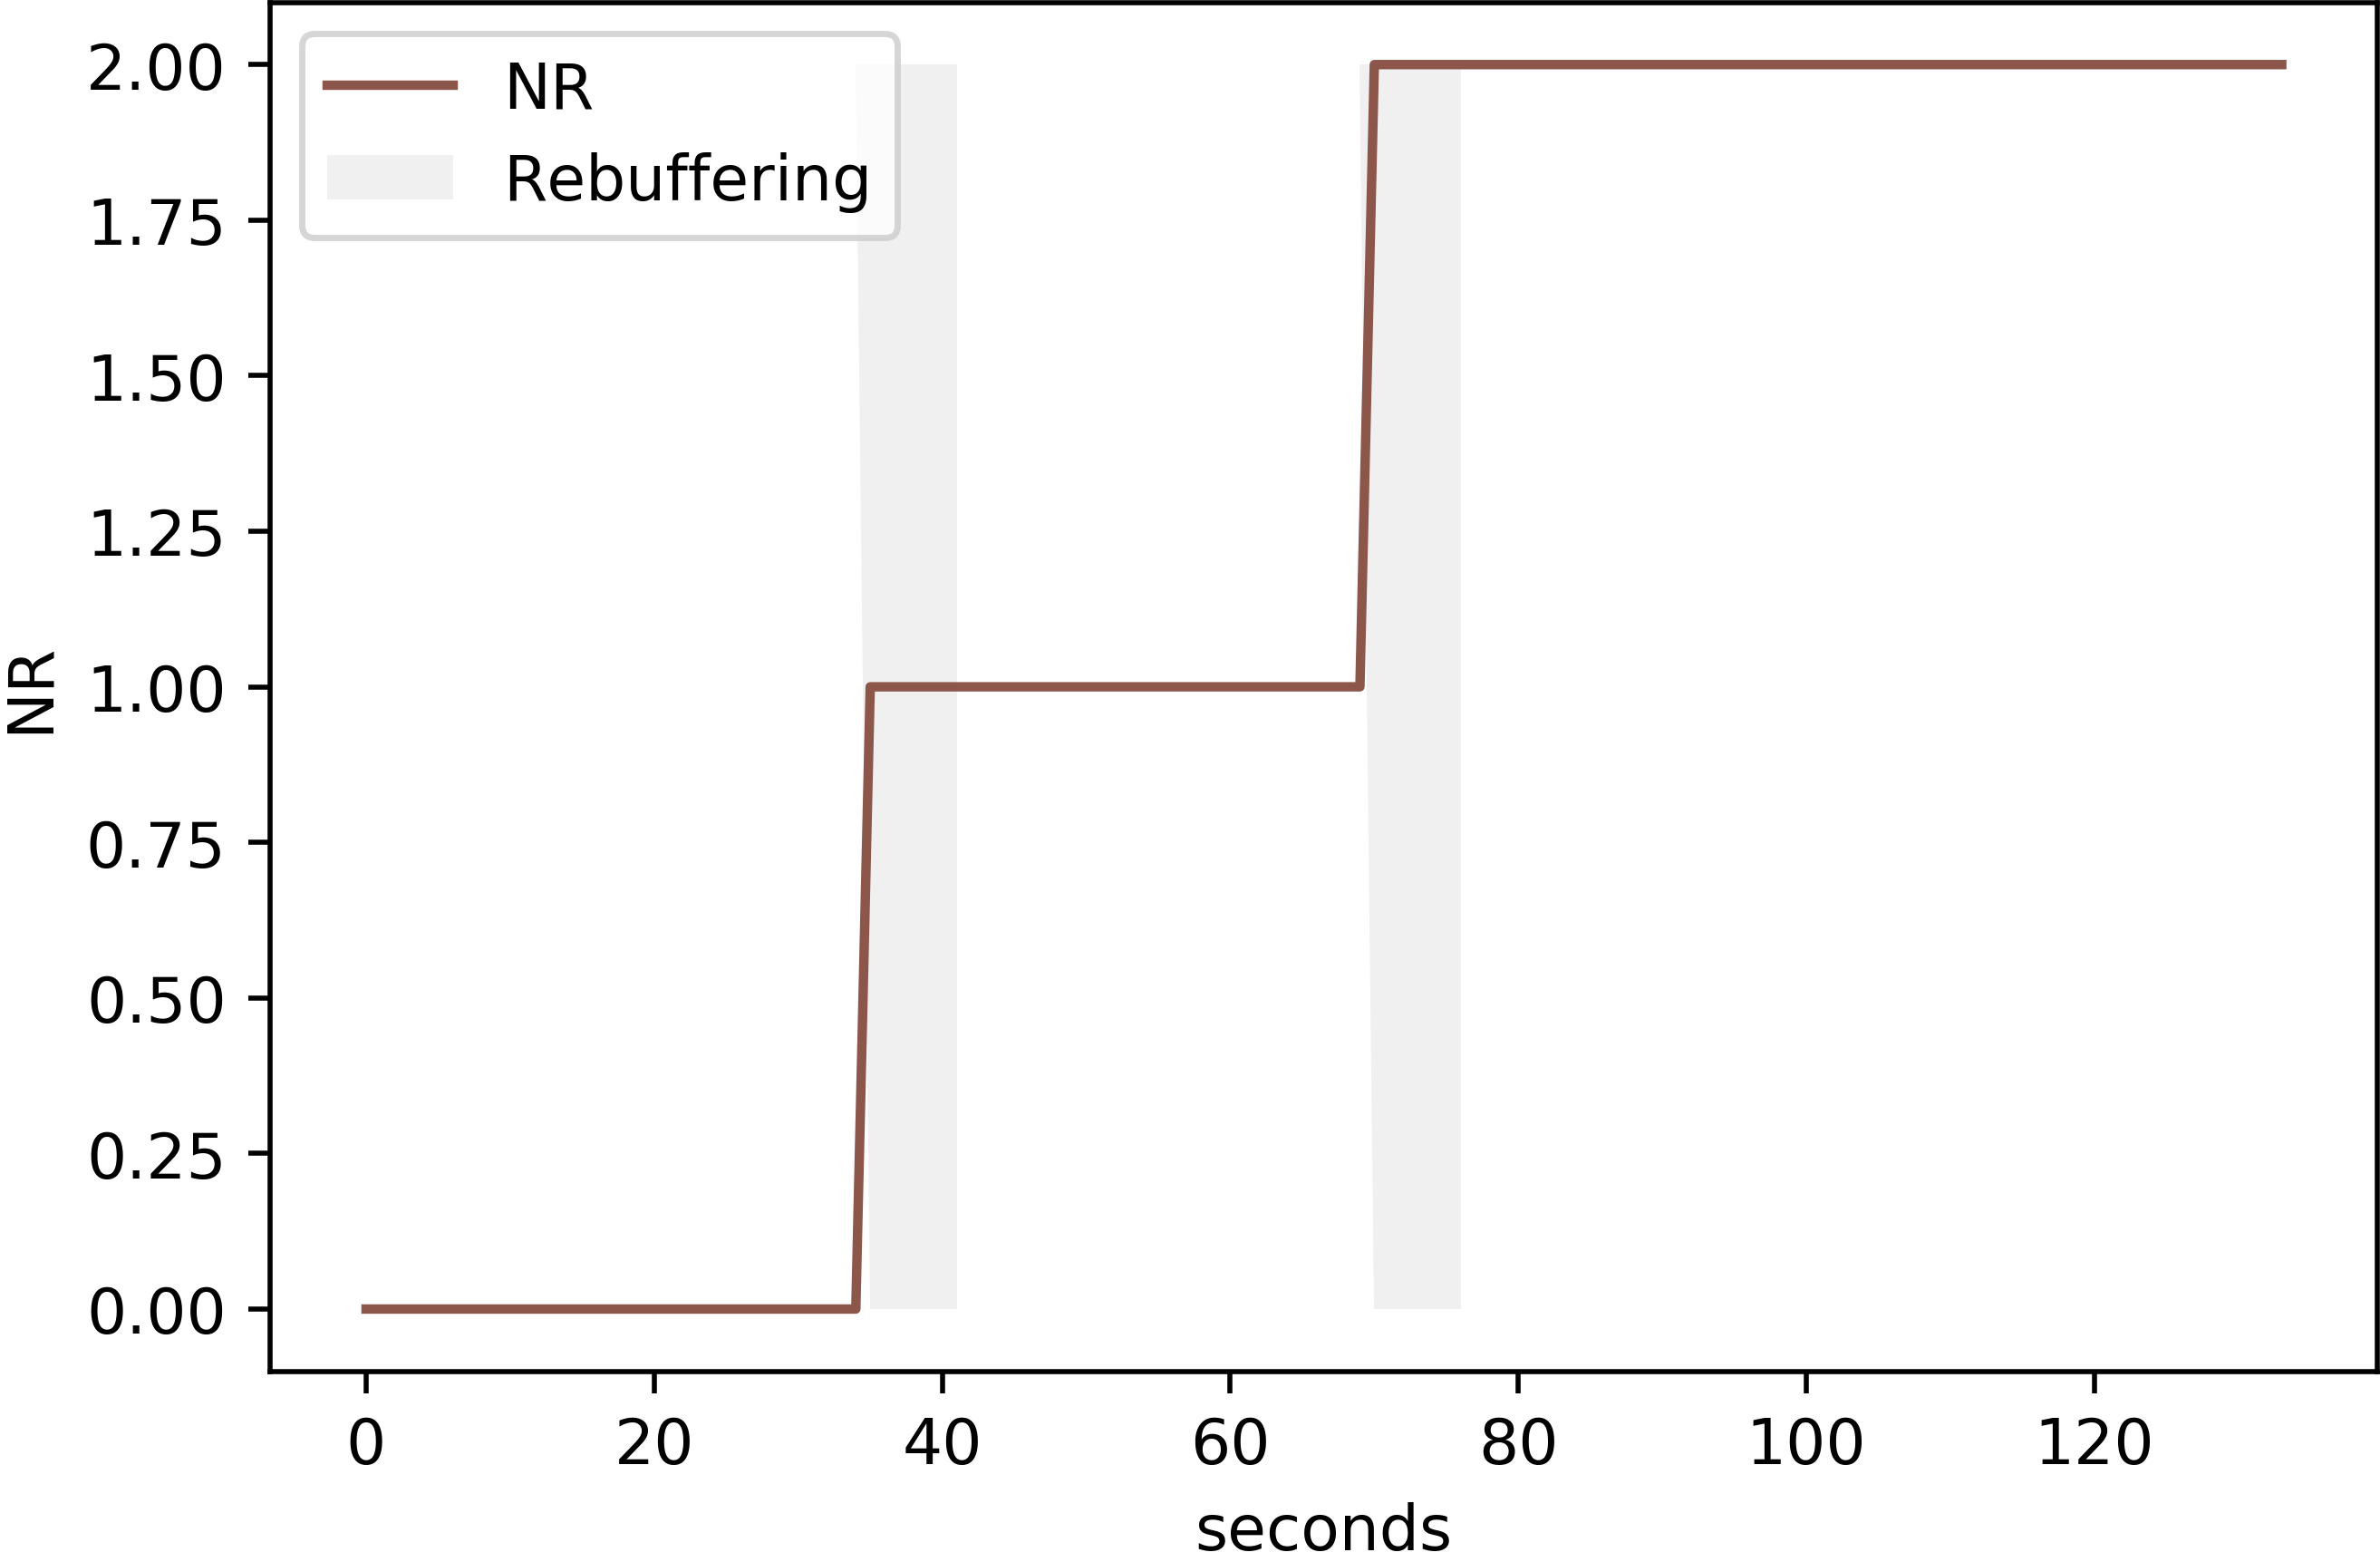
\includegraphics[width=\textwidth]{\FigsDir/features_NR.png}
    \caption{NR}
    \label{fig:InputFeatures_NR}
  \end{subfigure}
  \hfill
  \begin{subfigure}{0.48\linewidth}
    \centering
    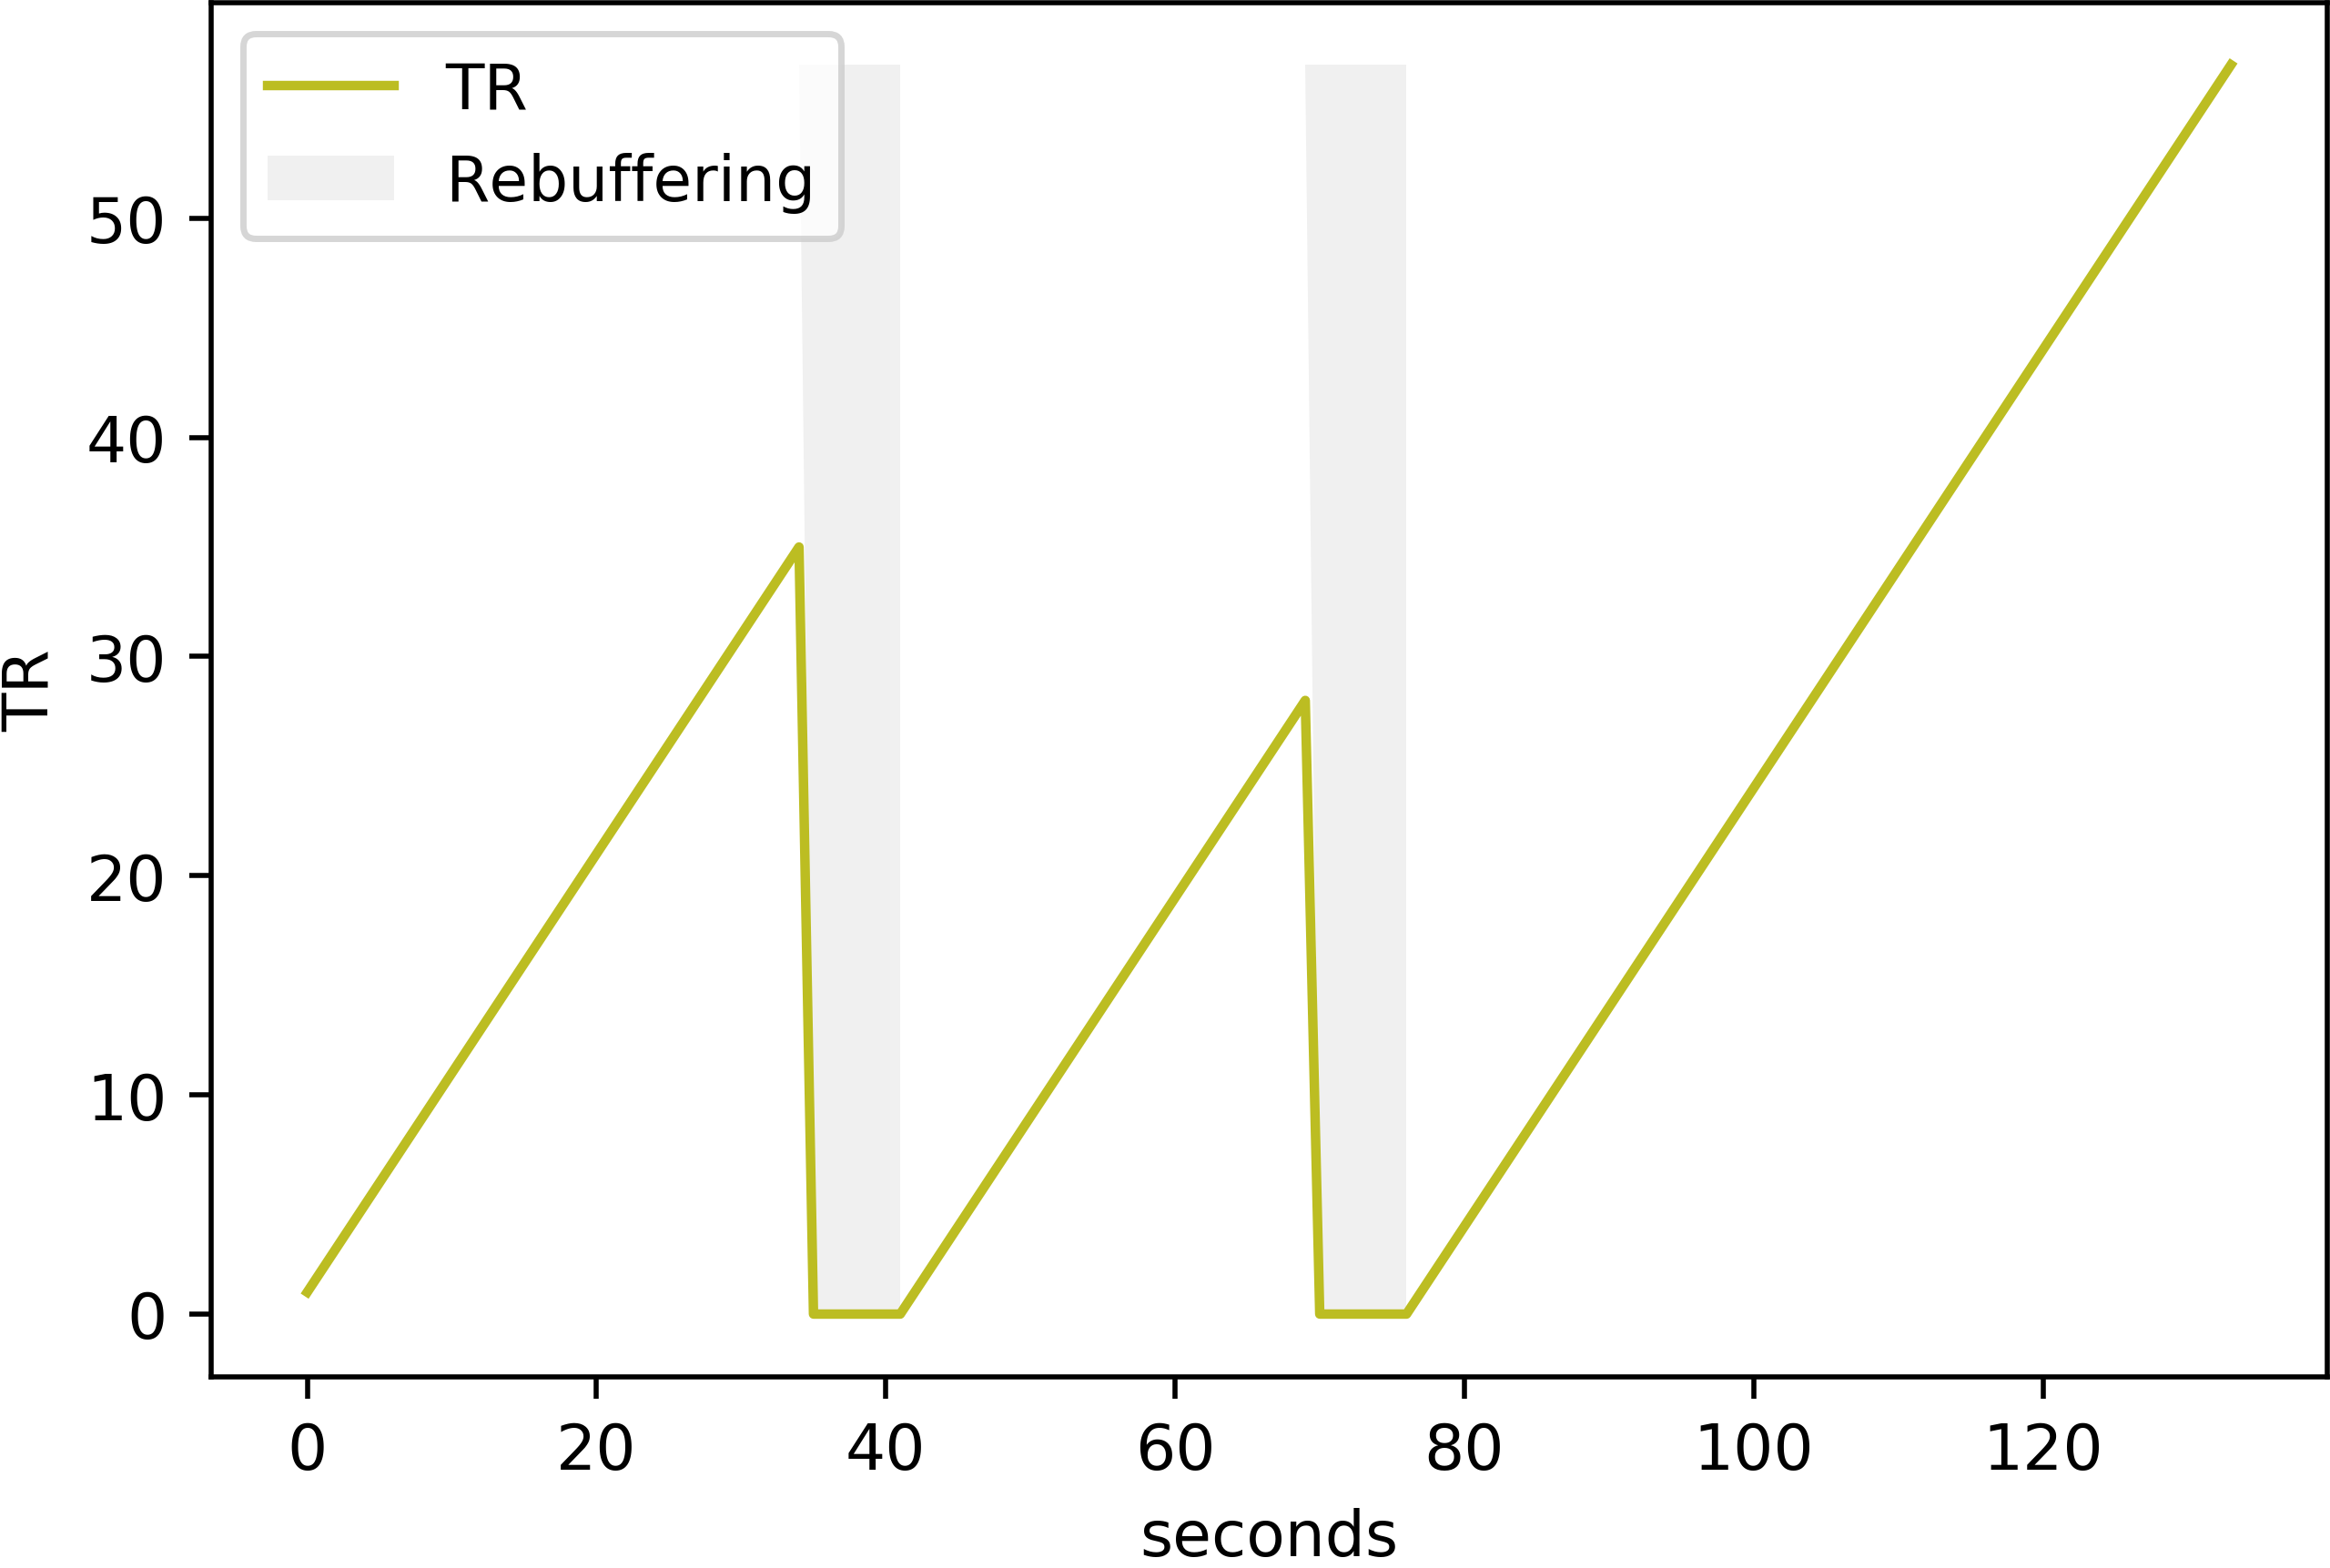
\includegraphics[width=\textwidth]{\FigsDir/features_TR.png}
    \caption{TR}
    \label{fig:InputFeatures_TR}
  \end{subfigure}
  
  \caption{Example of rebuffering and bitrate-related features represented by STSQ, PI, NR, and TR}
  \label{fig:InputFeatures}
\end{figure}


Video streaming users are sensitively affected by the video quality, known as \textit{short time subjective quality} (STSQ) \cite{QoEModel_TimeVaryingSubjectiveQuality}.
STSQ is defined as the visual quality of video being rendered to the user and can be predicted using any of the robust video quality assessment (VQA) metrics, such as Spatio-Temporal Reduced Reference Entropic Differences (STRRED) \cite{STRRED}, Multi-Scale Structural Similarity (MS-SSIM) \cite{MSSSIM}, Peak Signal to Noise Ratio (PSNR) \cite{PSNR}, etc.
Recent experiments have demonstrated that STRRED is a robust and high-performing VQA model when being tested on a very wide spectrum of video quality datasets, on multiple resolution and device types \cite{FeaturePredictionQoE, QoEModel_NLSS, QoEModel_LSTM}.
Therefore, STRRED is utilized to measure the STSQ.

Rebuffering greatly impacts the user's QoE \cite{StallingEvents}.
Thus, rebuffering information such as rebuffering length, rebuffering position and the number of rebuffering events must be investigated.
As a result, two rebuffering-related inputs are employed.
Firstly, \textit{playback indicator} (PI) \cite{QoEModel_NARX_DynamicNetworks, QoEModel_NLSS, QoEModel_LSTM} is defined as a binary continuous-time variable, specifying the current playback status, i.e., $1$ for rebuffering and $0$ for normal playback.
Secondly, as the user's annoyance increases whenever a rebuffering event occurs \cite{StallingEvents}, the \textit{number of rebuffering events} (NR) happened from the start to the current time instant of the session is considered.

Besides, the user's QoE is also affected by memory factors.
For example, more recent experiences have larger impacts on the user's perceived video quality, known as the recency effect \cite{Recency, NetflixQoE, LFOVIA}.
To capture the relation between the recency effect and the user's QoE, \textit{time elapsed since the last video impairment} (i.e., bitrate switch or rebuffering occurrence) \cite{QoEModel_NARX_DynamicNetworks, QoEModel_NLSS, QoEModel_LSTM}, denoted as TR, is utilized.


All the considered QoE influence factors are fed to the BiLSTM-QoE model to predict the instantaneous QoE. The examples of four factors (including STSQ, PI, NR, and TR) are illustrated in Figure \ref{fig:InputFeatures}.




\subsection{LIVE Netflix Video QoE Database}


The BiLSTM-QoE model is evaluated on the LIVE Netflix Video QoE Database \citep{NetflixQoE}.
The database consists of 112 distorted videos generated from 14 video contents by 8 different playout patterns
including bitrate changing, rebuffering events and mixtures of both \citep{NetflixQoE}.
The training and testing strategy are defined in \citep{QoEModel_LSTM}.
For each video $j$ in the database, one train-test set is created,
the model is trained on the set of videos that do not have the same content
and the playout pattern as the video $j$ in the test set.
Therefore, there are 112 train-test sets, each contains 1 testing videos and 91 training videos
(excludes 14 videos with the same content and 7 with the same playout pattern).
With this strategy, content and pattern dependencies are eliminated.




\subsection{Evaluation Results}


\Figure[tb][width=\linewidth]{\FigsDir/results.png}
  {QoE prediction performance of the BiLSTM-QoE over the LIVE Netflix Video QoE Database.\label{fig:BiLSTM_Accuracy}}
\Table[b]{\TablesDir/accuracy}
  {QoE prediction performance of the BiLSTM-QoE over the LIVE Netflix Video QoE Database.\label{tbl:BiLSTM_Accuracy}}


The BiLSTM-QoE model was trained and tested as described above.
The QoE prediction on the database using 4 features (i.e. STSQ, PI, TR and NR) are illustrated in Figure 6. 
The mean QoE prediction performance results are tabulated in Table \ref{tbl:BiLSTM_Accuracy},
also compared with other QoE models in the same database.
There are three considered evaluation criteria: Pearson Correlation Coefficient (PCC), Spearman Rank Correlation Coefficient (SROCC), and Root Mean Squared Error (RMSE).
The proposed model outperforms LSTM-QoE \citep{QoEModel_LSTM}, NLSS-QoE \citep{QoEModel_NLSS} and NARX \citep{QoEModel_NARX_DynamicNetworks} in terms of QoE prediction accuracy.
This is because the BiLSTM networks are very suitable to learn more useful information from time-varying features,
thereby allows this model to achieve the best performance among all the referenced models.

\section{Discussion}
\label{BiLSTM:sec:Discussion}
The results demonstrate that the proposed model using BiLSTM, measuring both forward and backward directions, is capable of learning more useful information from QoE influence factors such as video quality, bitrate switching, and rebuffering events.
For example, in pattern \#1 (which is ideal circumstances where no rebuffering or bitrate changes occurred), \#2 (one rebuffering occurred), \#6 (two rebufferings occurred close together), the QoE prediction performance is very good and the trends of the predicted QoE are pretty similar with the subjective QoE.
It has proved that the model can adapt well to different scenarios occurring during a streaming session.
However, the accuracy of the model may fluctuate across different playout patterns in the database.
For example, the accuracy on patterns without rebuffering (\#1, \#3, \#5, \#8) are relatively worse, due to the fact that among four features, only the STSQ values are nonzero, thereby, the prediction model depends only on STSQ inputs that may hurt the accuracy.
Thus, it is necessary to consider the other general valuable features whose values are nonzero in any scenarios, to achieve higher prediction accuracy.

\section{Summary}
\label{BiLSTM:sec:Summary}
In this chapter, the BiLSTM-QoE model was presented to improve the QoE prediction accuracy.
Unlike unidirectional LSTM only measuring forward direction, BiLSTM considers both forward and backward dependencies, thereby it has the ability to avoid filtering out the useful information.
Despite the various QoE influence factors and the complex interactions among them, the model can provide an accurate prediction user’s QoE.


In the next chapter, the CNN-QoE model is introduced to further improve the QoE prediction accuracy.
Furthermore, the model also focus on minimizing the computational complexity, resulting in a QoE prediction model that can be utilized in real-time QoE modeling and continuous monitoring.

\chapter{CNN-QoE Model}
\label{ch:CNN}


\renewcommand{\SectionsDir}{Chapter4/Sections}
\renewcommand{\FigsDir}{Chapter4/Figs}
\renewcommand{\TablesDir}{Chapter4/Tables}


\section{Introduction}
\label{CNN:sec:Introduction}
Most of existing works only focused on modeling the overall or the instantaneous QoE, which have shown insufficient characteristics.
The overall QoE \cite{QoEModel_OP_EstimatingQoE, QoEModel_OP_DerivingValidatingUserExperience, QoEModel_OP_VideoQualityMetric}, which demonstrates the final subjective judgment for a streaming session, can only be assessed when the viewer finishes watching.
Therefore, the overall QoE cannot be applied for real-time QoE monitor and also does not give sufficient information about events occurring during the session.
Although the instantaneous QoE \cite{QoEModel_TimeVaryingSubjectiveQuality, QoeModel_ShortLongTermQualityModel}, on the other hand, can provide the instant perceived video quality at a certain moment, it only reflects locally the quality assessment within a specific time range, without considering the cumulative effects of prior events.
Hence, it is highly sensitive to video impairments due to hysteresis effect \cite{TemporalHysteresisModel, StallingEvents} and does not precisely express the user's perceived video quality.
In contrast, modeling and predicting the user's cumulative perception to a streaming video content are able to provide lots of advantages for QoE monitor and control systems since it not only reflects the user's overall satisfaction but also reveals the impact of distorted events happening during the streaming session.



In addition, according to \citep{QoEDef_Qualinet}, QoE is defined as the results from the fulfillment of the user's expectation to the enjoyment of the application or service based on his or her \textit{personality} and \textit{current state}.
Here, "personality" defines "the characteristics of a person that account for consistent patterns of feeling, thinking and behaving", whereas, "current state" stands for "situational or temporal changes in the feeling, thinking or behavior of a person".
Therefore, human-related influence factors (e.g., perceptual factors, memory effect, user's interest in video content) play a crucial role in accurately modeling the user's QoE.


Some studies investigate and quantify the impact of perceptual factors \cite{QoEModel_OP_EstimatingQoE, QoEModel_OP_DerivingValidatingUserExperience, QoEModel_OP_VideoQualityMetric, QoEModel_TimeVaryingSubjectiveQuality, QoeModel_ShortLongTermQualityModel}.
However, the authors usually abandon the temporal dynamics and historical experience of the user's satisfaction, which are referred to as the memory effects \cite{MemoryEffects_WebQoE}.
Some other studies attempt to clarify the role of primacy and recency effects \cite{QoEModel_BitrateDistribution, QoEModel_OM_DistortionsRebuffMemory, QoEModel_NARX_DynamicNetworks, LFOVIA, QoEModel_TVQoE_ContinuousTimeQoE, QoEModel_NLSS, QoEModel_LSTM}, resulting in the high accurate QoE prediction.
Typically, the primacy and recency effects \cite{PrimacyVsRecency} determine the memory influence of impairments occurring at the beginning and the end of streaming session \cite{NetflixQoE}, respectively.
Besides, the effect of unpleasant events which take place in the middle of the session also leaves a considerable impact on the perceived video quality \cite{NetflixQoE,StallingEvents}.
Theoretically, such impacts can be represented by an exponential deterioration of memory retention in time (defined by \textit{forgetting curve}) \cite{UserForgetful, EvaluatingForgettingCurves, Ebbinghaus_ForgettingCurve} for infrequent events or by \textit{repetition} \cite{StallingEvents, Ebbinghaus_ForgettingCurve} for the repeated impairments.
However, the influence of forgetting behavior and repetition has not been carefully investigated in existing QoE models.
Therefore, to fully express human memory effects on QoE assessment, in addition to the primacy and recency effects, the forgetting curve and repetition should be involved in the discussion.


Apart from that, the factors that relate to video content also have a noticeable effect on perceived QoE. Those factors might be type of video, video complexity \cite{EffectSizesOfInfluenceFactors}, etc.
Additionally, some studies (e.g., \cite{QoSImpactUserVideoClips, SubjectiveQualityPairedComparison, QoEEvaluation_IPTV_Services}) have found that the user's interest in video content possibly generates the bias in his/her QoE evaluation.
More concretely, the user tends to provide higher QoE scores for more attractive video contents.
Such a behavior is influenced by the so-called degree of interest (DoI) which clarifies the interestingness of different video content, or the ability of the video content to attract the user and keep the user's interest \cite{VisualContent}.
However, existing studies often neglect this factor due to the fact that these numerical values might vary upon different users based on their personal interests.


For those reasons, in this chapter, we present a cumulative QoE model that extremely well quantifies multiple effects of human-related factors, that is to say, perceptual influence factors, memory effect and degree of interest (DoI).
In order to assess the accuracy in predicting cumulative QoE, the cumulative QoE model is evaluated over LFOVIA database \cite{LFOVIA} and through the subjective evaluation.
Evaluation results demonstrate that the cumulative QoE at different moments within a streaming session is precisely predicted by the model.
It shows the potential of cumulative QoE that can be utilized as a better alternative than either overall QoE or instantaneous QoE in QoE monitoring and management.

The rest of this chapter is organized as follows.
Section \ref{Cumulative:sec:Proposals} investigates the influence of human-related factors and presents the cumulative QoE prediction model.
 Section \ref{Cumulative:sec:Evaluation} evaluates the performance of the proposal and discusses the advantages and disadvantages.
 Section \ref{Cumulative:sec:Summary} summarizes this chapter.

\section{Temporal Convolutional Network}
\label{CNN:sec:TCN}
\Figure[tb][width=0.7\linewidth]{\FigsDir/tho1.png}
   {An illustration of a stack of causal convolution layers with the convolution filter size of $1 \times 2$.\label{fig:CausalConv}}

\Figure[tb][width=0.7\linewidth]{\FigsDir/tho2.png}
   {An illustration of a stack of dilated causal convolution layers with the convolution filter size of $1 \times 2$.\label{fig:DilatedConv}}
   
\Figure[tb][width=0.6\linewidth]{\FigsDir/tho3.png}
   {The residual block in TCN architecture.\label{fig:TCN_residualBlock}}

In this section, TCN architecture is briefly discussed to summarize its advantages and disadvantages in sequence modeling tasks. Thereby, the conclusions of this section will be the crucial foundation for the subsequent improvements proposed in CNN-QoE, which are stated in Section \ref{CNN:sec:Proposals}.

%=========================================

\subsection{1D Convolutions}

CNN was traditionally designed to operate on two dimensions (2D) data such as images.
An input image is passed through a series of 2D convolution layers.
Each 2D convolution applies and slides a number of 2D filters through the image.
To adapt CNN for time-series data, TCN utilizes 1D convolution where the filters exhibit only one dimension (time) instead of two dimensions (width and height).
Concretely, a time-series input is convolved with a filter size of $1 \times k$.

Furthermore, 1D convolutions are well-suited for real-time tasks due to their low computational requirements.
1D convolutions require simple array operations rather than matrix operations, hence, the computational complexity is significantly reduced in comparison with 2D convolutions.
In addition, the convolution operations allow fully parallel processing, resulting in a significant improvement of computational speed.


%=========================================

\subsection{Causal Convolutions}

A \textit{causal convolution} is a convolution layer to ensure there is no information "leakage" from future into past.
In other words, given an time-series input $x_0,..., x_{T}$, the predicted output $\widehat{y}_t$ at a time instant $t$ depends only on the inputs at time $t$ and earlier $\mathbf{x}_t, \mathbf{x}_{t-1}, ...,\mathbf{x}_{t-r+1}$.
For instance, as illustrated in Figure \ref{fig:CausalConv}, the predicted $\widehat{y}_8$ is computed by a combination of the inputs $x_1, ..., x_8$.
It can be observed that, in order to achieve a long effective history size or a large receptive field size, an extremely deep network or very large filters are needed, which significantly increases the model computational complexity.
Thus, TCN architecture utilizes dilated causal convolutions rather than causal convolutions.
The advantages and disadvantages of dilated causal convolutions are discussed below.

%=========================================

\subsection{Dilated Causal Convolutions}

TCN adopts a dilated causal convolution comprising of the causal and the dilated convolutions.
The causal convolution has already been described in the previous subsection.
Meanwhile, dilated convolution \cite{Network_Dilated1, Network_Dilated2, Network_Dilated3} is a convolution where the convolution filter is applied to a larger area than its length by skipping input values with several steps.
Therefore, the dilated causal convolution can effectively allow the network to operate on a larger scale than the one with a normal convolution while ensuring that there is no leakage of information from the future to the past.
The dilated causal convolution is defined as:

\begin{equation}
  D(t) = \sum_{i=0}^{k-1} f(i) \cdot \mathbf{x}_{t-d \cdot i}
  \label{eqn:TCN_dilatedConv}
\end{equation}
where, $d$ is the dilation factor, $f$ is a filter size of $1 \times k$.
$d$ exponentially increases with the depth of the network (i.e., $d = 2^l$ at layer $l$ of the network).
For instance, given the network with $L$ layers of dilated causal convolutions $l = 1, ..., L$, the dilation factors exponentially increase by a factor of $2$ for every layer:

\begin{equation}
  d \in [2^0, 2^1, ..., 2^{L-1}]
  \label{eqn:TCN_dilatedFactor}
\end{equation}

Figure \ref{fig:DilatedConv} depicts a network with three dilated causal convolutions for dilations 1, 2, and 4.
Using the dilated causal convolutions, the model is able to efficiently learn the connections between far-away time-steps in the time series data.
Moreover, as opposed to causal convolutions in Figure \ref{fig:CausalConv}, the dilated causal convolutions require fewer layers even though the receptive field size is the same.
A stack of dilated causal convolutions enables the network to have a very large receptive field with just a few layers, while preserving the computational efficiency.
Therefore, dilated causal convolutions reduce the total number of learnable parameters, resulting in more efficient training and light-weight model.

However, the dilated causal convolutions have problem with local feature extraction.
As shown in Figure \ref{fig:DilatedConv}, it can be seen that the filter applied to the time-series input is not overlapped due to the skipping steps of the dilation factor.
As long as the dilation factor increases, the feature is extracted from only far-apart time-steps, but not from adjacent time-steps.
Therefore, the local connection among adjacent time-steps is not fully extracted at higher layers.

%=========================================

\subsection{Residual Block}

The depth of the model is important for learning robust representations, but also comes with a challenge of vanishing gradients.
The residual block has been found to be an effective way to address this issue and build very deep networks \cite{Network_Residual1}.
A residual block contains a series of transformation functions $\emph{F}$, whose outputs are added to the input $\mathbf{x}$ of the block:

\begin{equation}
  o = Activation(x+\emph{F}(x))
\end{equation}

The residual block is used between each layer in TCN to speed up convergence and enable the training of much deeper models.
The residual block for TCN is shown in Figure \ref{fig:TCN_residualBlock}.
It consists of dilated causal convolution, ReLU activation function \cite{Network_Relu}, weight normalization \cite{Network_WeightNorm1}, and spatial dropout \cite{Network_Dropout1} for regularization.
Having two layers of dilated causal convolution in the TCN's residual block is suitable for complex challenges such as speech enhancement \cite{Network_TCN}.
Compared with speech signal data, sequential QoE data is much simpler.
That is to say, the two layers of dilated causal convolution are redundant and are not optimal for the QoE prediction problem.

% The $1 \times 1$ convolution is used to get the channels, which makes the addition of inputs and outputs compatible.

%=========================================

In TCN architecture, equations (\ref{eqn:TCN_dilatedConv}) and (\ref{eqn:TCN_dilatedFactor}) suggest that the TCN model heavily depends on the network depth $L$ and the filter size $k$.


\section{Model Architecture}
\label{CNN:sec:Proposals}
In this section, the model CNN-QoE is introduced to leverage the advantages and handles the problems of the TCN architecture \cite{Network_TCN} in QoE prediction for video streaming services.
The architecture employed for the CNN-QoE model is discussed in detail in the following subsections.
The model architecture hyperparameters are then analyzed to find the optimal values which can improve the QoE prediction accuracy, while minimizing the computational complexity.


\subsection{Proposed Model Architecture}
\label{sec:ProposedModel_Architecture}
\Figure[!t][width=0.95\linewidth]{\FigsDir/tho4.png}
   {The proposed CNN-QoE architecture.\label{fig:ProposedArchitecture}}
   
\Figure[!t][width=0.95\linewidth]{\FigsDir/tho5.png}
   {The proposed residual block used in the proposed architecture.\label{fig:ProposedResidualBlock}}
   
Figure \ref{fig:ProposedArchitecture} illustrates the overview of the CNN-QoE's architecture.
The CNN-QoE leverages the advantages of 1D convolutions, dilated causal convolutions and residual block in TCN architecture.
To adapt the TCN to QoE prediction tasks, a number of improvements are made as follows:

\begin{itemize}
  \item An initial causal convolution layer is added to the input and then connects to residual block which includes a dilated causal convolution layer.
  \item The residual block is simplified by leveraging the advantages of Scaled Exponential Linear Units (SeLU) activation function \cite{SeLU}.
\end{itemize}
These distinguishing characteristics are discussed as below.

%=========================================

\subsubsection{Causal convolution to extract local features}

The architecture of the proposed model comprises of one causal convolution layer and a stack of dilated causal convolutions, while the TCN consists of only a number of dilated causal convolutions.
A causal convolution layer is added between the input time-series and the first residual block as shown in Figure \ref{fig:ProposedArchitecture}.
This causal convolution layer can extract the local features of the adjacent time-steps in the sequential QoE data.
Afterward, the following dilated causal convolution layers are leveraged to extract the global features between far-apart time steps.
These layers help the model to learn the most informative features in the time series input, resulting in higher accuracy.

%=========================================

\subsubsection{SeLU activation function}

Activation function plays an important role in allowing the model to learn non-linear representations of the input features.
When training a deep learning model, the vanishing and exploding gradient are the most challenging problems that prevent the network from learning the optimal solution.
The TCN model gets rid of these problems by integrating
%==================================================================================
% \revise{
ReLU activation function \cite{Network_Relu},
% <explaination is not enough, only explained with the reference number in section III-4>
% }
%==================================================================================
weight normalization \cite{Network_WeightNorm1} and dropout \cite{Network_Dropout1} layer as shown in Figure \ref{fig:TCN_residualBlock}.
In the proposed CNN-QoE, those layers are replaced with the SeLU to leverage its advantages and simplify the residual block as shown in Figure \ref{fig:ProposedResidualBlock}.
SeLU is a self-normalizing activation function.
It converges to zero mean and unit variance when propagated through multiple layers during network training, thereby making it unaffected by vanishing and exploding gradient problems.
Moreover, SeLU also solves the "dying ReLU" problem where the ReLU function always outputs the same value of 0 for any input, so the gradient descent is not able to alter the learnable parameters.
At the same time, SeLU also reduces the training time and learns robust features more efficiently than other networks with normalization techniques, such as weight normalization \cite{SeLU}.
SeLU activation function described as follow \cite{SeLU}:

\begin{equation}
\label{eq:SeLU}
  SeLU(x) = \lambda \begin{pmatrix}
    x, & \textit{if } x > 0 \\ 
    \alpha \textit{exp}(x) - \alpha, & \textit{if } x \leq 0 
  \end{pmatrix}
\end{equation}

% which has the gradient:

% \begin{equation}
%   \frac{d}{dx}SeLU(x) = \begin{pmatrix}
%     \lambda & \textit{if } x > 0 \\
%     SeLU(x) + \lambda \alpha & \textif{if } x \leq 0
%   \end{pmatrix}
% \end{equation}
where $\alpha = 1.67733$ and $\lambda = 1.0507$. These are the same values as the ones proposed in \cite{SeLU}.

% \revise{(The reason why you use Scale Exponential Linear Units function here must be explained. Why not others?)}



\subsection{Architecture Hyperparameters Selection}
\label{sec:ProposedModel_Parameters}
\begin{table}[t]
  \caption{Hyperparameters for the best performance model.}
  \label{tbl:ModelHyperparameters}
  \centering
  \input{\TablesDir/tho.t1}
\end{table}

When training the model, an adequate set of architecture hyperparameters must be selected to achieve the best performance.
The proposed model consists of $L$ residual block layers, each layer contains a dilated causal convolution with a filter size of $1 \times k$, as shown in Figure \ref{fig:ProposedArchitecture} and \ref{fig:ProposedResidualBlock}.
Each dilated convolution layer has a dilation factor $d$ doubled at each layer up, as shown in (\ref{eqn:TCN_dilatedFactor}).
The proposed model depends on the network depth $L$ and the filter size $k$.
These hyperparameters control the trade-off between QoE prediction accuracy and computational complexity of the model.
To effectively optimize the hyperparameters, it is important to set a boundary for the space of possible hyperparameter values.

The user's QoE is mostly affected by the recent experiences, also known as the recency effect \cite{Recency, NetflixQoE, LFOVIA}.
The recency effect gradually decreases within 15 to 20 seconds \cite{NetflixQoE, LFOVIA} after distorted events (e.g., bitrate fluctuations, rebuffering events).
Therefore, the effective history or the receptive field size $r$ of the model cannot be larger than 20 time-steps

\begin{equation}
  r \leq 20
  \label{eqn:TCN_receptiveField_limit}
\end{equation}

Moreover, the receptive field depends on the number of dilated causal convolution layers $L$ and the filter size $k$.
For example, with $l \in [1, L]$, the receptive field $r$ can be determined by (\ref{eqn:TCN_receptiveField_2}) \cite{Network_Wavenet, Network_TCN}

\begin{equation}
 r = 2^{L} \mathrm{, if} \quad k = 2
 \label{eqn:TCN_receptiveField_2}
\end{equation}

or (\ref{eqn:TCN_receptiveField_3}) \cite{Network_ReceptiveField_3}

\begin{equation}
  r = 2^{L + 1} - 1 \mathrm{, if} \quad k = 3
  \label{eqn:TCN_receptiveField_3}
\end{equation}

Figure \ref{fig:DilatedConv} shows an example of a three-layer ($L=3$) dilated convolutional network.
In this figure, given the filter size of $1 \times 2$ ($k = 2$), the receptive field is computed by $r = 2^{3} = 8$.
From (\ref{eqn:TCN_receptiveField_limit}), (\ref{eqn:TCN_receptiveField_2}), and (\ref{eqn:TCN_receptiveField_3}), the range of $L$ values can easily be defined $L \in [2, 3, 4]$.

In a 1D convolution, the number of filters $n$ is also important to effectively extract the information from the inputs.
To minimize the computation complexity of the model, the range of $n$ is set to $n \in \{16, 32, 64\}$.
We conduct a simple grid-search of the model architecture hyperparameters with $k \in [2, 3]$, $L \in [2, 3, 4]$, and $n \in \{16, 32, 64\}$.
Table \ref{tbl:ModelHyperparameters} shows the values of $r$, $k$, $L$, and $n$ that achieves the best performance.

% The mean squared error is the default loss function for QoE prediction. Adam is adopted as the optimization strategy, with an initial learning rate set to 0.001.
% The implementations of CNN-QoE are build based on Keras library with the Tensorflow backend.



\section{Performance Evaluation}
\label{CNN:sec:Evaluation}
\begin{table*}[!t]
  \caption{An overview of the three public QoE databases used in the proposed model evaluation.}
  \label{tbl:Database}
  \centering
  \begin{tabular}{|p{4cm}|p{1.5cm}|p{2cm}|p{2cm}|p{1.5cm}|p{1.5cm}|}
\hline
\multicolumn{1}{|c|}{Database}    & Device \par Type & Rebuffering \par Events & Bitrate \par Fluctuations & Duration & QoE \par Range \\ \hline
LFOVIA Video QoE Database                  & TV                   & yes                  & yes                       & 120 secs       & {[}0, 100{]}       \\ \hline
LIVE Mobile Stall Video Database II        & Mobile               & yes                  & no                        & 29-134 secs       & {[}0, 100{]}       \\ \hline
LIVE Netflix Video QoE Database            & Mobile               & yes                  & yes                       & at least 1 minute & {[}-2.28, 1.53{]}  \\ \hline
%LIVE-NFLX-II Subjective Video QoE Database & Computer monitor     & yes                  & yes                       & 25 secs           & {[}-1.98, 1.94{]}  \\ \hline
\end{tabular}

\end{table*}

In this section, we evaluate the performance of the CNN-QoE in terms of QoE prediction accuracy and computational complexity.
The evaluation is performed by comparing the proposed model with numerous baseline models across multiple databases.
In the following subsections, firstly, a brief explanation of baseline models is showed.
Then, the evaluation results on accuracy and computational complexity are presented.
Finally, the overall performance of the proposed model is discussed to illustrate its capability for real-time QoE prediction.


%=========================================

\subsection{Baseline Models}
\label{sec:Evaluation_BaselineModels}
To evaluate the QoE prediction accuracy of the proposed model, the comparison with the state-of-the-art QoE models comprising of LSTM-QoE \cite{QoEModel_LSTM}, NLSS-QoE \cite{QoEModel_NLSS}, SVR-QoE \cite{LFOVIA}, and NARX \cite{QoEModel_NARX_DynamicNetworks} will be performed.
It is worth noting that we also make a comparison with the original TCN model, or TCN-QoE for short, in the QoE prediction task.
The TCN-QoE model uses the same network hyperparameters and input features with ones described in Section \ref{sec:ProposedModel_Parameters} and \ref{BiLSTM:subsec:InputFeatures}.


To evaluate the computational complexity of the proposed model, we focus on the comparison with deep learning-based QoE prediction models since they achieve exceptionally higher accuracy.
Particularly, LSTM-QoE \cite{QoEModel_LSTM} and TCN-QoE are utilized in the comparison.
It is important to note that the LSTM-QoE \cite{QoEModel_LSTM} model hyperparameters are employed as reported in its respective works in order to ensure a fair comparison.

% \subsection{Deployment of Deep Learning-based QoE Prediction Models on Mobile Devices}
% \label{sec:Evaluation_Deployment}
% \input{sections/evaluation_section/others/deployment.tex}

%=========================================

\subsection{Accuracy}
\label{sec:EvaluationAccuracy}

  \subsubsection{Databases}
  \label{sec:EvaluationAccuracy_Databases}
  There are three public QoE databases used for the evaluation of QoE prediction accuracy, including LFOVIA Video QoE Database \cite{LFOVIA}, LIVE Netflix Video QoE Database \cite{NetflixQoE}, and LIVE Mobile Stall Video Database II \cite{StallingEvents}.
The descriptions of these databases are summarized in Table \ref{tbl:Database}.

To evaluate the QoE prediction accuracy, the evaluation procedures performed on each database are described as follows:
\begin{itemize}
  \item
    LFOVIA Video QoE Database \cite{LFOVIA} consists of 36 distorted video sequences of 120 seconds duration.
    The training and testing procedures are performed on this database in the same way as the one described in \cite{QoEModel_LSTM}.
    The databases are divided into different train-test sets.
    In each train-test sets, there is only one video in the testing set, whereas the training set includes the videos that do not have the same content and playout pattern as the test video. 
    Thus, there are 36 train-test sets, and 25 of 36 videos are chosen for training the model for each test video.

  \item
    LIVE Netflix Video QoE Database \cite{NetflixQoE}:
    The same evaluation procedure as described for LFOVIA Video QoE Database is employed.
    There are 112 train-test sets corresponding to each of the videos in this database.
    In each train-test set, the training set consists of 91 videos out of a total of 112 videos in the database (excludes 14 with the same playout pattern and 7 with the same content).
  
  \item
    LIVE Mobile Stall Video Database II \cite{StallingEvents}:
    The evaluation procedure is slightly different from the one applied to the above databases.
    Firstly, 174 test sets corresponding to each of 174 videos in the database are created.
    For each test set, since the distortion patterns are randomly distributed across the videos, randomly 80\% videos from the remaining 173 videos are then chosen for training the model and perform evaluation over the test video.

\end{itemize}


  \subsubsection{Evaluation Settings}
  \label{sec:EvaluationAccuracy_Settings}
  For running these deep learning-based QoE prediction models, a personal computer running 18.04 Ubuntu LTS with an Intel i7-8750H @ 2.20GHz and 16GB RAM system is used.
It should be noted that the GPU computation power is not utilized on the personal computer.
  
  \subsubsection{Evaluation Criteria}
  \label{sec:EvaluationAccuracy_Criteria}
  Three evaluation metrics, namely, Pearson Correlation Coefficient (PCC), Spearman Rank Order Correlation Coefficient (SROCC) and Root Mean Squared Error (RMSE) are considered for QoE prediction accuracy assessment.
The SROCC measures the monotonic relationship, while PCC measures the degree of linearity
between the subjective and the predicted QoE
For PCC and SROCC, a higher value illustrates a better result, while for the RMSE, the lower value is better.


  
  \subsubsection{Results}
  \label{sec:EvaluationAccuracy_Results}
  \begin{table}[tb]
  \caption{Computational complexity of the CNN-QoE on the personal computer.}
  \label{tbl:Complexity_PC}
  \centering
  \input{\TablesDir/tho.t7}
\end{table}


Table \ref{tbl:Complexity_PC} show the computational complexity results of the proposed CNN-QoE compared to the TCN-QoE and LSTM-QoE.
In general, the CNN-QoE requires a higher number of parameters and FLOPs in comparison with LSTM-QoE to achieve higher accuracy.
Although the FLOPs of the proposed model are larger, the inference time is 3 times faster than the LSTM-QoE model.
This indicates that the proposed model can efficiently leverage the power of parallel computation to boost up the computing speed.
It can be seen from Table \ref{tbl:Complexity_PC} that the architecture complexity of TCN-QoE is extremely higher than our proposed CNN-QoE model in terms of number of parameters and FLOPs.
However, the accuracy of TCN-QoE is not quite comparable with the CNN-QoE as shown in Tables \ref{tbl:Accuracy_LFOVIA}, \ref{tbl:Accuracy_LiveMobileStall}, and \ref{tbl:Accuracy_LiveNetflix} .
It proves that the proposed improvement adapted on the original TCN architecture allow CNN-QoE to effectively capture the complex temporal dependencies in a sequential QoE data.




%=========================================

\subsection{Computational Complexity}
\label{sec:EvaluationComplexity}
  In this subsection, the computational complexity of the CNN-QoE model is investigated to show its effectiveness in comparison with baseline methods including TCN-QoE and LSTM-QoE \cite{QoEModel_LSTM}.
  These models are trained and tested on the LFOVIA Video QoE Database with a training:test ratio of 80:20.
  
  
  \subsubsection{Evaluation Settings}
  \label{sec:EvaluationComplexity_Settings}
  For running these deep learning-based QoE prediction models, a personal computer running 18.04 Ubuntu LTS with an Intel i7-8750H @ 2.20GHz and 16GB RAM system is used.
It should be noted that the GPU computation power is not utilized on the personal computer.
  
  \subsubsection{Evaluation Criteria}
  \label{sec:EvaluationComplexity_Criteria}
  Three evaluation metrics, namely, Pearson Correlation Coefficient (PCC), Spearman Rank Order Correlation Coefficient (SROCC) and Root Mean Squared Error (RMSE) are considered for QoE prediction accuracy assessment.
The SROCC measures the monotonic relationship, while PCC measures the degree of linearity
between the subjective and the predicted QoE
For PCC and SROCC, a higher value illustrates a better result, while for the RMSE, the lower value is better.


  
  \subsubsection{Results}
  \label{sec:EvaluationComplexity_Results}
  \begin{table}[tb]
  \caption{Computational complexity of the CNN-QoE on the personal computer.}
  \label{tbl:Complexity_PC}
  \centering
  \input{\TablesDir/tho.t7}
\end{table}


Table \ref{tbl:Complexity_PC} show the computational complexity results of the proposed CNN-QoE compared to the TCN-QoE and LSTM-QoE.
In general, the CNN-QoE requires a higher number of parameters and FLOPs in comparison with LSTM-QoE to achieve higher accuracy.
Although the FLOPs of the proposed model are larger, the inference time is 3 times faster than the LSTM-QoE model.
This indicates that the proposed model can efficiently leverage the power of parallel computation to boost up the computing speed.
It can be seen from Table \ref{tbl:Complexity_PC} that the architecture complexity of TCN-QoE is extremely higher than our proposed CNN-QoE model in terms of number of parameters and FLOPs.
However, the accuracy of TCN-QoE is not quite comparable with the CNN-QoE as shown in Tables \ref{tbl:Accuracy_LFOVIA}, \ref{tbl:Accuracy_LiveMobileStall}, and \ref{tbl:Accuracy_LiveNetflix} .
It proves that the proposed improvement adapted on the original TCN architecture allow CNN-QoE to effectively capture the complex temporal dependencies in a sequential QoE data.



  
%=========================================

\subsection{Overall Performance}
\label{sec:EvaluationOverall}
Accurate and efficient QoE prediction models provide important benefits to the deployment and operation of video streaming services.
As shown in subsection \ref{sec:EvaluationAccuracy} and \ref{sec:EvaluationComplexity}, the proposed model CNN-QoE can achieve not only the state-of-the-art QoE prediction accuracy but also the reduction on computational complexity.
Therefore, the CNN-QoE can be an excellent choice for future QoE prediction systems or QoE-aware video streaming applications.

\section{Discussion}
\label{CNN:sec:Discussion}
According to the above-mentioned evaluation results, it can be seen that the proposed model completely outperforms TCN-QoE where the original TCN architecture is adopted in the QoE prediction task.
Thereby, it generally demonstrates the efficiency of the proposed improvements upon the original TCN architecture in QoE prediction for video streaming services.
In the following subsections, the effects of the improvements including the interactions between causal convolutions and dilated causal convolutions are discussed in detail.


%=========================================

\subsection{Effects of comprising causal convolutions and dilated causal convolutions}

Different from TCN \cite{Network_TCN} architecture, the proposed architecture has an initial causal convolution instead of a dilated causal convolution, as shown in Figure \ref{fig:ProposedArchitecture}.
Unlike dilated causal convolution, a causal convolution with denser filters is more effective in extracting the local dependencies among adjacent time-steps.
However, a stack of causal convolutions dramatically increases the model complexity.
Therefore, we combine causal convolutions with dilated causal convolutions to achieve desirable prediction accuracy, while eliminating the complexity possibly caused by only utilizing causal convolutions in the architecture.
As a result, the proposed model can effectively capture the temporal dependencies among adjacent and far-apart time-steps in the sequential QoE data, providing a better QoE prediction accuracy, especially in terms of RMSE.

Moreover, it can be seen from Tables \ref{tbl:Complexity_PC} that the FLOPs of the proposed model are larger than those of LSTM-QoE.
The reason is that the convolution layers require more operations for performing convolution between a number of filters and the input time series.
However, the proposed model runs faster than the baseline models, which indicates that the convolution operations are fully parallelized, leading to real-time QoE prediction advantages.


%=========================================


\subsection{Effects of simplifying the residual block and using SeLU}

To simplify the residual block, only one dilated causal convolution is adopted in the residual block instead of two as in the original TCN architecture (as illustrated in Figure \ref{fig:TCN_residualBlock} and Figure \ref{fig:ProposedResidualBlock}).
The reason behind this is the fact that the sequential QoE data is much simpler than the preferred data of TCN \cite{Network_TCN} (i.e., speech signal data).
Therefore, two dilated causal convolution layers can make the model easily suffers from overfitting and reduces the QoE prediction accuracy.
Reducing the number of dilated causal convolutions in the residual block helps the proposed model to be easily trained and reduce overfitting.
Furthermore, SeLU \cite{SeLU} activation function also enables the model to learn faster and converge better to the optimal values, subsequently improving the QoE prediction accuracy.

In terms of computational complexity, observing from Tables \ref{tbl:Complexity_PC}, it is obvious that these improvements in the residual block tremendously reduced the number of parameters compared to the one in the original TCN architecture TCN-QoE.
Thereby, the CNN-QoE can produce smaller model size and FLOPs, faster training and inference times.

In summary, the improvements in the proposed architecture help provide a more stable, accurate and light-weight QoE prediction model.

\section{Summary}
\label{CNN:sec:Summary}
In this chapter, the CNN-QoE model is presented for continuous QoE prediction.
The proposed model introduces multiple improvements to the original TCN model to leverage its strengths and eliminate its drawbacks in the QoE prediction task for video streaming services.
The comprehensive evaluation across different QoE databases demonstrates that CNN-QoE model produces superior performance in terms of QoE prediction accuracy and computational complexity.
Accordingly, CNN-QoE provides a highly competitive prediction performance.
These results validate the robustness of the model in real-time QoE prediction.

\chapter{Cumulative QoE Prediction Model}
\label{ch:Cumulative}


\renewcommand{\SectionsDir}{Chapter5/Sections}
\renewcommand{\FigsDir}{Chapter5/Figs}
\renewcommand{\TablesDir}{Chapter5/Tables}


\section{Introduction}
\label{Cumulative:sec:Introduction}
Most of existing works only focused on modeling the overall or the instantaneous QoE, which have shown insufficient characteristics.
The overall QoE \cite{QoEModel_OP_EstimatingQoE, QoEModel_OP_DerivingValidatingUserExperience, QoEModel_OP_VideoQualityMetric}, which demonstrates the final subjective judgment for a streaming session, can only be assessed when the viewer finishes watching.
Therefore, the overall QoE cannot be applied for real-time QoE monitor and also does not give sufficient information about events occurring during the session.
Although the instantaneous QoE \cite{QoEModel_TimeVaryingSubjectiveQuality, QoeModel_ShortLongTermQualityModel}, on the other hand, can provide the instant perceived video quality at a certain moment, it only reflects locally the quality assessment within a specific time range, without considering the cumulative effects of prior events.
Hence, it is highly sensitive to video impairments due to hysteresis effect \cite{TemporalHysteresisModel, StallingEvents} and does not precisely express the user's perceived video quality.
In contrast, modeling and predicting the user's cumulative perception to a streaming video content are able to provide lots of advantages for QoE monitor and control systems since it not only reflects the user's overall satisfaction but also reveals the impact of distorted events happening during the streaming session.



In addition, according to \citep{QoEDef_Qualinet}, QoE is defined as the results from the fulfillment of the user's expectation to the enjoyment of the application or service based on his or her \textit{personality} and \textit{current state}.
Here, "personality" defines "the characteristics of a person that account for consistent patterns of feeling, thinking and behaving", whereas, "current state" stands for "situational or temporal changes in the feeling, thinking or behavior of a person".
Therefore, human-related influence factors (e.g., perceptual factors, memory effect, user's interest in video content) play a crucial role in accurately modeling the user's QoE.


Some studies investigate and quantify the impact of perceptual factors \cite{QoEModel_OP_EstimatingQoE, QoEModel_OP_DerivingValidatingUserExperience, QoEModel_OP_VideoQualityMetric, QoEModel_TimeVaryingSubjectiveQuality, QoeModel_ShortLongTermQualityModel}.
However, the authors usually abandon the temporal dynamics and historical experience of the user's satisfaction, which are referred to as the memory effects \cite{MemoryEffects_WebQoE}.
Some other studies attempt to clarify the role of primacy and recency effects \cite{QoEModel_BitrateDistribution, QoEModel_OM_DistortionsRebuffMemory, QoEModel_NARX_DynamicNetworks, LFOVIA, QoEModel_TVQoE_ContinuousTimeQoE, QoEModel_NLSS, QoEModel_LSTM}, resulting in the high accurate QoE prediction.
Typically, the primacy and recency effects \cite{PrimacyVsRecency} determine the memory influence of impairments occurring at the beginning and the end of streaming session \cite{NetflixQoE}, respectively.
Besides, the effect of unpleasant events which take place in the middle of the session also leaves a considerable impact on the perceived video quality \cite{NetflixQoE,StallingEvents}.
Theoretically, such impacts can be represented by an exponential deterioration of memory retention in time (defined by \textit{forgetting curve}) \cite{UserForgetful, EvaluatingForgettingCurves, Ebbinghaus_ForgettingCurve} for infrequent events or by \textit{repetition} \cite{StallingEvents, Ebbinghaus_ForgettingCurve} for the repeated impairments.
However, the influence of forgetting behavior and repetition has not been carefully investigated in existing QoE models.
Therefore, to fully express human memory effects on QoE assessment, in addition to the primacy and recency effects, the forgetting curve and repetition should be involved in the discussion.


Apart from that, the factors that relate to video content also have a noticeable effect on perceived QoE. Those factors might be type of video, video complexity \cite{EffectSizesOfInfluenceFactors}, etc.
Additionally, some studies (e.g., \cite{QoSImpactUserVideoClips, SubjectiveQualityPairedComparison, QoEEvaluation_IPTV_Services}) have found that the user's interest in video content possibly generates the bias in his/her QoE evaluation.
More concretely, the user tends to provide higher QoE scores for more attractive video contents.
Such a behavior is influenced by the so-called degree of interest (DoI) which clarifies the interestingness of different video content, or the ability of the video content to attract the user and keep the user's interest \cite{VisualContent}.
However, existing studies often neglect this factor due to the fact that these numerical values might vary upon different users based on their personal interests.


For those reasons, in this chapter, we present a cumulative QoE model that extremely well quantifies multiple effects of human-related factors, that is to say, perceptual influence factors, memory effect and degree of interest (DoI).
In order to assess the accuracy in predicting cumulative QoE, the cumulative QoE model is evaluated over LFOVIA database \cite{LFOVIA} and through the subjective evaluation.
Evaluation results demonstrate that the cumulative QoE at different moments within a streaming session is precisely predicted by the model.
It shows the potential of cumulative QoE that can be utilized as a better alternative than either overall QoE or instantaneous QoE in QoE monitoring and management.

The rest of this chapter is organized as follows.
Section \ref{Cumulative:sec:Proposals} investigates the influence of human-related factors and presents the cumulative QoE prediction model.
 Section \ref{Cumulative:sec:Evaluation} evaluates the performance of the proposal and discusses the advantages and disadvantages.
 Section \ref{Cumulative:sec:Summary} summarizes this chapter.

\section{Cumulative QoE Model}
\label{Cumulative:sec:Proposals}
In this section, we first investigate the impact of those factors on human perception in QoE evaluation and then formulate the proposed cumulative QoE model.

\subsection{Perceptual factors} \label{section:PerceptualFactors}
In video QoE assessment, perceptual factors \citep{Survey_QoE} including video quality, rebuffering frequency, rebuffering duration are directly perceived by the user.
Sub-section \ref{BiLSTM:subsec:InputFeatures} has introduced four input features (i.e. STSQ, PI, NR, and TR) that are related to perceptual factors.
These input features are fed into an LSTM-QoE model \citep{QoEModel_LSTM} to predict the instantaneous QoE as follows \citep{QoEModel_LSTM}:

\begin{equation}
    q(t) = LSTM^{0}(\bm{x}(t), \bm{c}(t-1))
\end{equation}
where, $q(t)$ represents the predicted instantaneous QoE at the time instant $t$, $\bm{x}(t)$ is the input features, $\bm{c}(t)$ is the memory cells which encode the knowledge of the inputs that have been observed up to the time $t$. $LSTM$ provides two functionalities: $LSTM^{0}$ for output QoE prediction and $LSTM^{c}$ for memory cells update which is given by  \citep{QoEModel_LSTM}:

\begin{equation}
    \bm{c}(t) = LSTM^{c}(\bm{c}(0:t-1), q(0:t-1)), \forall t \ge 1
\end{equation}

where, $\bm{c}(0:t-1)$ and $q(0:t-1)$ respectively refer to the past memory cells and the past predicted QoE.


The architecture of LSTM-QoE model are illustrated in Figure \ref{fig:LSTM}.

\begin{figure}[tb]
  \begin{center}
    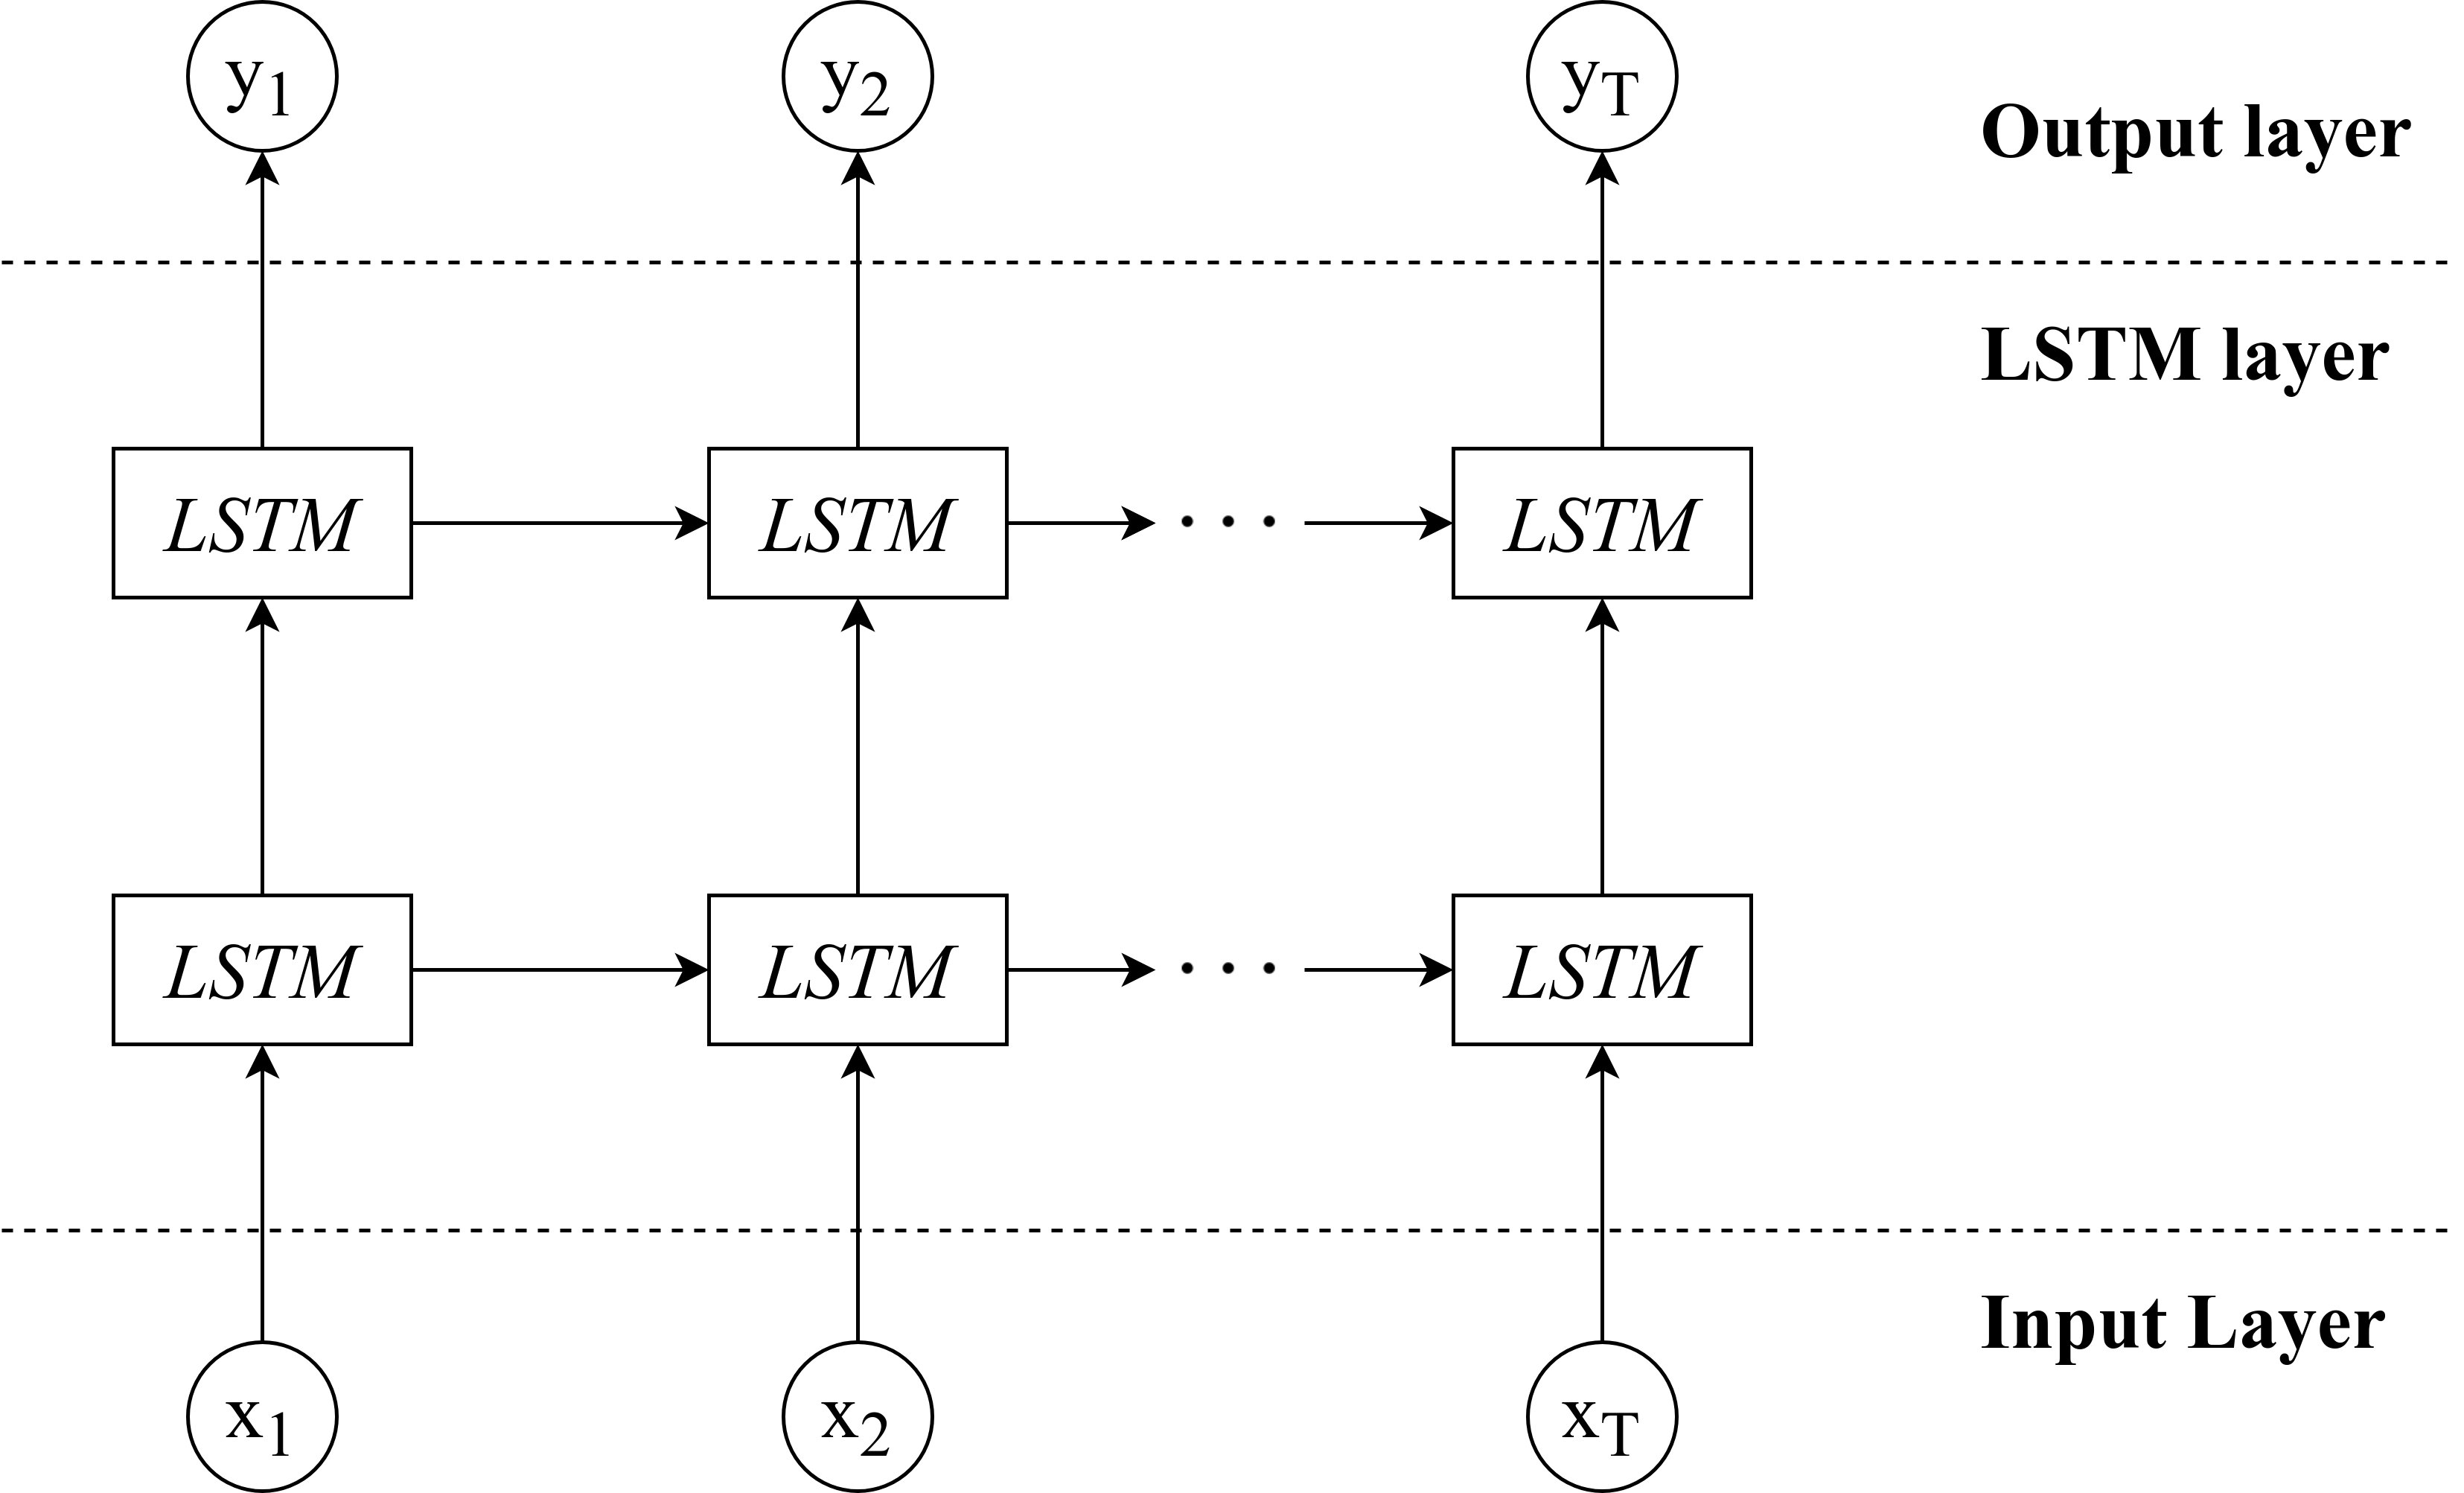
\includegraphics[width=0.6\linewidth]{\FigsDir/LSTM.png}
  \end{center}
  \caption{LSTM network \citep{QoEModel_LSTM} for the user's instantaneous QoE prediction. The network is composed of two LSTM (Long Short-term Memory) layers. The inputs to the layers are four features including STSQ, PI, NR, and TR. The outputs combine the LSTM layers' hidden states, representing the predicted instantaneous QoE values.}
  \label{fig:LSTM}
\end{figure}

\subsection{Memory Effects} \label{section:MemoryEffects}
Memory effects refer to the influence of historical/past experiences on the perceived video quality. Primacy and recency are two common effects which were investigated in numerous studies \cite{QoEModel_LSTM, QoEModel_TVQoE_ContinuousTimeQoE, QoEModel_NARX_DynamicNetworks}. In addition to these factors, the effect of forgetting curve characteristic and repetition are also considered in our proposed model.
%for the improvement of accuracy
The next parts of this subsection will discuss the role and mathematical function of these factors. Based on that, a memory weight is proposed for the cumulative QoE model.

%/====================================================================================
\subsubsection{Primacy Effect}
%/====================================================================================

The primacy effect \cite{SerialPositionEffect_FreeRecall, PrimacyVsRecency} describes the human behavior to recall (bitrate or rebuffering) initial events occurred at the beginning of the streaming session when providing the overall evaluation \cite{RehearsalProcessesInFreeRecall}. In fact, the primacy effect always exponentially decreases by time \cite{SerialPositionEffect_FreeRecall}. Therefore, its characteristics can be expressed by an exponential curve as follows:
    
\begin{equation} \label{eqn:Primacy}
  f_{P}(t) = exp(-\alpha_{P}*t), \quad 0 \leq t \leq L
\end{equation}
where $\alpha_{P}$ determines the \textit{intensity} of primacy effect (how fast the primacy effect diminishes over time) and $t$ denotes a time instant within a session of $L$ seconds.


%/====================================================================================
\subsubsection{Recency Effect}
%/====================================================================================

The recency effect \cite{SerialPositionEffect_FreeRecall,PrimacyVsRecency} refers to the ability of the human memory to recall the most recent events \cite{RehearsalProcessesInFreeRecall}, hence, the evaluated QoE heavily depends on the recent experiences. The recency effect also can be described by an exponential curve represented by the following equation:
    
\begin{equation} \label{eqn:Recency}
  f_{R}(t) = exp(-\alpha_{R}*(L - t)), \quad 0 \leq t \leq L
\end{equation}
where $\alpha_{R}$ determines the \textit{intensity} of recency effect.
    
The primacy effect and the recency effect can be combined as the U-shaped form \cite{PrimacyVsRecency}, quantifying the influenced weight of the events occurring from the beginning to the end of a video session. As shown in Figure\,\ref{fig:PrimacyRecencyShape}, it can be observed that both Eq. \ref{eqn:Primacy} and Eq. \ref{eqn:Recency} reflect the primacy and recency effect extremely well.
    
\begin{figure}[tb]
  \begin{center}
    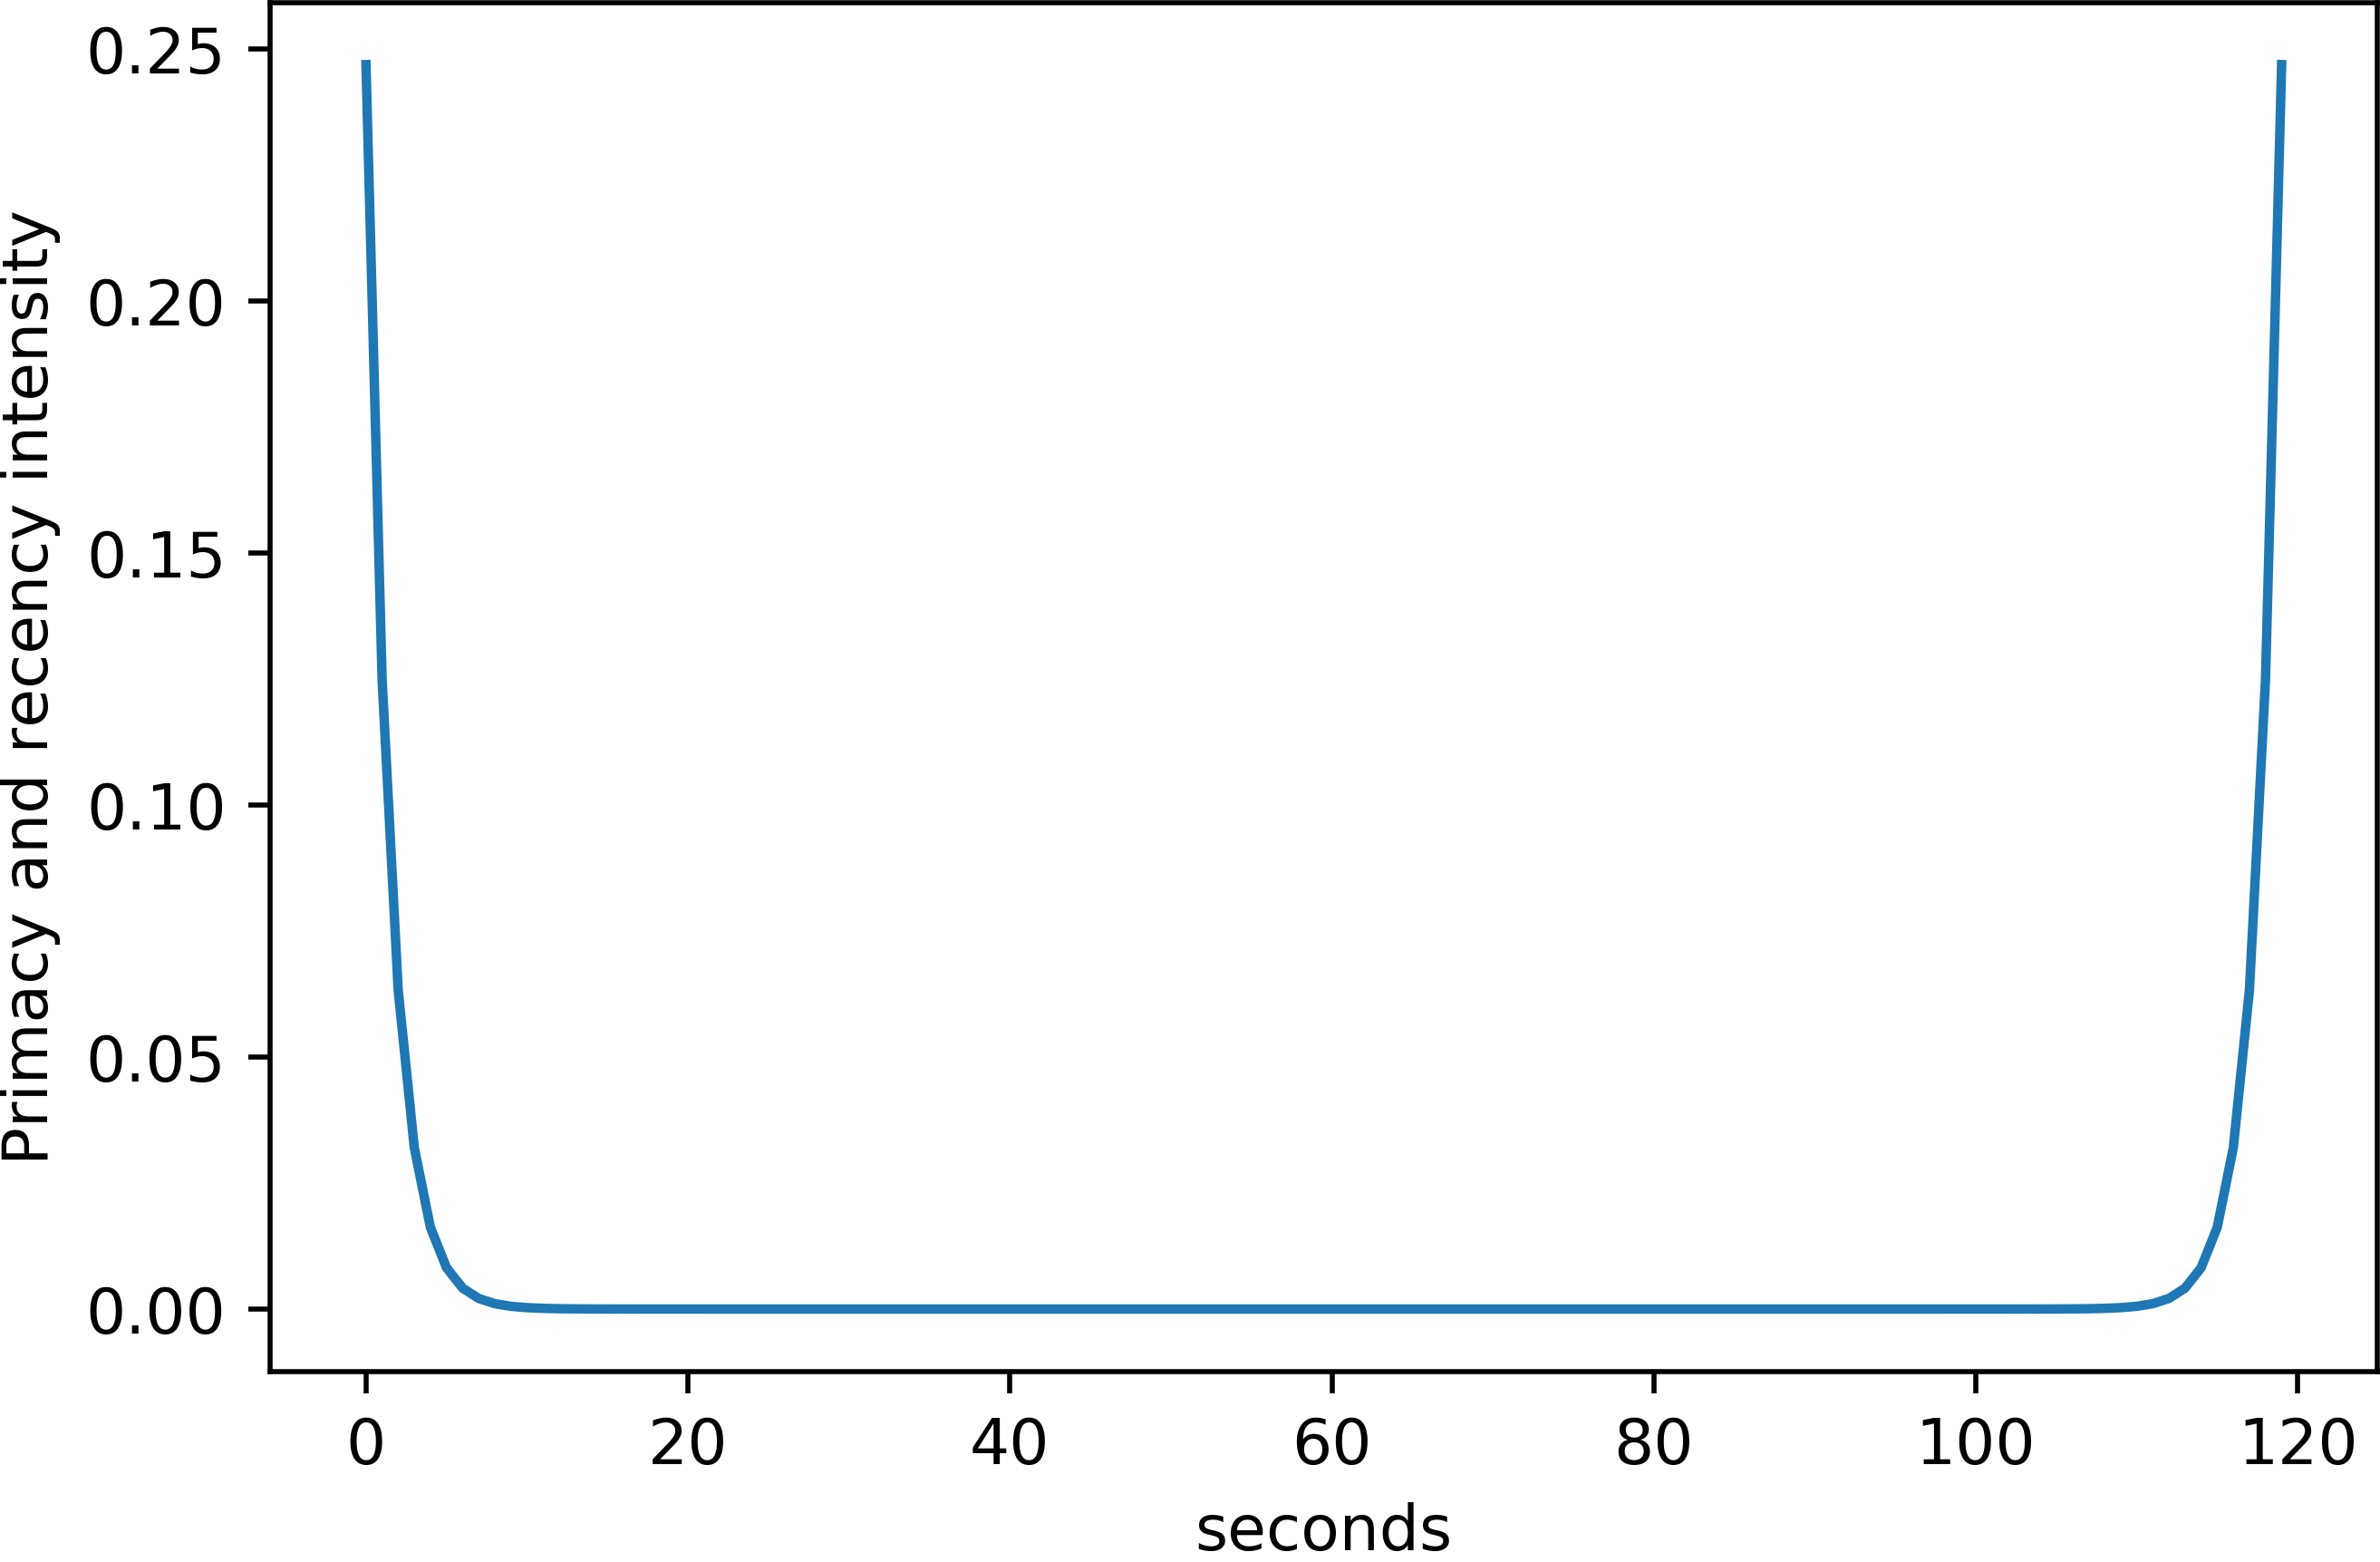
\includegraphics[width=0.6\linewidth]{\FigsDir/weight_ideal.png}
  \end{center} 
  \caption{A typical U-shaped curve combined primacy and recency effects.}
  \label{fig:PrimacyRecencyShape}
\end{figure}


%/====================================================================================
\subsubsection{Forgetting Curve and Repetition}\label{pro_for-rep}
%/====================================================================================

\begin{figure}[tb]
  \centering
  \begin{subfigure}[b]{0.49\linewidth}
    \centering
    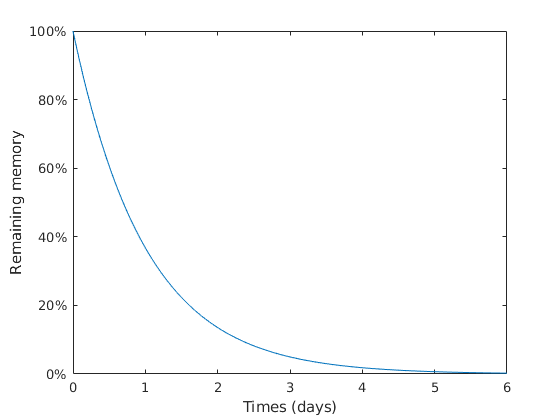
\includegraphics[width=\linewidth]{\FigsDir/forgetting_curve.png}
    \caption{An example of forgetting curve}
    \label{fig:ForgettingCurve}
  \end{subfigure}
  \hfill
  \begin{subfigure}[b]{0.49\linewidth}
    \centering
    \includegraphics[width=\linewidth]{\FigsDir/repetition_redraw.png}
    \caption{Forgetting curve and repetition}
    \label{fig:ForgettingCurveRepetition}
  \end{subfigure}
  
  \caption{Examples of forgetting curve and repetition.}
  \label{fig:ForgettingCurveRepetitionExamples}
\end{figure}

%Human memory is complex; thus, 
Due to the significant impact of the negative experience caused by distorted events, the primacy and recency effect can be neglected under repeated bitrate switches or rebuffering \cite{EffectSizesOfInfluenceFactors}. In such situations, forgetting behavior and repetition should be taken into account. The forgetting behavior, in other words, forgetting curve characteristic \cite{Ebbinghaus_ForgettingCurve} is a natural process, describing the exponential loss of memory over time. As shown in Figure \ref{fig:ForgettingCurve}, when information is learned, its memory retention declines at an exponential rate. Accordingly, any occurred events can be exponentially forgotten by time if there is no attempt to retain it. The level of remaining memory about such events at a specific time point depends on:

\begin{itemize}
  \item The strength of memory (memory intensity): The durability that memory traces in the brain. The more annoyance the event is, the stronger the user memorizes it and the longer it lasts.
  \item The time has elapsed since the occurrences of events: As shown in Figure\,\ref{fig:ForgettingCurve}, the user will forget an average of 60\% of what they experience within the first period of time \cite{EvaluatingForgettingCurves,Ebbinghaus_ForgettingCurve}.
  \item Repetition: The more frequently an event occurs, the more likely it sticks to the user memory (shown in Figure\,\ref{fig:ForgettingCurveRepetition})
\end{itemize}

In a typical streaming session, an interruption (bitrate switching or rebuffering) can happen regularly. When an event, especially rebuffering repeatedly occurs, the strength of memory of those events will trendily increases \cite{Ebbinghaus_ForgettingCurve}, negatively influencing the perceived video quality. Consequently, as the number of negative events increases, QoE will recover at a slower pace after the occurrence of each event. Such memory characteristics can be formulated as the following equation \cite{TwoComponentsOfMemory}:
    
\begin{equation} \label{eqn:Repetition}
  f_{RP}(t) = exp(-\frac{\alpha_{RP}}{NR(t)} * TR(t)), \quad 0 \leq t \leq L
\end{equation}
where $NR(t)$ is the number of rebuffering events occurring until the time $t$, $TR(t)$ is the time elapsed since the last video impairment, and $\alpha_{RP}$ is the intensity of memory related to a rebuffering event. The ratio $\frac{\alpha_{RP}}{NR(t)}$ determines the retention of the user's memory after the $NR(t)$-th rebuffering. Accordingly, the lower $\frac{\alpha_{RP}}{NR(t)}$ is, the higher retention rate, making $f_{RP}$ declines at a lower rate. 


%/====================================================================================
\subsubsection{Proposed Memory Weight}
%/====================================================================================

As discussed in the previous sub-subsections, the effects of primacy, recency, forgetting behavior and repetition are significantly crucial for the evaluation of the cumulative QoE. Therefore, in the proposed cumulative QoE model, we introduce a novel \textit{memory weight} incorporating the effects of those factors to accurately assess the cumulative human perception during a streaming session. The proposed memory weight is represented by Eq. \ref{eqn:Weight}. An example of time-varying memory weight is illustrated in Figure \ref{fig:ForgettingCurveRebuff}. In fact, Eq. \ref{eqn:Weight} is a linear combination effect of the above-mentioned memory factors obtained from Eq. \ref{eqn:Primacy}, Eq. \ref{eqn:Recency} and Eq. \ref{eqn:Repetition}.
    
\begin{equation} \label{eqn:Weight}
  w_{t} = \beta_{1}f_{P}(t) + \beta_{2}f_{R}(t) + \beta_{3}f_{RP}(t)
\end{equation}

\begin{figure}[tb]
  \begin{center}
    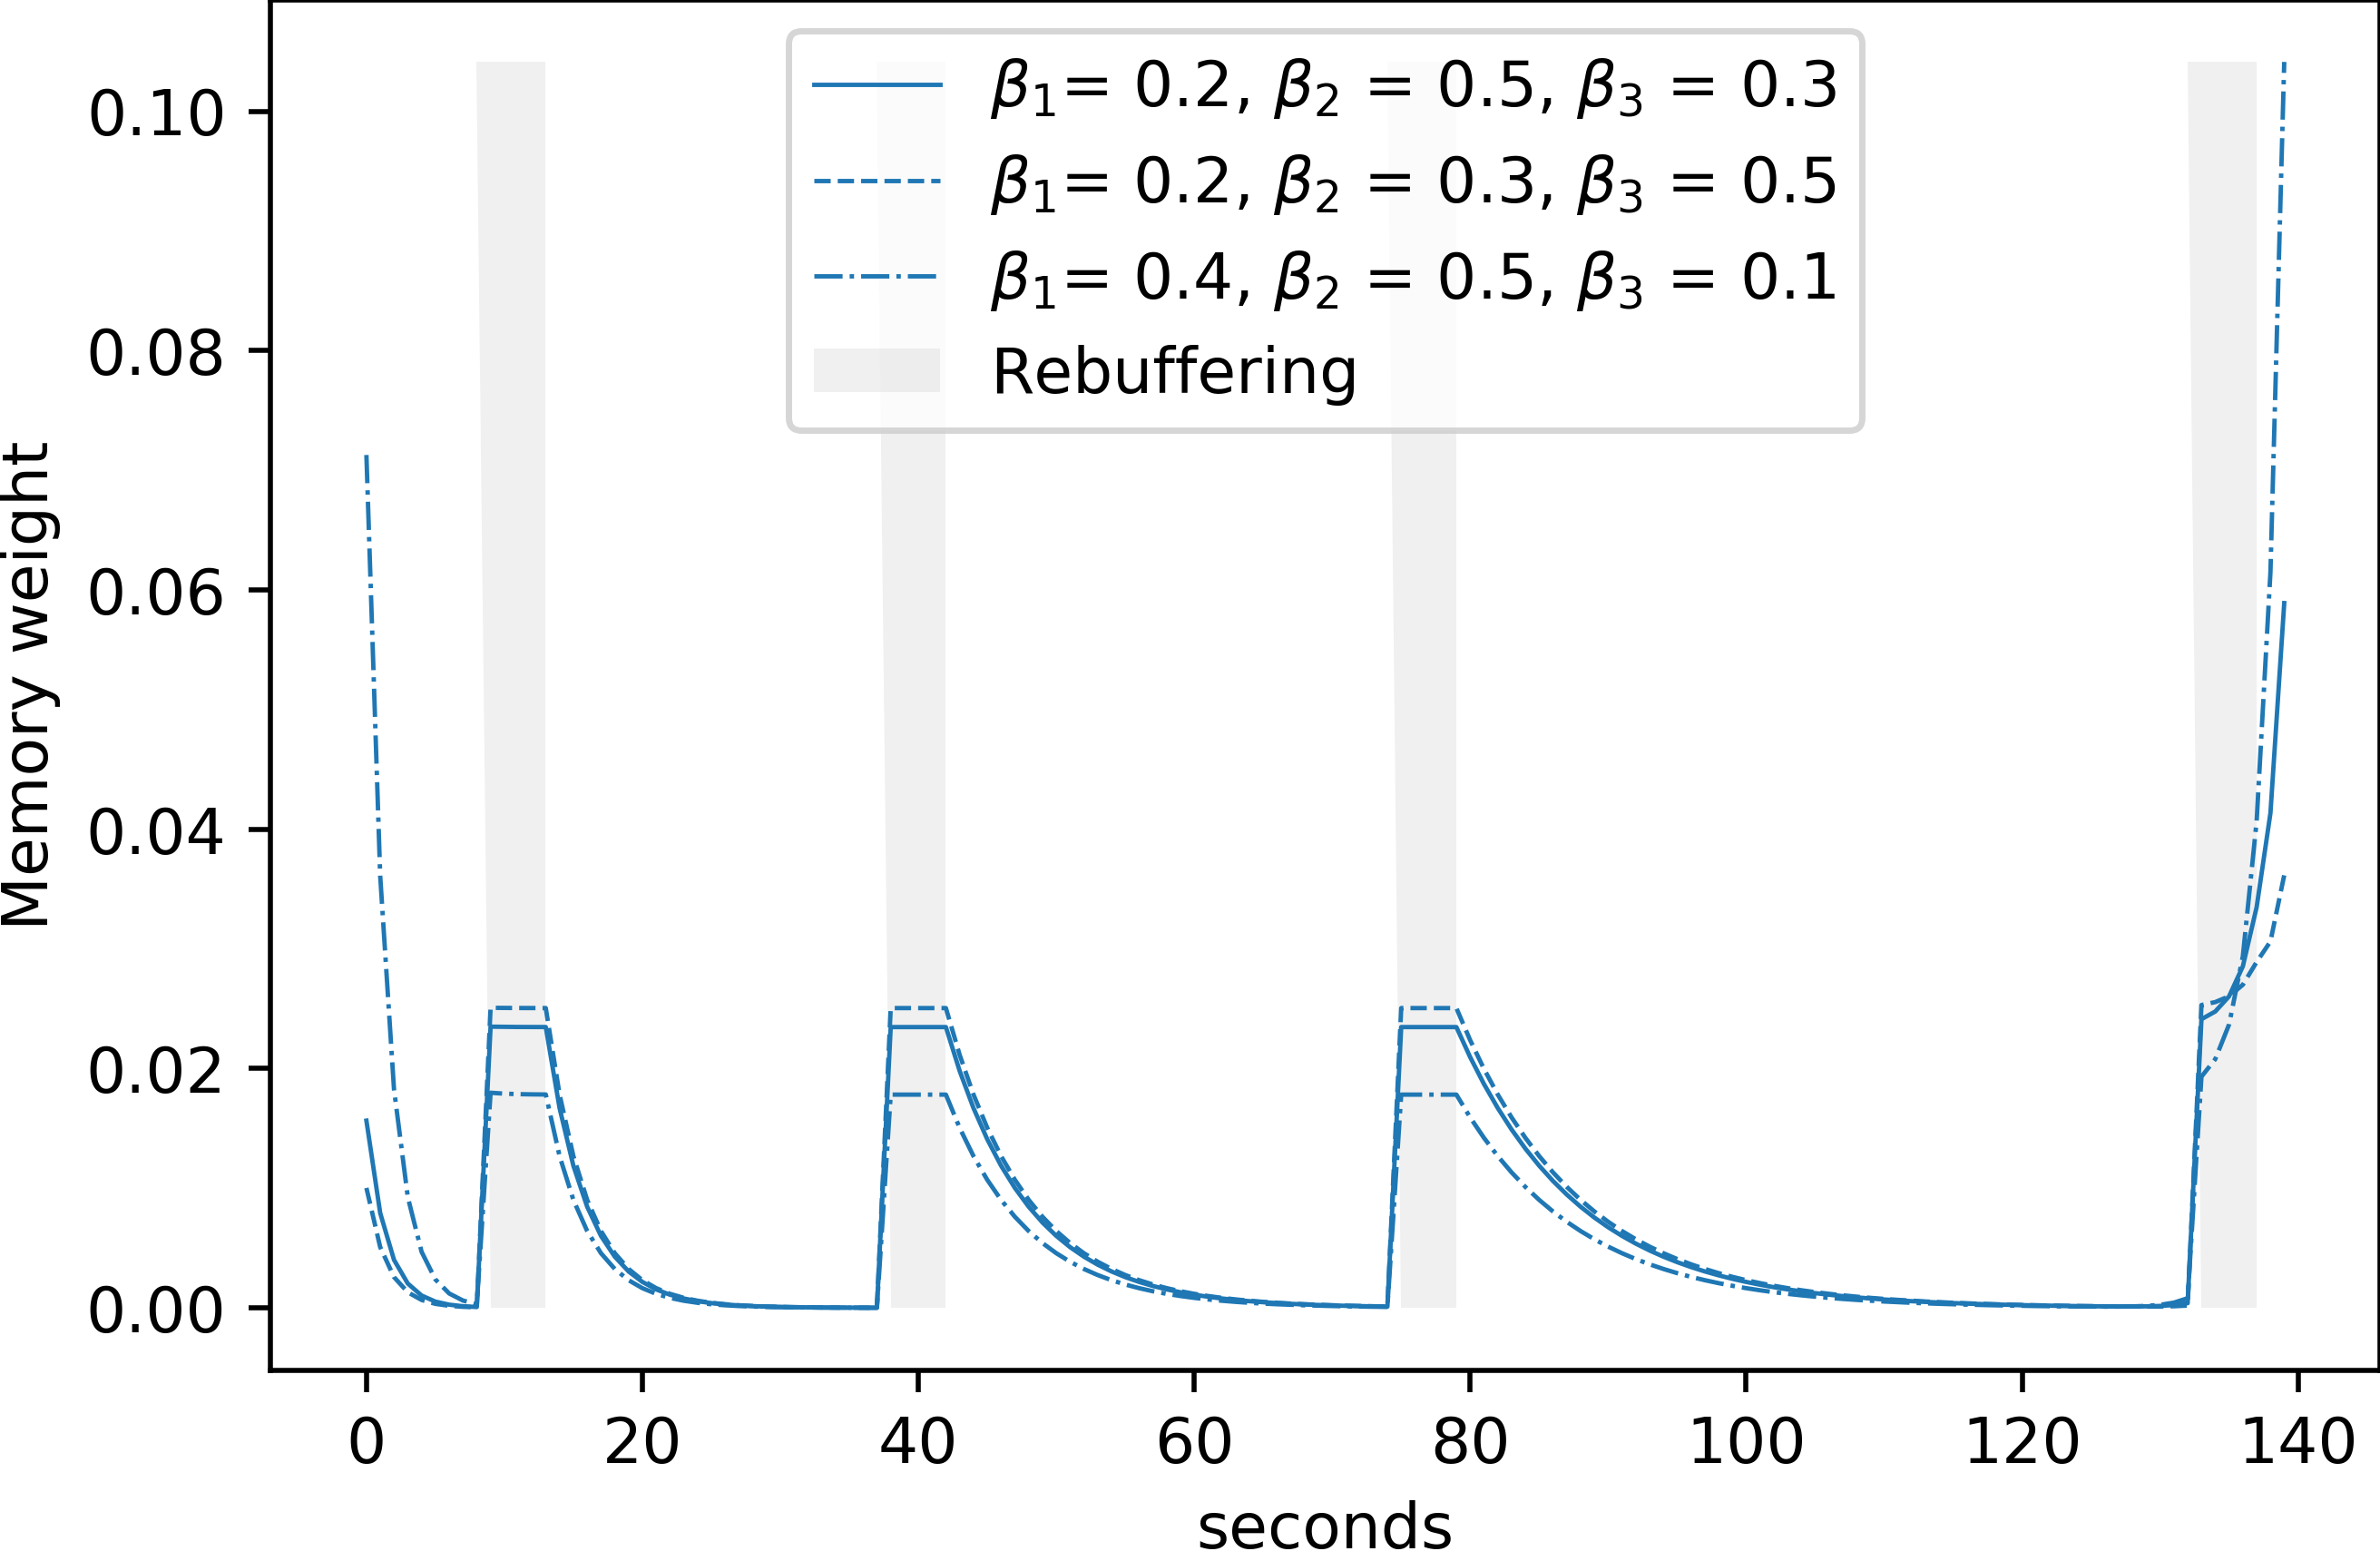
\includegraphics[width=0.7\linewidth]{\FigsDir/weight_different_params.png}
  \end{center} 
  \caption{An example of the memory weight in a session under different values of parameters $\beta_{1}$, $\beta_{2}$, and $\beta_{3}$}
  \label{fig:ForgettingCurveRebuff}
\end{figure}


where $\beta_{1},\beta_{2},\beta_{3}$ respectively determine the contribution of primacy effect, recency effect and repetition to the memory weight.

Figure. \ref{fig:ForgettingCurveRebuff} shows that when an rebuffering event occurs near the end of the session, the recency effect has a stronger effect on human perception. Therefore, in this period of times, the end user's QoE will drops dramatically. In addition, the forgetting rate of a specific interruption is also smaller than those of previous ones, determining the characteristics of forgetting behavior and repetition. Therefore, the proposed memory weight potentially reflects the intensity of human memory over time during a streaming session.


\subsection{Degree-of-Interest} \label{section:DoI}
For modeling QoE, there have been numerous studies that take into account video content-related factors (e.g., type of video, the complexity of video, etc.). However, most of them neglected the user's interest, in other words, DoI. In fact, influenced by video content and viewer preferences, the user possibly has different DoI on different videos or different parts of a video. Intuitively, the user seems to provide higher QoE scores for the video with interesting content and vice versa. Typically, Degree-of-Interest (DoI) \cite{DegreeOfLiking_SOS} is defined as the interestingness of the video content, or the ability of the video content to attract the user and keep the user's interest \cite{VisualContent}.

To make this clear, we investigate the correlation between DoI and the overall QoE by conducting a subjective test. In this test, 18 undistorted videos from the LFOVIA Database \cite{LFOVIA} were utilized. The video content varied upon nature, wildlife, outdoor, marine, sports, animation, and gaming \cite{LFOVIA} among every video, each of which the duration is 120 seconds. This guaranteed that the subjects would retain their interests as they watched.
%The snapshots of these videos are shown in Figure \ref{fig:snapshots}.
The referenced videos were randomly divided into 6 collections and encoded using FFmpeg \cite{FFmpeg} under the default settings with the resolution of 1920 x 1080 and were displayed on a 15-inch monitor with a resolution of 1920 x 1080 and a black background. The Absolute Category Rating (ACR) \cite{ITUT_P913} method was used and there were 60 subjects agreed to participate in this experiment. Each video was assessed by at least 10 subjects. At the end of each video, the subject was asked to give an overall score representing his/her interest in the entire video content, ranging from 1 (worst or not at all interested) to 5 (best or extremely interested), following the general principle of the ITU-T recommendation P.913 \cite{ITUT_P913}. A 3-minute break was provided to each subject between each video to minimize the effects of viewer fatigue. The average of subjects' scores or Mean Opinion Score (MOS) for each video was utilized as the DoI of video. These values were then linearly scaled up to the range of 0 to 100 and compared with the corresponding overall QoE in the LFOVIA Database.

\begin{figure}[tb]
  \begin{center}
    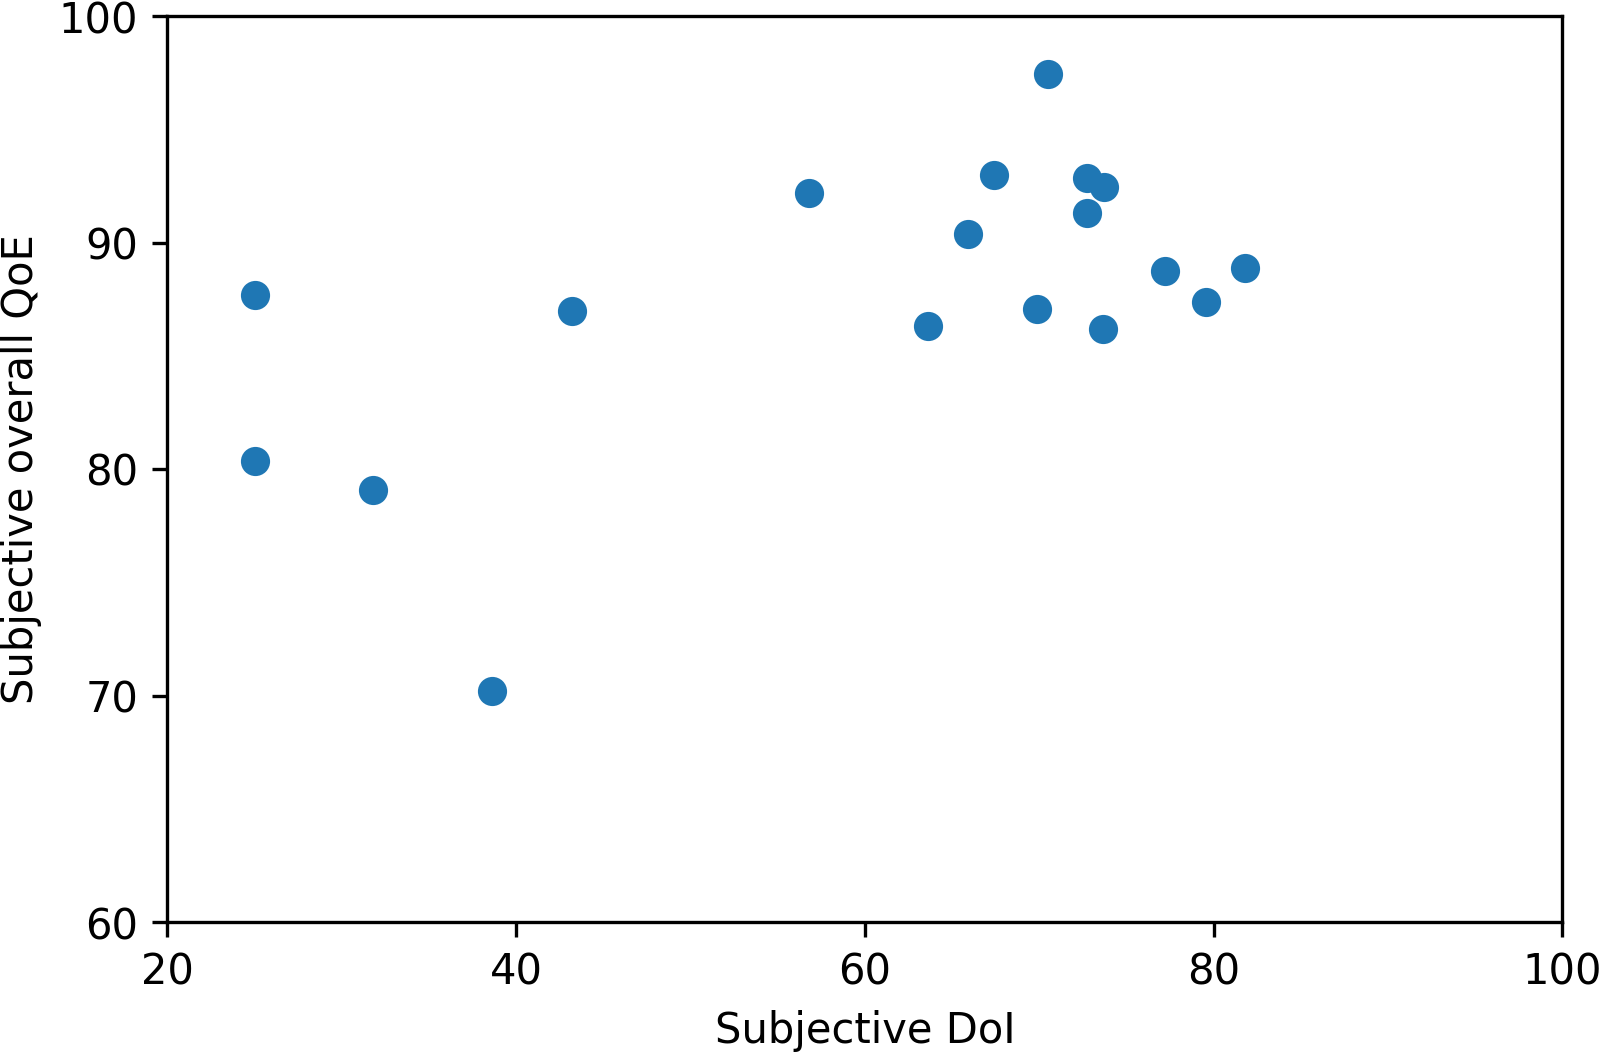
\includegraphics[width=0.6\linewidth]{\FigsDir/pcc_doi_overallqoe.png}
  \end{center}
  \caption{Scatter plot between the mean of subjective DoI scores and the subjective overall QoE obtained in the database.}
  \label{fig:PCC_DoI_OverallQoE}
\end{figure}

Figure \ref{fig:PCC_DoI_OverallQoE} illustrates the obtained correlation between DoI and the overall QoE, which achieved the Pearson Correlation Coefficient (PCC) of \textbf{0.601}. The correlation was modest. We speculate this as the small number of subjects participating in the experiment. Yet, it is shown that the DoI has an influence on the final decisions of the users when they provide the overall QoE. In the future, a larger number of subjects will be considered for further investigation. Based on the conclusion of this experiment, we introduce DoI as one of the potential influence factors in the proposed cumulative QoE model.


\subsection{Cumulative QoE model} \label{section:CumulativeQoE}
Through the investigation of the above human-related influence factors, the proposed cumulative QoE model is generally presented in Eq.\,\ref{eqn:Cumulative_QoE}. In this model,
to quantify how each of the user's past experiences influences the cumulative perception,
the instantaneous QoE needs to be weighted by the memory effect from the beginning of playback to the investigated time point $t$ within a streaming session.
According to our proposed model, the procedure of estimating cumulative QoE is described as follows: Firstly, the instantaneous QoE is predicted by LSTM-QoE model \cite{QoEModel_LSTM}, and stored into vector ${Q}_{t} = (q_{0},  q_{1}, \dots, q_{t})$. Secondly, the memory weight is calculated by the Eq.\,\ref{eqn:Weight} to form vector ${W}_{t} = (w_{0},  w_{1}, \dots, w_{t})$.

\begin{equation} \label{eqn:Cumulative_QoE}
  CQ_{t} = \lambda_{1} \left ( {Q}_{t}\times{W}^{T}_{t} \right ) + \lambda_{2}DoI
\end{equation}

where $\lambda_{1}$, $\lambda_{2}$ are correlation coefficients which respectively determine the contribution of the user's past experience and user's interest in video content to the predicted cumulative QoE $CQ_{t}$ at time instant $t$.


\section{Performance Evaluation and Discussion}
\label{Cumulative:sec:Evaluation}
\subsection{Input Features for QoE Prediction}
\label{BiLSTM:subsec:InputFeatures}


\begin{figure}[tb]
  \centering
  \begin{subfigure}{0.48\linewidth}
    \centering
    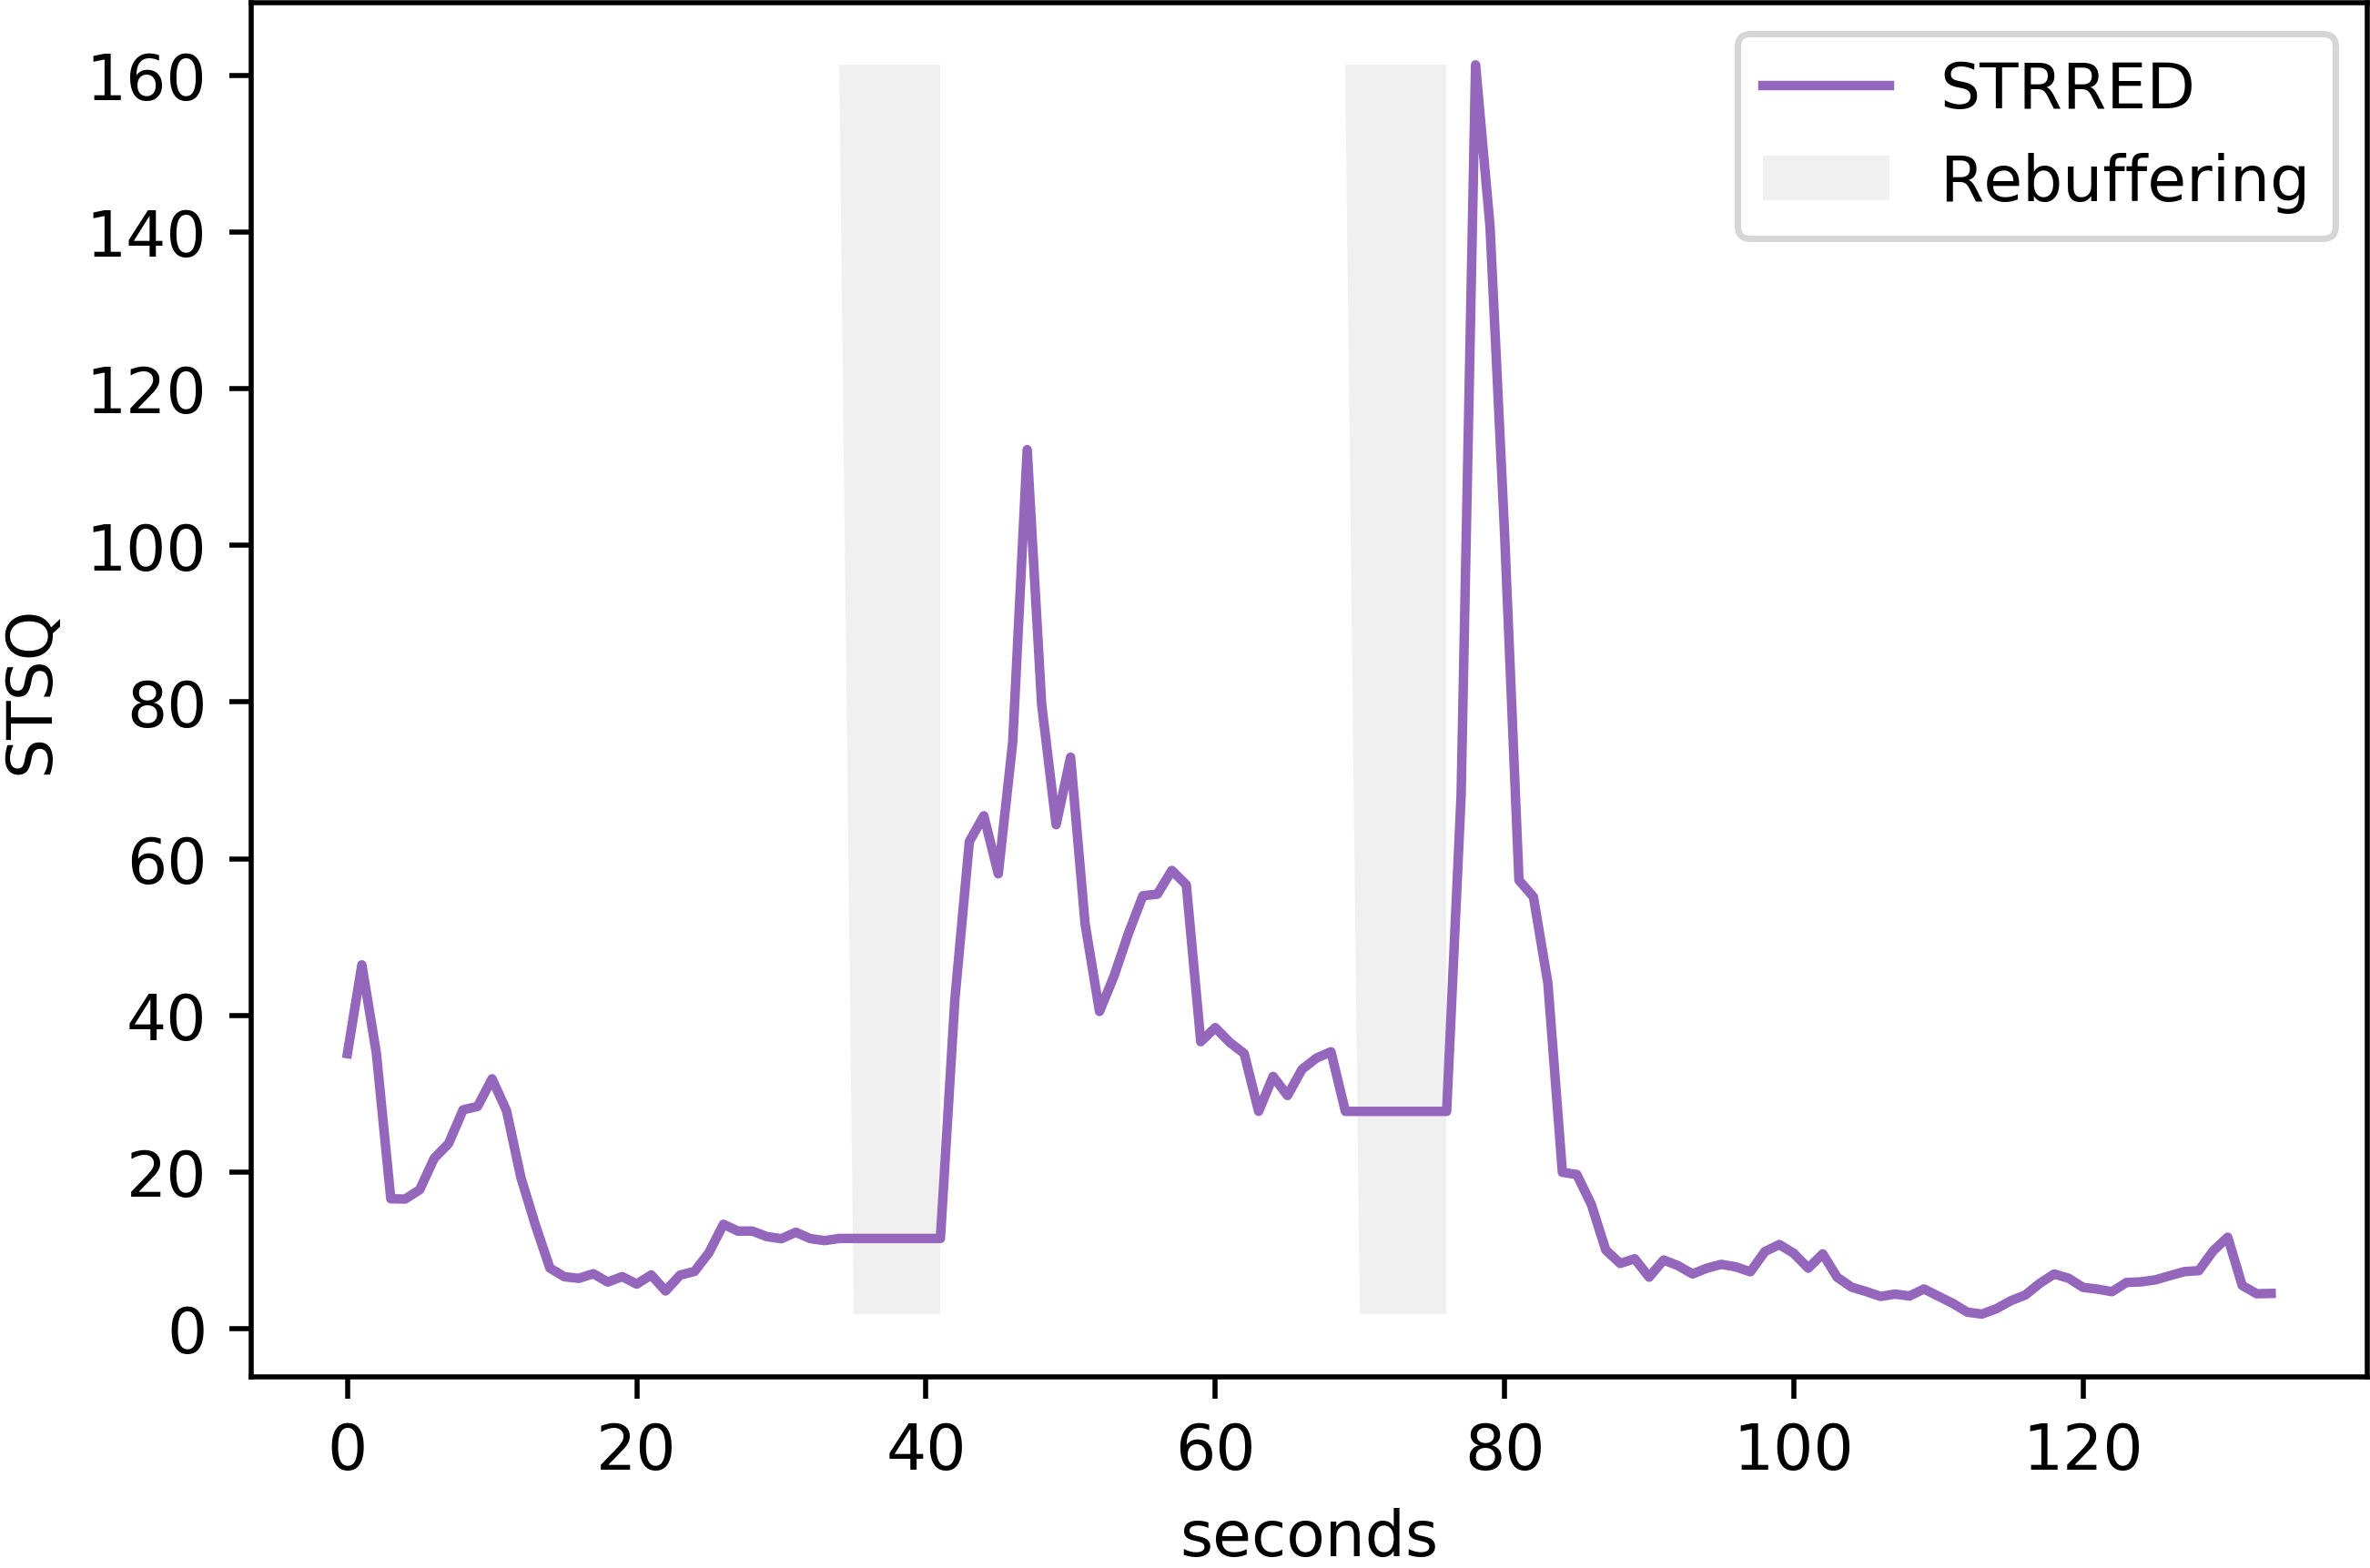
\includegraphics[width=\textwidth]{\FigsDir/features_STSQ.png}
    \caption{STSQ}
    \label{fig:InputFeatures_STSQ}
  \end{subfigure}
  \hfill
  \begin{subfigure}{0.48\linewidth}
    \centering
    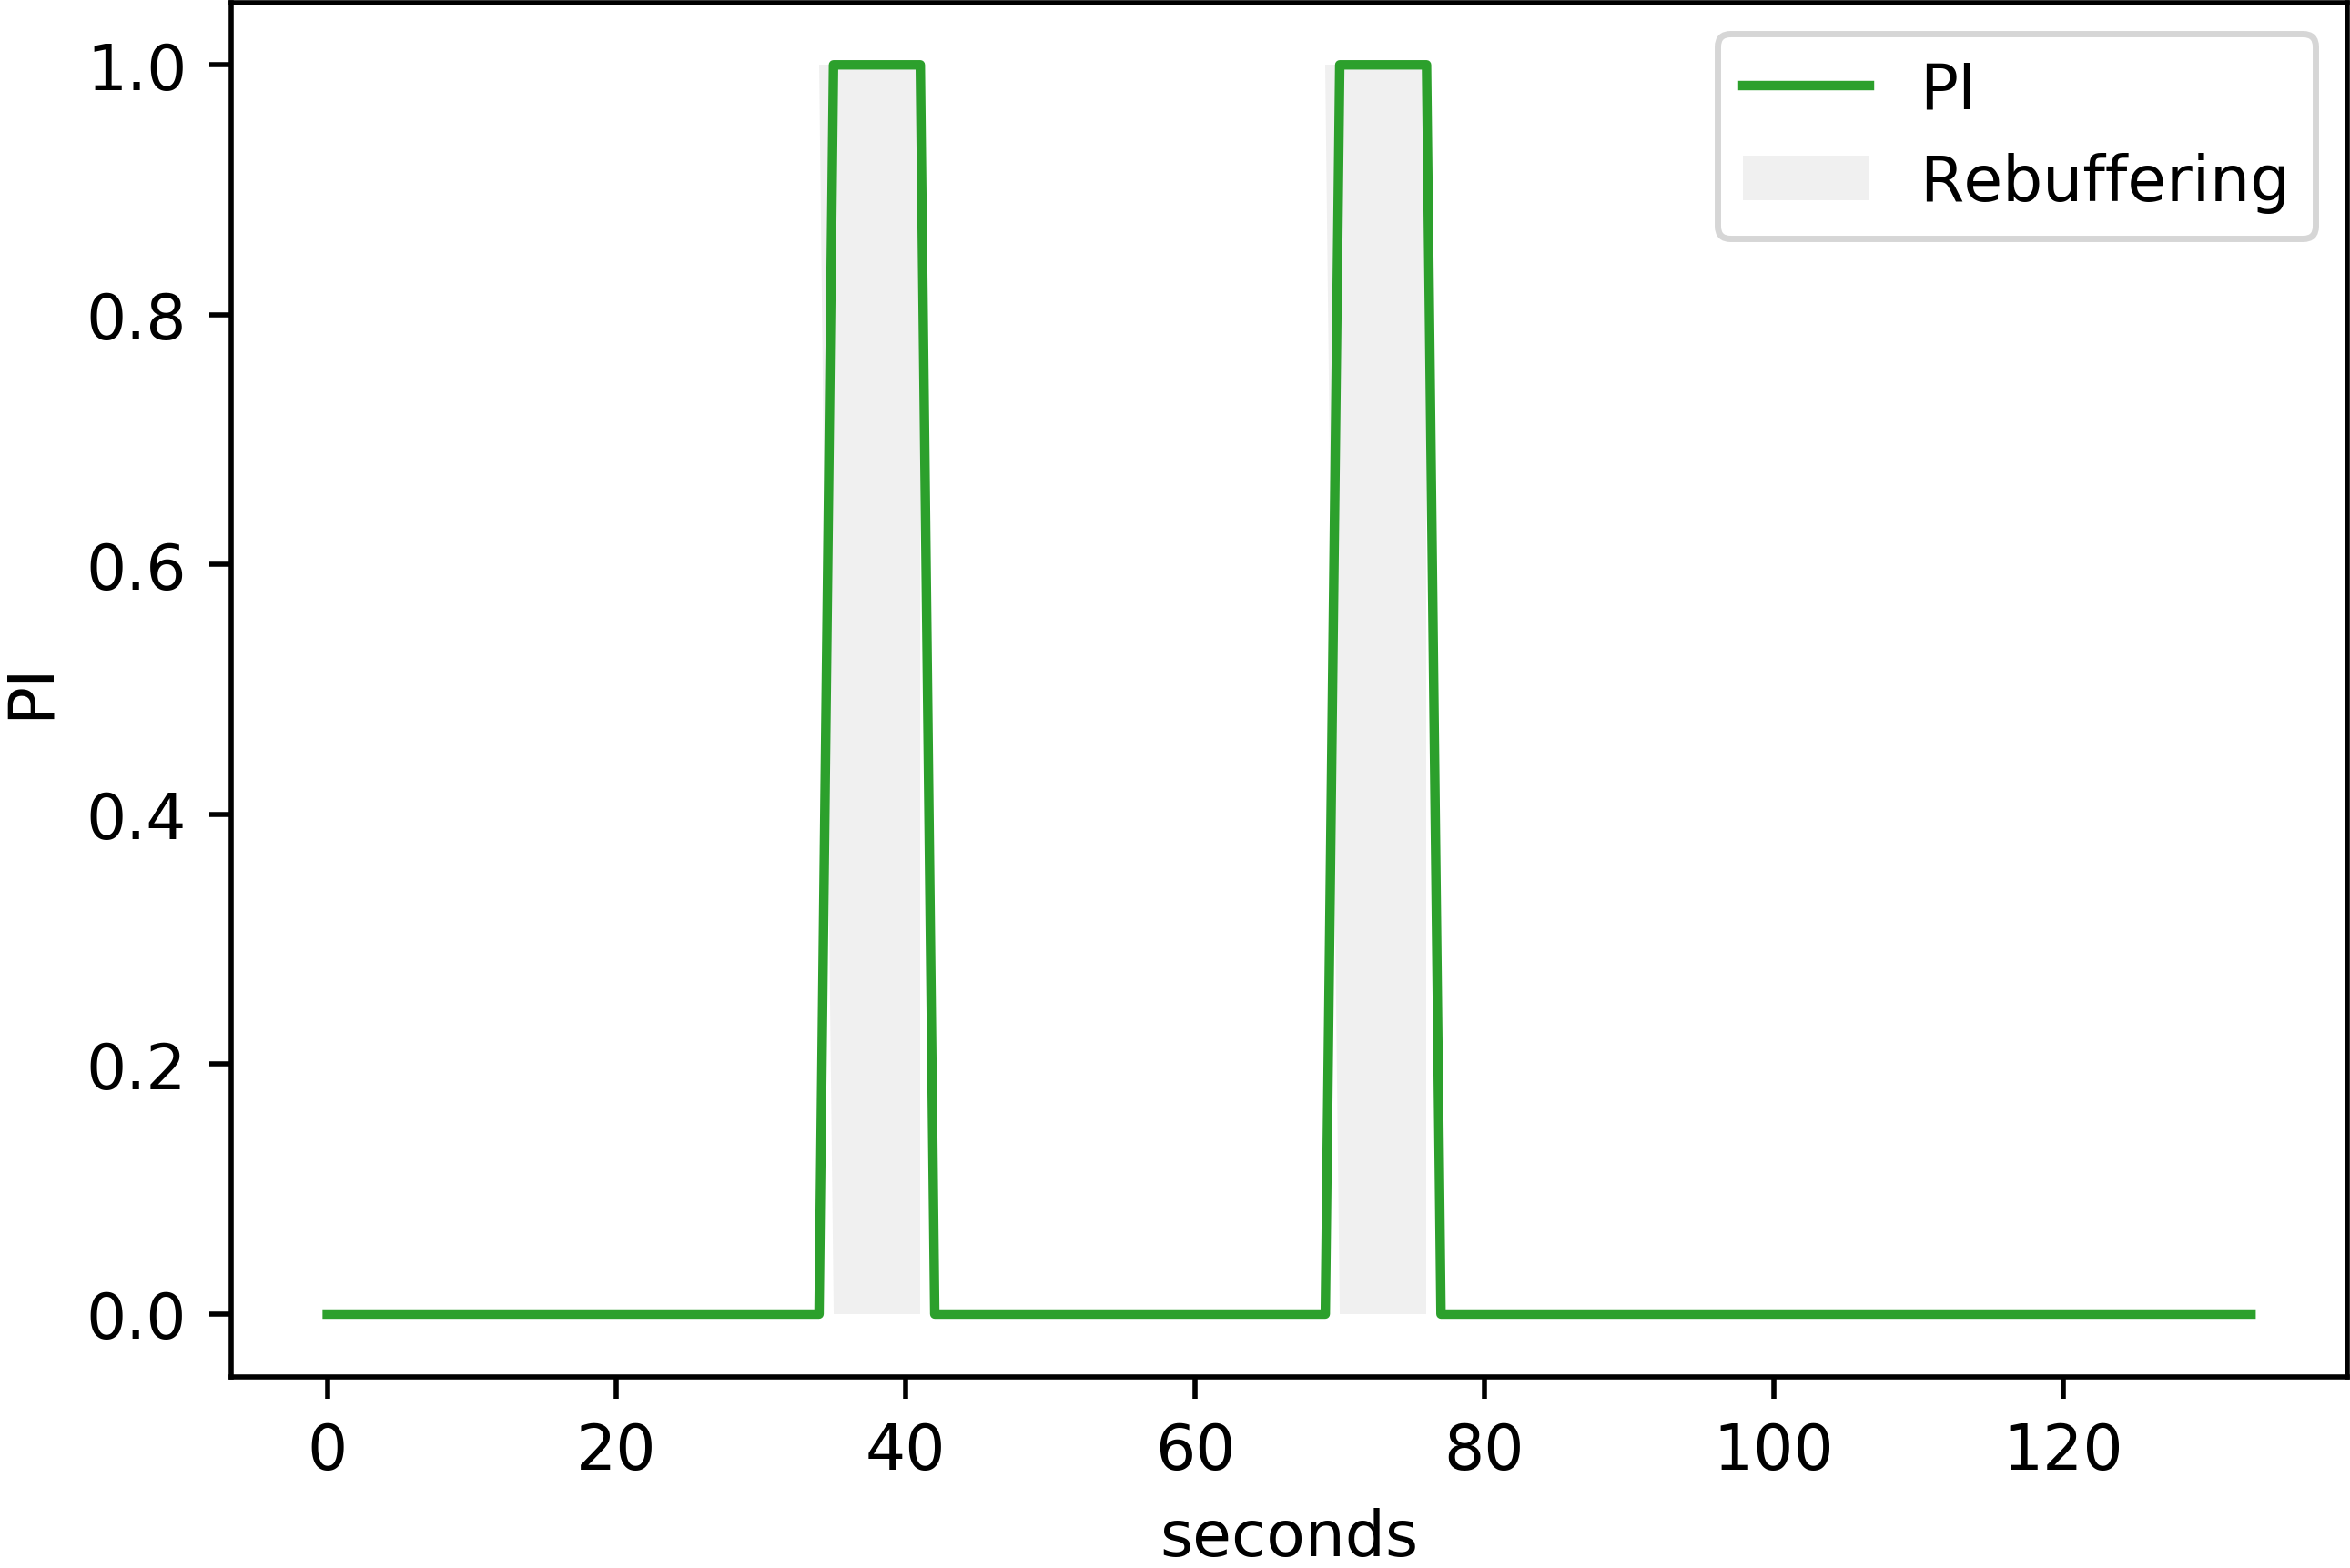
\includegraphics[width=\textwidth]{\FigsDir/features_PI.png}
    \caption{PI}
    \label{fig:InputFeatures_PI}
  \end{subfigure}
  
  \vspace{6pt}
  
  \begin{subfigure}{0.48\linewidth}
    \centering
    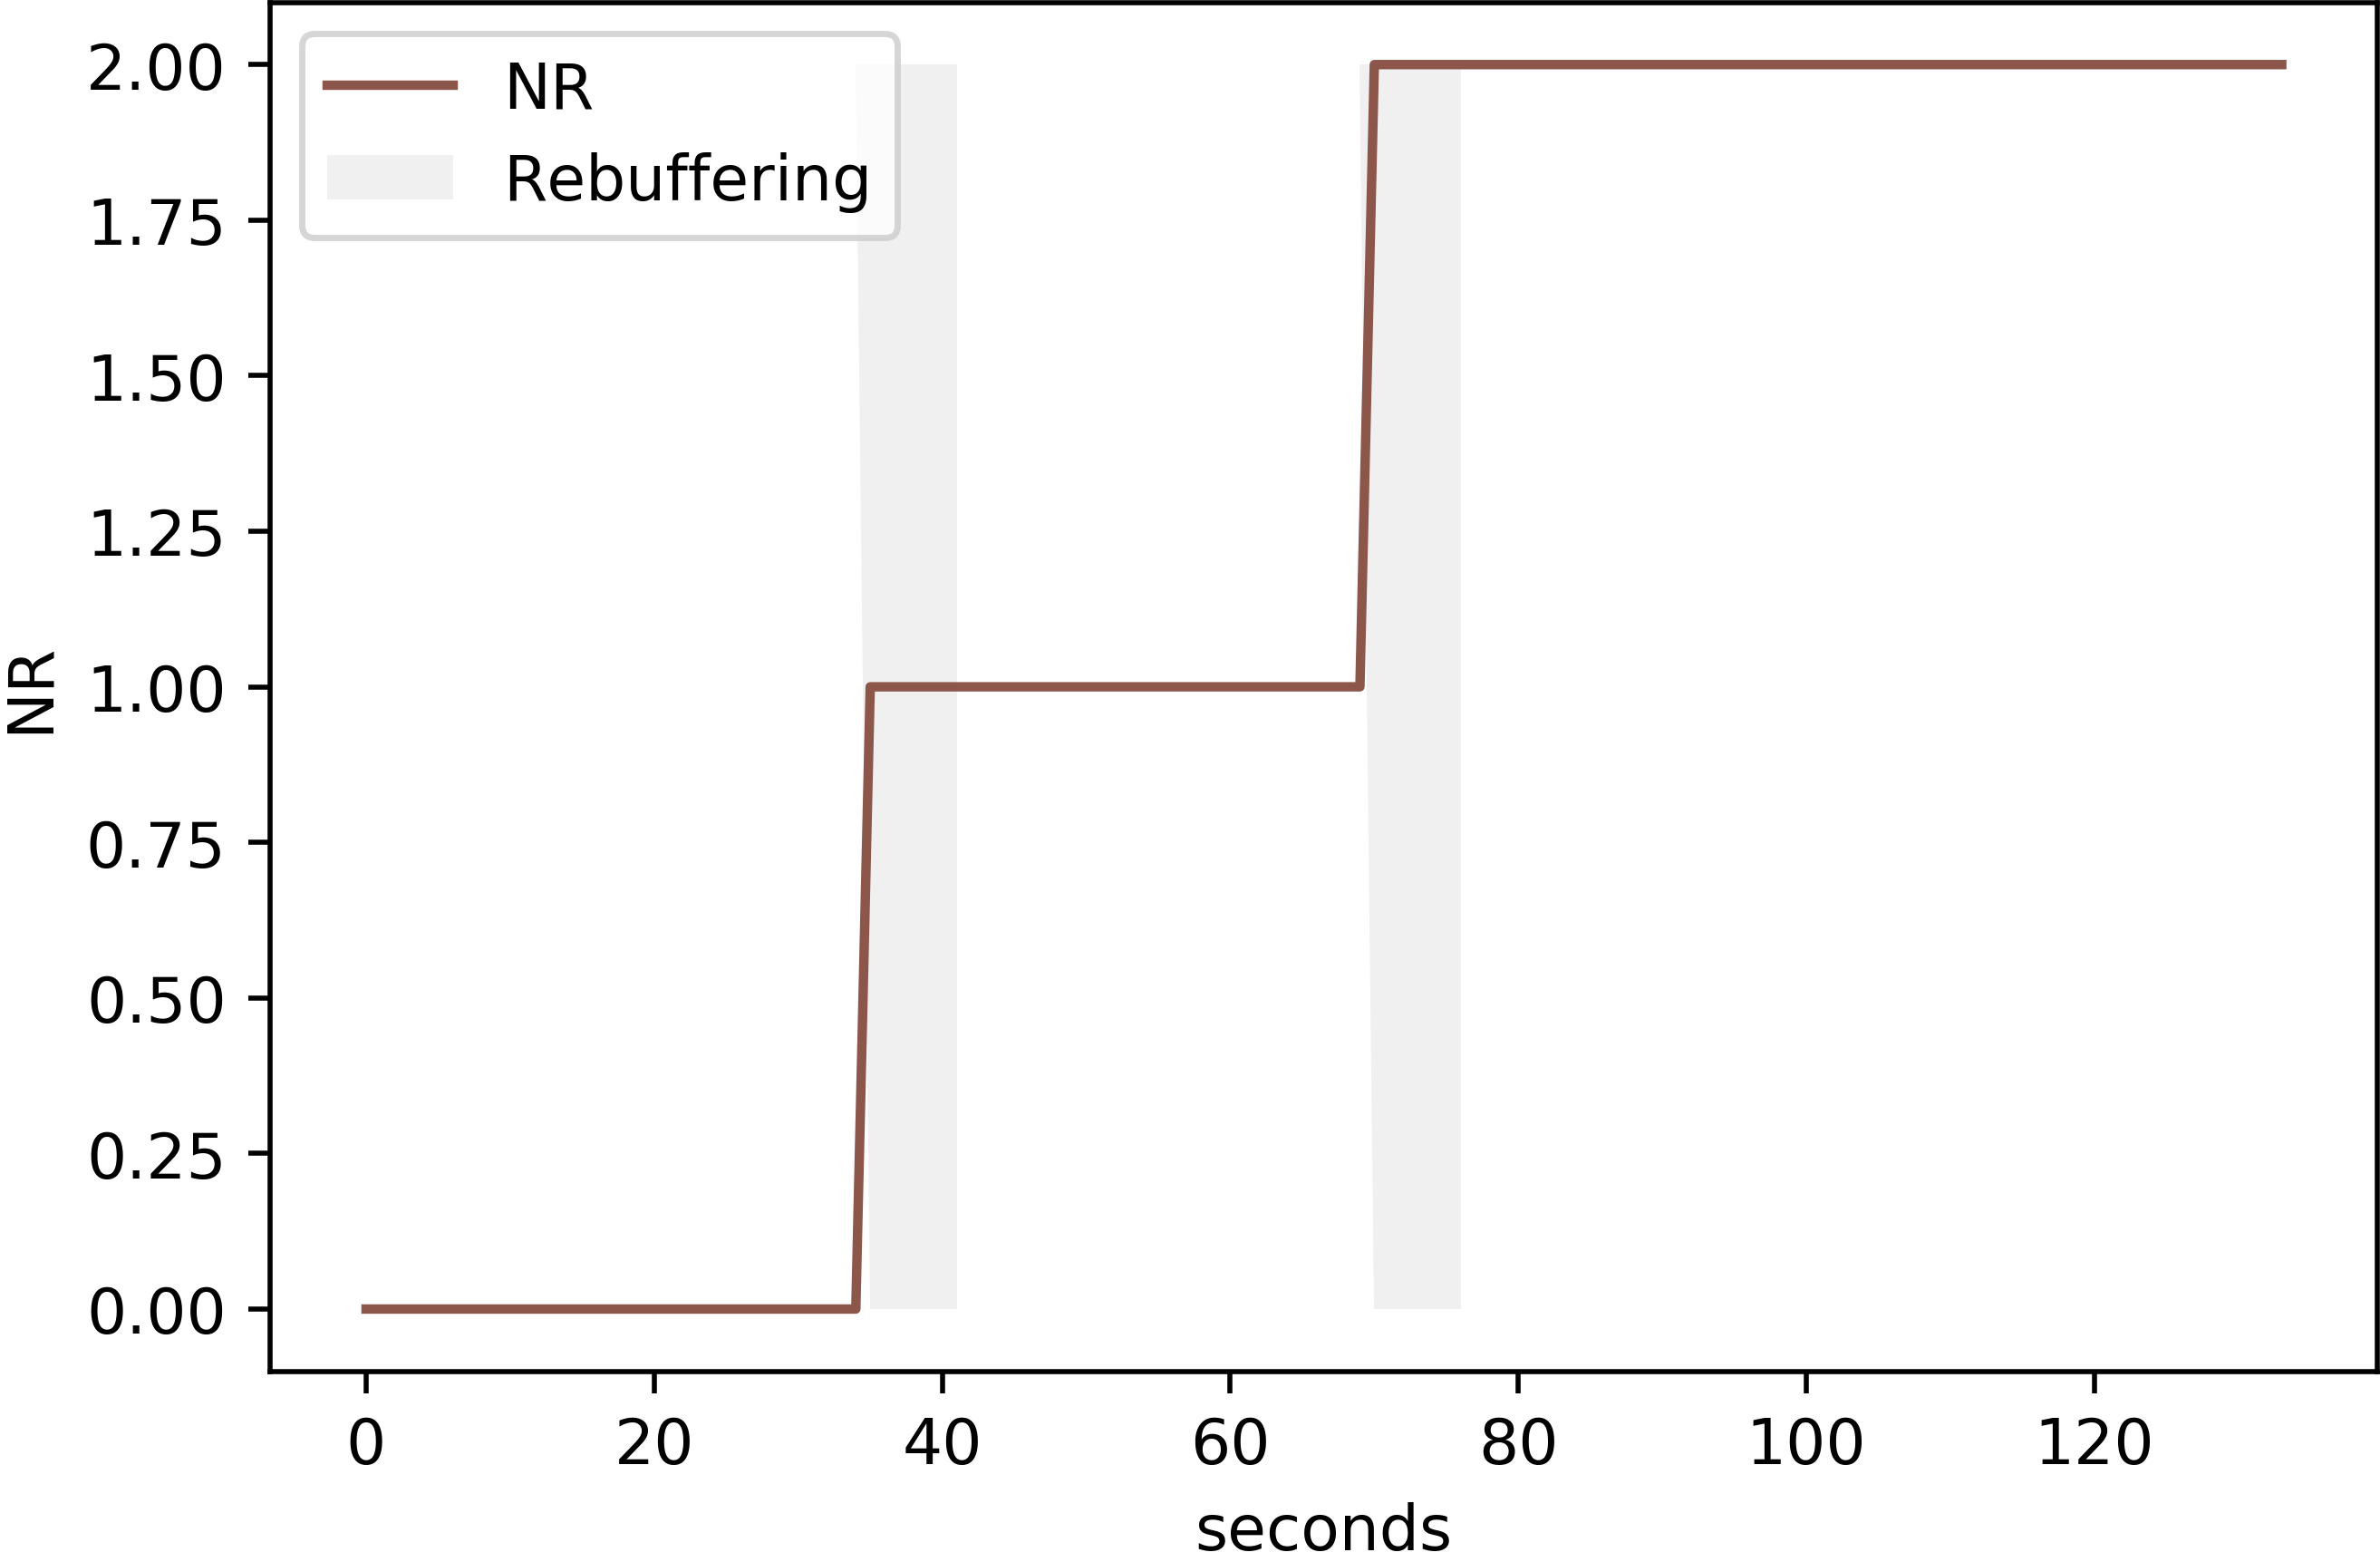
\includegraphics[width=\textwidth]{\FigsDir/features_NR.png}
    \caption{NR}
    \label{fig:InputFeatures_NR}
  \end{subfigure}
  \hfill
  \begin{subfigure}{0.48\linewidth}
    \centering
    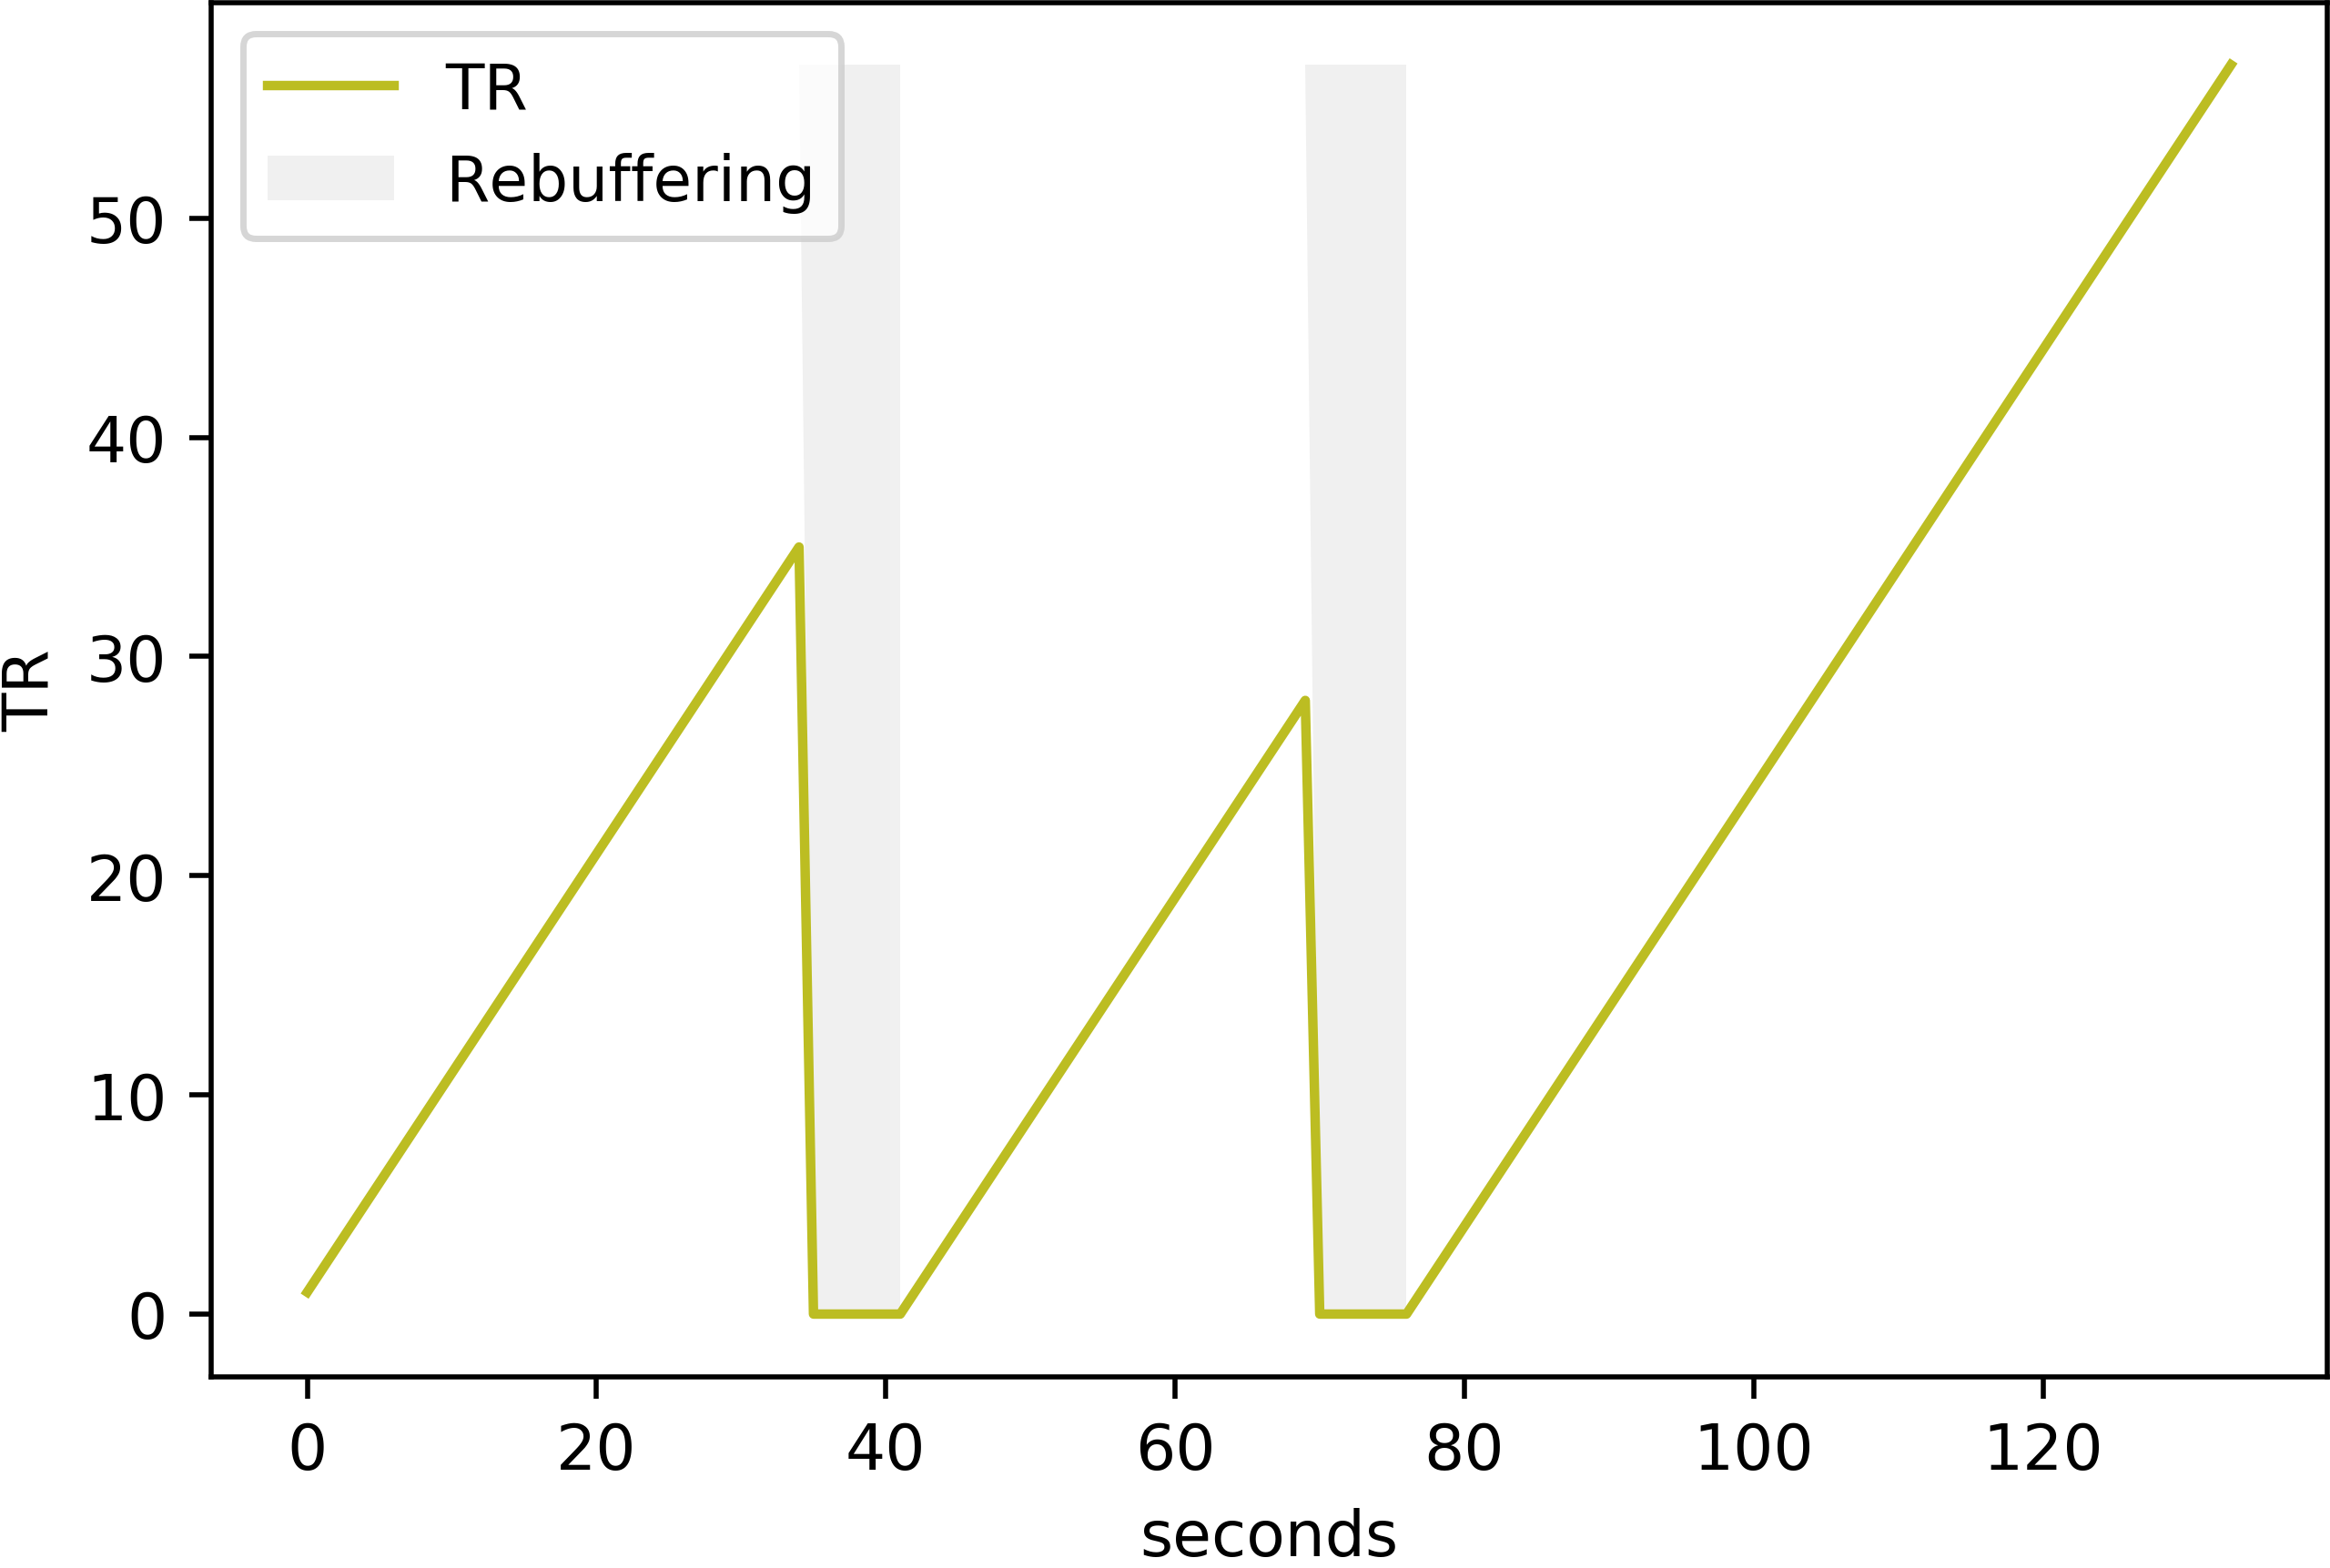
\includegraphics[width=\textwidth]{\FigsDir/features_TR.png}
    \caption{TR}
    \label{fig:InputFeatures_TR}
  \end{subfigure}
  
  \caption{Example of rebuffering and bitrate-related features represented by STSQ, PI, NR, and TR}
  \label{fig:InputFeatures}
\end{figure}


Video streaming users are sensitively affected by the video quality, known as \textit{short time subjective quality} (STSQ) \cite{QoEModel_TimeVaryingSubjectiveQuality}.
STSQ is defined as the visual quality of video being rendered to the user and can be predicted using any of the robust video quality assessment (VQA) metrics, such as Spatio-Temporal Reduced Reference Entropic Differences (STRRED) \cite{STRRED}, Multi-Scale Structural Similarity (MS-SSIM) \cite{MSSSIM}, Peak Signal to Noise Ratio (PSNR) \cite{PSNR}, etc.
Recent experiments have demonstrated that STRRED is a robust and high-performing VQA model when being tested on a very wide spectrum of video quality datasets, on multiple resolution and device types \cite{FeaturePredictionQoE, QoEModel_NLSS, QoEModel_LSTM}.
Therefore, STRRED is utilized to measure the STSQ.

Rebuffering greatly impacts the user's QoE \cite{StallingEvents}.
Thus, rebuffering information such as rebuffering length, rebuffering position and the number of rebuffering events must be investigated.
As a result, two rebuffering-related inputs are employed.
Firstly, \textit{playback indicator} (PI) \cite{QoEModel_NARX_DynamicNetworks, QoEModel_NLSS, QoEModel_LSTM} is defined as a binary continuous-time variable, specifying the current playback status, i.e., $1$ for rebuffering and $0$ for normal playback.
Secondly, as the user's annoyance increases whenever a rebuffering event occurs \cite{StallingEvents}, the \textit{number of rebuffering events} (NR) happened from the start to the current time instant of the session is considered.

Besides, the user's QoE is also affected by memory factors.
For example, more recent experiences have larger impacts on the user's perceived video quality, known as the recency effect \cite{Recency, NetflixQoE, LFOVIA}.
To capture the relation between the recency effect and the user's QoE, \textit{time elapsed since the last video impairment} (i.e., bitrate switch or rebuffering occurrence) \cite{QoEModel_NARX_DynamicNetworks, QoEModel_NLSS, QoEModel_LSTM}, denoted as TR, is utilized.


All the considered QoE influence factors are fed to the BiLSTM-QoE model to predict the instantaneous QoE. The examples of four factors (including STSQ, PI, NR, and TR) are illustrated in Figure \ref{fig:InputFeatures}.




\subsection{LIVE Netflix Video QoE Database}


The BiLSTM-QoE model is evaluated on the LIVE Netflix Video QoE Database \citep{NetflixQoE}.
The database consists of 112 distorted videos generated from 14 video contents by 8 different playout patterns
including bitrate changing, rebuffering events and mixtures of both \citep{NetflixQoE}.
The training and testing strategy are defined in \citep{QoEModel_LSTM}.
For each video $j$ in the database, one train-test set is created,
the model is trained on the set of videos that do not have the same content
and the playout pattern as the video $j$ in the test set.
Therefore, there are 112 train-test sets, each contains 1 testing videos and 91 training videos
(excludes 14 videos with the same content and 7 with the same playout pattern).
With this strategy, content and pattern dependencies are eliminated.




\subsection{Evaluation Results}


\Figure[tb][width=\linewidth]{\FigsDir/results.png}
  {QoE prediction performance of the BiLSTM-QoE over the LIVE Netflix Video QoE Database.\label{fig:BiLSTM_Accuracy}}
\Table[b]{\TablesDir/accuracy}
  {QoE prediction performance of the BiLSTM-QoE over the LIVE Netflix Video QoE Database.\label{tbl:BiLSTM_Accuracy}}


The BiLSTM-QoE model was trained and tested as described above.
The QoE prediction on the database using 4 features (i.e. STSQ, PI, TR and NR) are illustrated in Figure 6. 
The mean QoE prediction performance results are tabulated in Table \ref{tbl:BiLSTM_Accuracy},
also compared with other QoE models in the same database.
There are three considered evaluation criteria: Pearson Correlation Coefficient (PCC), Spearman Rank Correlation Coefficient (SROCC), and Root Mean Squared Error (RMSE).
The proposed model outperforms LSTM-QoE \citep{QoEModel_LSTM}, NLSS-QoE \citep{QoEModel_NLSS} and NARX \citep{QoEModel_NARX_DynamicNetworks} in terms of QoE prediction accuracy.
This is because the BiLSTM networks are very suitable to learn more useful information from time-varying features,
thereby allows this model to achieve the best performance among all the referenced models.

\section{Summary}
\label{Cumulative:sec:Summary}
\input{\SectionsDir/4_Summary}
\chapter{Discussion}
\label{ch:Discussion}


\renewcommand{\SectionsDir}{Chapter6/Sections}
\renewcommand{\FigsDir}{Chapter6/Figs}
\renewcommand{\TablesDir}{Chapter6/Tables}


This chapter discusses the QoE prediction performance of the three QoE models proposed in this thesis.
Section \ref{Discussion:sec:InstantaneousQoE} discusses the performance of two instantaneous QoE prediction models which are BiLSTM-QoE and CNN-QoE. 
Section \ref{Discussion:sec:CumulativeQoE} summarized the advantages and remaining issues of the cumulative QoE prediction model.


\section{QoE prediction performance of BiLSTM-QoE and CNN-QoE models}
\label{Discussion:sec:InstantaneousQoE}

\Table[tb]{\TablesDir/compare}
  {QoE prediction accuracy of the BiLSTM-QoE and CNN-QoE over the LIVE Netflix Video QoE Database.\label{tbl:Compare}}

In term of accuracy, the BiLSTM-QoE and CNN-QoE models are both outperforms the existing studies, as shown in Section \ref{BiLSTM:sec:Evaluation} and \ref{CNN:sec:Evaluation}.
Table \ref{tbl:Compare} tabulated the comparison in QoE prediction accuracy between our models and reference models over the LIVE Netflix Video QoE Database.
Accordingly, the CNN-QoE model provides a competitive performance in terms of PCC and SROCC against the BiLSTM-QoE model.
It should be noted that the BiLSTM-QoE model was evaluated on only one database.
In contrast, three different databases were used to assess the performance of the CNN-QoE model.
Section \ref{CNN:sec:Evaluation} showed that the CNN-QoE model can perform consistently well across the QoE databases.


Moreover, we also introduce several improvements to the CNN-QoE architecture to overcome the computational complexity drawbacks of LSTM-based QoE models.
These improvements helped the model run faster than the reference models, leading to real-time QoE prediction advantages.
Therefore, the CNN-QoE model can be an excellent choice for predicting the instantaneous QoE.


\section{Cumulative QoE prediction model}
\label{Discussion:sec:CumulativeQoE}

The results of the cumulative QoE prediction model validated the impact of memory effects and DoI on the user's QoE.
Moreover, the model can quickly and precisely estimate the cumulative QoE in the experiment.
However, it still has some limitations.
First, the model relies on an instantaneous QoE prediction model to predict the user's cumulative QoE due to the lack of data on subjective QoE evaluations.
Second, the correlation between DoI and the user's QoE was not so high, hence, the prediction accuracy of the model is perhaps not sufficient.
Finally, the model should be evaluated in multiple databases to understand how well the model will perform across diverse scenarios of video streaming.

\chapter{Conclusion and Future Work}
\label{ch:Conclusion}


%********************************** %First Section  **************************************
\section{Summary}


In this thesis, three QoE prediction models for video streaming was presented in order to improve the QoE prediction performance in terms of both prediction accuracy and computational complexity.
The BiLSTM-QoE model was first introduced to enhance QoE prediction accuracy by utilizing the advantages of BiLSTM networks.
However, BiLSTM increases the model complexity which makes it not suitable for real-time QoE monitoring.
Thus, the CNN-QoE model was then proposed to leverage the parallel processing in CNN architecture.
The model achieved not only the state-of-the-art QoE prediction accuracy but also the high reduction in computational complexity.
Since human-related influence factors play an important role in QoE modeling, we introduced the cumulative QoE prediction model that predicts the user's cumulative perception which takes into account the impact of past events during a streaming session.
The cumulative QoE prediction model provides a promisingly alternative and reliable approach in modeling QoE towards QoE-based control and management.


%********************************** %Second Section  *************************************
\section{Future Work}

In the future, we plan to extend this thesis by focusing on the following research:

\subsection{Develop a cumulative QoE database}

It was difficult to conduct a medium to large scale experiment for gathering cumulative QoE evaluations.
Further studies should be carried out to use a larger cumulative QoE database in order to develop more accurate prediction models and obtain more data for analyzing the impacts of human-related factors on the user's perception.

\subsection{Consider more QoE influence factors}

In this thesis, human-related factors were considered in QoE modeling and show promising results in improving the QoE prediction accuracy.
However, there are many QoE influence factors (e.g., context, content-related) that have not been taken into account since it is challenging to obtain this information from the users. In order to accurately measure the user's QoE, further studies should investigate more QoE influence factors and apply those factors in QoE modeling.

% ********************************** Back Matter *******************************
% Backmatter should be commented out, if you are using appendices after References
%\backmatter

% ********************************** Bibliography ******************************
\begin{spacing}{0.9}

  % To use the conventional natbib style referencing
  % Bibliography style previews: http://nodonn.tipido.net/bibstyle.php
  % Reference styles: http://sites.stat.psu.edu/~surajit/present/bib.htm

  % \bibliographystyle{apalike}
  \bibliographystyle{unsrtnat}
  %\bibliographystyle{unsrt} % Use for unsorted references
  %\bibliographystyle{plainnat} % use this to have URLs listed in References
  \cleardoublepage
  \bibliography{References/references} % Path to your References.bib file


  % If you would like to use BibLaTeX for your references, pass `custombib' as
  % an option in the document class. The location of 'reference.bib' should be
  % specified in the preamble.tex file in the custombib section.
  % Comment out the lines related to natbib above and uncomment the following line.

  %\printbibliography[heading=bibintoc, title={References}]


\end{spacing}

% *************************************** Index ********************************
% \printthesisindex % If index is present

\end{document}
